\documentclass[12pt,a4paper]{book}
\usepackage[utf8]{inputenc}									% Codificación
\usepackage[spanish,es-tabla]{babel}						% Lenguaje español, Tabla n: 
\usepackage[T1]{fontenc}										% Agregar fuentes con acentos
\usepackage{amsmath}											% Paquetes necesarios  para matemáticas
\usepackage{amsfonts}
\usepackage{amssymb}
\usepackage{makeidx}											% Paquete para indices
\usepackage{graphicx}											% Para manejar imagenes
\graphicspath{{imagenes/}}									% Ruta de las imagenes, solo escribir nombre de la imagen
\usepackage[top=1in, left=0.9in, right=1.25in, bottom=1in]{geometry}		% Margenes
\author{Ciro Fabian Bermudez Marquez}
\title{Tesis}
\date{}
%-------------------------------------------------------------------------------
%                            Paquetes adicionales                              %
%-------------------------------------------------------------------------------
\decimalpoint
\usepackage{xcolor}
\usepackage{ragged2e}
\usepackage{etoolbox}

\apptocmd{\frame}{}{\justifying}{} % Allow optional arguments after frame.

\setbeamertemplate{footline}
{
  \leavevmode%
  \hbox{%
  \begin{beamercolorbox}[wd=.333333\paperwidth,ht=2.5ex,dp=1ex,center]{author in head/foot}%
    \usebeamerfont{author in head/foot}Ciro Fabián Bermúdez Márquez
  \end{beamercolorbox}%
  \begin{beamercolorbox}[wd=.333333\paperwidth,ht=2.5ex,dp=1ex,center]{title in head/foot}%
    \usebeamerfont{title in head/foot}Benemérita Universidad Autónoma de Puebla
  \end{beamercolorbox}%
  \begin{beamercolorbox}[wd=.333333\paperwidth,ht=2.5ex,dp=1ex,right]{date in head/foot}%
    \usebeamerfont{date in head/foot}Facultad de Ciencias de la Electrónica\hspace*{2em}
    \insertframenumber{} / \inserttotalframenumber\hspace*{2ex} 
  \end{beamercolorbox}}%
  \vskip0pt%
}


%\usefonttheme{serif}
\usefonttheme[onlymath]{serif}



\setbeamertemplate{caption}[numbered]
\theoremstyle{definition}
	\newtheorem{defn}{Definición}
	\newtheorem{exmp}{Ejemplo}
	\newtheorem{law}{Ley}
%-------------------------------------------------------------------------------
%                             Archivos a incluir                               %
%-------------------------------------------------------------------------------
\includeonly{
%	portada,
%	agradecimientos,
%	resumen,
%	ch1,
	ch2,
	ch3,
%	ch4,
	Ap_A,
%	Ap_B,
%	Ap_C,
%	Ap_D
}
%-------------------------------------------------------------------------------
%-------------------------------------------------------------------------------
\begin{document}
	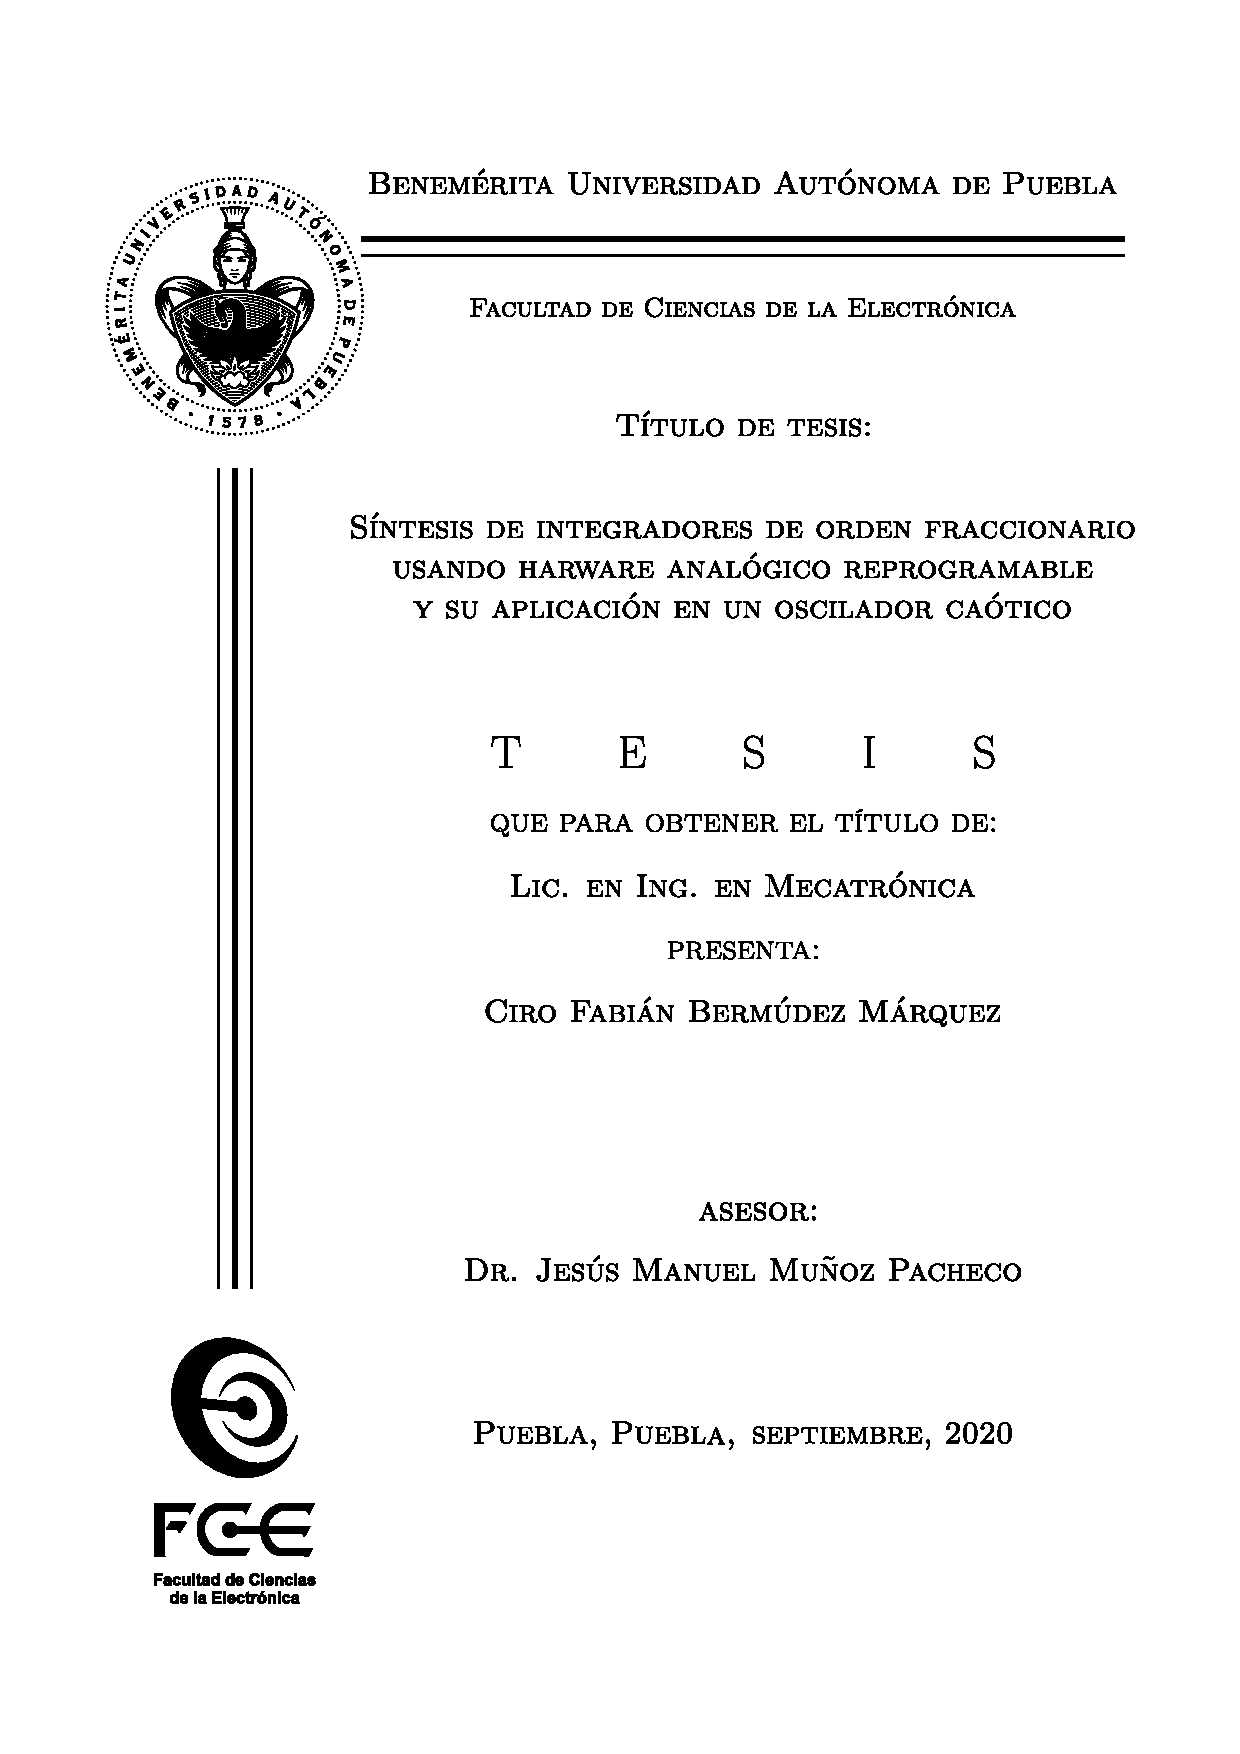
\includepdf[pages=-]{portada2.pdf}
	\thispagestyle{empty}												% Limpiar estilos de pagina

\frontmatter
\onehalfspacing															% Desde este punto interlineado de 1.5
% 	\spacing{1.213}
	\chapter{Agradecimientos}

Agradezco a mi familia ...

Agradezco al CONACYT ...

Agradezco a la Facultad de Ciencias de la Electrónica de la BUAP  ...

\pagestyle{normalstyle}												% Estilos de pagina personalizados
\tableofcontents            											% Genera el índice
\addcontentsline{toc}{chapter}{\contentsname}

\listoffigures              											% Indice de figuras
\listoftables               											% Indice de tablas
\lstlistoflistings

	\chapter{Resumen}


	En este trabajo de tesis se presenta en primera instancia el análisis teórico de la expansión de fracciones continuas (CFE) para su utilización en la creación de integradores de orden fraccionario. Se hace un análisis del error que esta aproximación presenta y se generará una metodología de diseño de acuerdo al orden fraccionario.
	
	Utilizando hardware analógico embebido (FPAA) y por medio del dispositivo NI ELVIS II+ se realizará la implementación física de los integradores de orden fraccionario y se medirá su respuesta en frecuencia. Obtenidos los resultados se obtendrá un análisis comparativo teórico contra experimental y se desarrollaran gráficas de mérito para facilitar el diseño.
	
	Finalmente se utilizarán las metodologias obtenidas para realizar la implementación de un oscilador caótico de orden fraccionario poniendo a prueba así el rendimiento de los integradores.
	\pagestyle{Resumen}	
	
\mainmatter
\pagestyle{normalstyle}	
	\chapter{Introducción}
	
	El caos se refiere a un tipo de comportamiento dinámico complejo que posee algunas características muy especiales, tales como extrema sensibilidad a pequeñas variaciones de la condición inicial, trayectorias encerradas en el espacio de fase pero con un exponente de Lyapunov positivo, un espectro de potencia continuo entre muchas otras. En pocas palabras, el caos es simplemente un comportamiento impredecible de un sistema determinista. Es de interés resaltar que los sistemas caóticos ya eran conocidos desde hace mucho tiempo atrás y que no fue hasta hace poco que se logró demostrar que el caos puede ser controlado y debido a esto impactar en muchas áreas, tanto en áreas cercanas a la electrónica como técnicas de modulación, sistemas de comunicación, técnicas de encriptación de datos, como también en áreas  relacionadas a los sistemas biológicos, reacciones químicas, toma de decisiones críticas en política, economía, eventos militares, etc  \cite{Munoz-Pacheco2010}. El caos es un fenómeno que ocurre en muchos sistemas no lineales, donde la naturaleza determinista de la estructura se conjuga con la irregularidad del comportamiento, esto significa que, a pesar del hecho de que el sistema se describe mediante un conjunto de ecuaciones diferenciales ordinarias, donde todos los términos son perfectamente conocidos, su comportamiento es irregular y muy sensible a las condiciones iniciales. La primera evidencia de imprevisibilidad en los sistemas deterministas se encuentra en el trabajo del matemático y científico Henri Poincaré sobre el movimiento celestial, mientras que la primera formulación del caos en un modelo matemático expresado por un conjunto de ecuaciones diferenciales ordinarias que exhiben el caos se debe al matemático y meteorólogo Edward Lorenz que se encontraba estudiando un modelo de movimiento del aire en la atmósfera y descubrió cómo pequeñas variaciones en los valores iniciales de las variables de su modelo dieron como resultado predicciones meteorológicas divergentes \cite{Buscarino2014}. Para el momento de esos estudios faltaba una prueba experimental definitiva del caos y la tecnología y poder de cómputo no eran suficientes para pensar aún en soluciones y aún más distantes las aplicaciones. Debido al constante avance de la electrónica, hoy en día somos capaces de sintetizar mediante dispositivos electrónicos sistemas caóticos, utilizando técnicas de modelado e implementación es posible crear representaciones de estos, no obstante, todas estas se basan en aproximaciones que aún no han sido exploradas en su totalidad. 
	Por otro lado, el cálculo fraccionario es un tema que tiene más de 300 años de antigüedad y que se remonta a cartas enviadas a Leibniz por parte de Bernoulli y de L'Hôspital preguntando acerca de la derivada a la $1/2$ e indagando sobre su significado. Con el paso de los años la teoría de cálculo fraccionario se fue desarrollando pasando por las manos de nombres conocidos como: Euler, Lagrange, Laplace, Fourier hasta llegar a Liouville, Riemann, Grünwald, Letnikov, Caputo entre muchos otros \cite{Petras2011}. Pero aún con todo ese desarrollo no fue hasta hace poco que la comunidad científica comenzó a interesarse por esta rama del cálculo y la razón principal de este cambio es que los cálculos necesarios para cualquier posible implementación eran demasiado complejos y lentos, un panorama totalmente diferente se vive en la actualidad, el rápido avance de la tecnología ha logrado realizar avances notables en esta área. El rango de aplicaciones para el cálculo fraccionario es inmenso, por mencionar algunas de las más recientes, la modelación de derivadas fraccionarias para obtener una mejor representación comportamental de un sistema industrial metalúrgico \cite{Petras2019}, la incorporación de dinámica de orden fraccionaria para mejorar la robustez de un control PI/PID para motores DC \cite{Tepljakov2016,Khubalkar2018}, la modelación de señales biológicas como ECG, EMG y EEG debido a su respuesta de magnitud de 20$\alpha$dB, modelos fisiológicos basados en ecuaciones diferenciales lineales que describen fenómenos complejos en el cuerpo humano como la oxigenación de la sangre entre otros \cite{Ortigueira2011}.
	El cálculo fraccionario y los sistemas caóticos se complementan al añadir un nivel de profundidad en la creación de osciladores caóticos modelados como un conjunto de ecuaciones diferenciales no lineales fraccionarias las cuales son materia prima para la creación de nuevas aplicaciones y áreas de desarrollo. 
	
	\section{Justificación}
	
	Los osciladores caóticos son una área de oportunidad emergente cuyas aplicaciones han aumentado en los últimos años, a principios del siglo XX se comenzó a explorar el uso de osciladores caóticos para la detección de señales pequeñas basados en la propiedad  de extrema sensibilidad a pequeños cambios de la condición inicial que estos presentan \cite{Wang1999}, y en la seguridad de sistemas de comunicación ya sea en tiempo continuo o discreto \cite{Tepina2002}.  Casi al mismo tiempo los sistemas de orden fraccionario comenzaron nuevamente a formar parte del interés de la comunidad científica  y se abrieron las puertas al control de sistemas de orden fraccionario y cómo implementarlos \cite{Chen2009,Das2007}. Los intentos de implementaciones físicas de sistemas de orden fraccionario han avanzado mucho recientemente y se pueden categorizar en digitales, los cuales utilizan sistemas discretos basados en microprocesadores o FPGAs cuya complejidad radica en poder generar un software robusto que sea lo suficiente confiable \cite{Gunay2017}. Por el otro lado se encuentran las implementaciones analógicas, las cuales son de gran interés en este trabajo. En la literatura de esta área podemos encontrar implementaciones basadas en la construcción de capacitores electrolíticos especiales que se aproximan al comportamiento fraccionario pero cuya fabricación es compleja \cite{Jesus2008}, métodos electro-químicos que trabajan con compuestos de difícil manipulación y tienen ordenes que no pueden modificarse fácilmente \cite{Biswas2006}, finalmente y en lo que se enfocará este trabajo se encuentran las aproximaciones de funciones racionales en un ancho de banda determinado utilizando los métodos de Newton, Oustaloup, Carlson, Matsuda o expansión de fracciones continuas (CFE) \cite{Charef2006,Krishna2011,Krishna2008}. Una vez que la función de trasferencia es obtenida, esta se sintetiza utilizando diferentes metodologías, como la realización pasiva que hace uso de resistencias, capacitores e inductores, con el inconveniente de poder ajustarse a los valores comerciales, o la realización activa, que utiliza las técnicas de diseño basadas en amplificadores operacionales \cite{Tepljakov2013, Dorcak2012}. Una alternativa a estas metodologías es la sintetización utilizando dispositivos analógicos embebidos programables FPAA (Field Programable Analog Array). Las FPAA han demostrado ser una arquitectura prometedora que facilita mucho el proceso de implementación de circuitos analógicos debido a que su interfaz se basa en Módulos Analógicos Configurables (CAM), los cuales son bloques que pueden interconectarse fácilmente y representan desde circuitos sencillos como integradores, derivadores, sumadores o inversores hasta circuitos más complejos como filtros completos y multiplicadores \cite{Fragoulis2009}. Sin embargo en el ámbito tanto de integradores fraccionarios como de osciladores caóticos aún existen metodologías nuevas por explorar, en algunos artículos científicos ya se ha mostrado cómo implementar un integrador de orden fraccionario utilizando la aproximación de Oustaloup y CAMs de filtros bilineales \cite{Caponetto2006}, no obstante la cantidad de recursos para crear un solo integrador es muy grande, lo cual da pie a ser mejorado utilizando aproximaciones diferentes, para este trabajo, la expansión de fracciones continuas. La implementación de osciladores caóticos basados en sistemas de ecuaciones diferenciales de orden entero utilizando una FPAA ya ha sido explorada en años recientes \cite{Li2018}, sin embargo los basados en sistemas de ecuaciones diferenciales de orden fraccionario aun se encuentran en una etapa temprana y son ideales para ser estudiados. Las aplicaciones de los osciladores caóticos van en aumento y ser capaces de implementarlos se ha vuelto una tarea relevante. Sistemas similares a estos en la actualidad se están utilizando en aplicaciones médicas, como en la detección de señales cardíacas \cite{Jiang2010} y en la creación de radares UWB que tienen un futuro prometedor en la medicina \cite{Kumari2017}.
	
	\section{Objetivos}
	
		\subsection{Objetivo general}
			Diseño e implementación electrónica de integradores de orden fraccionario mediante la expansión de fracciones continuas para su aplicación en sistemas caóticos.		
		
		\subsection{Objetivos específicos}
			\begin{itemize}
			\item Analizar el método de expansión de fracciones continuas para generar una metodología de diseño en MATLAB.
			\item Caracterizar el error de la expansión de fracciones continuas para generar reglas de diseño.
			\item Diseñar e implementar en FPAA integradores de orden fraccionario con aproximaciones de ordenes superiores.
			\item Medir la respuesta en frecuencia de los integradores de orden fraccionario y comparar los resultados experimentales y teóricos.
			\item Diseñar e implementar de FPAA un oscilador caótico de orden fraccionario. 
		\end{itemize}
		
		
%% Para formato de propuesta de tesis
\begin{comment}
	\section{Descripción}

	Este trabajo se desarrollará haciendo en primer lugar una investigación profunda del método de expansión de fracciones continuas para la creación de integradores de orden fraccionario y un análisis de su estructura matemática para generar algoritmos eficientes que obtengan la función racional aproximada. Una vez obtenidos estos algoritmos se hará un análisis del error de la función racional aproximada con respecto al integrador fraccionario ideal dependiente del orden de la aproximación y el orden fraccionario. Una vez concluidos los análisis teóricos se procederá a realizar la implementación física de los integradores fraccionarios utilizando la tarjeta Quad Apex v2.0 la cual contiene 4 FPAA. Se realizará un análisis de las diferentes metodologías que se pueden seguir en la implementación haciendo mediciones de la respuesta en frecuencia (Diagramas de Bode). Se pretende que estas mediciones den como resultado reglas de diseño que faciliten el proceso de implementación y mejoren en manejo de recursos en la FPAA. Finalmente se implementará físicamente un oscilador caótico basado en un sistema de ecuaciones diferenciales de orden fraccionario.
	
	\newpage
	\section{Diagrama de bloques}	
	\begin{figure}[hbtp]
	\centering
	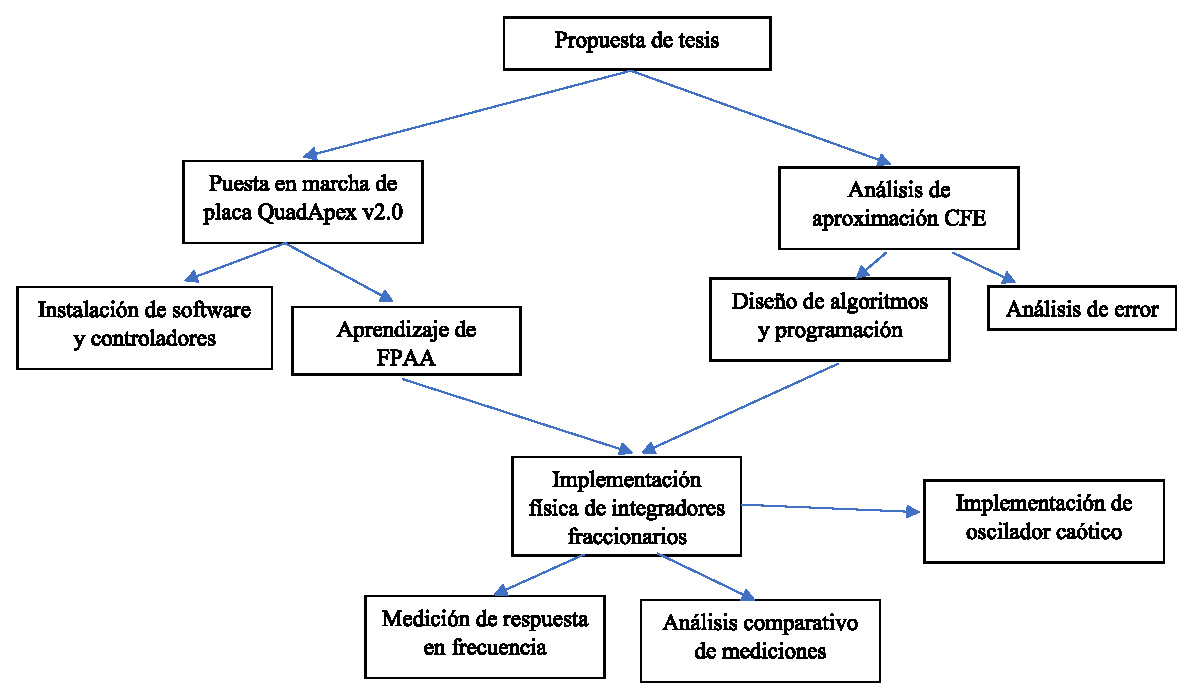
\includegraphics[width = 11cm]{diagrama_de_bloques.eps}
	\caption{Diagrama de bloques}
	\end{figure}
	
	\section{Cronograma de actividades}
	\begin{figure}[hbtp]
	\centering
	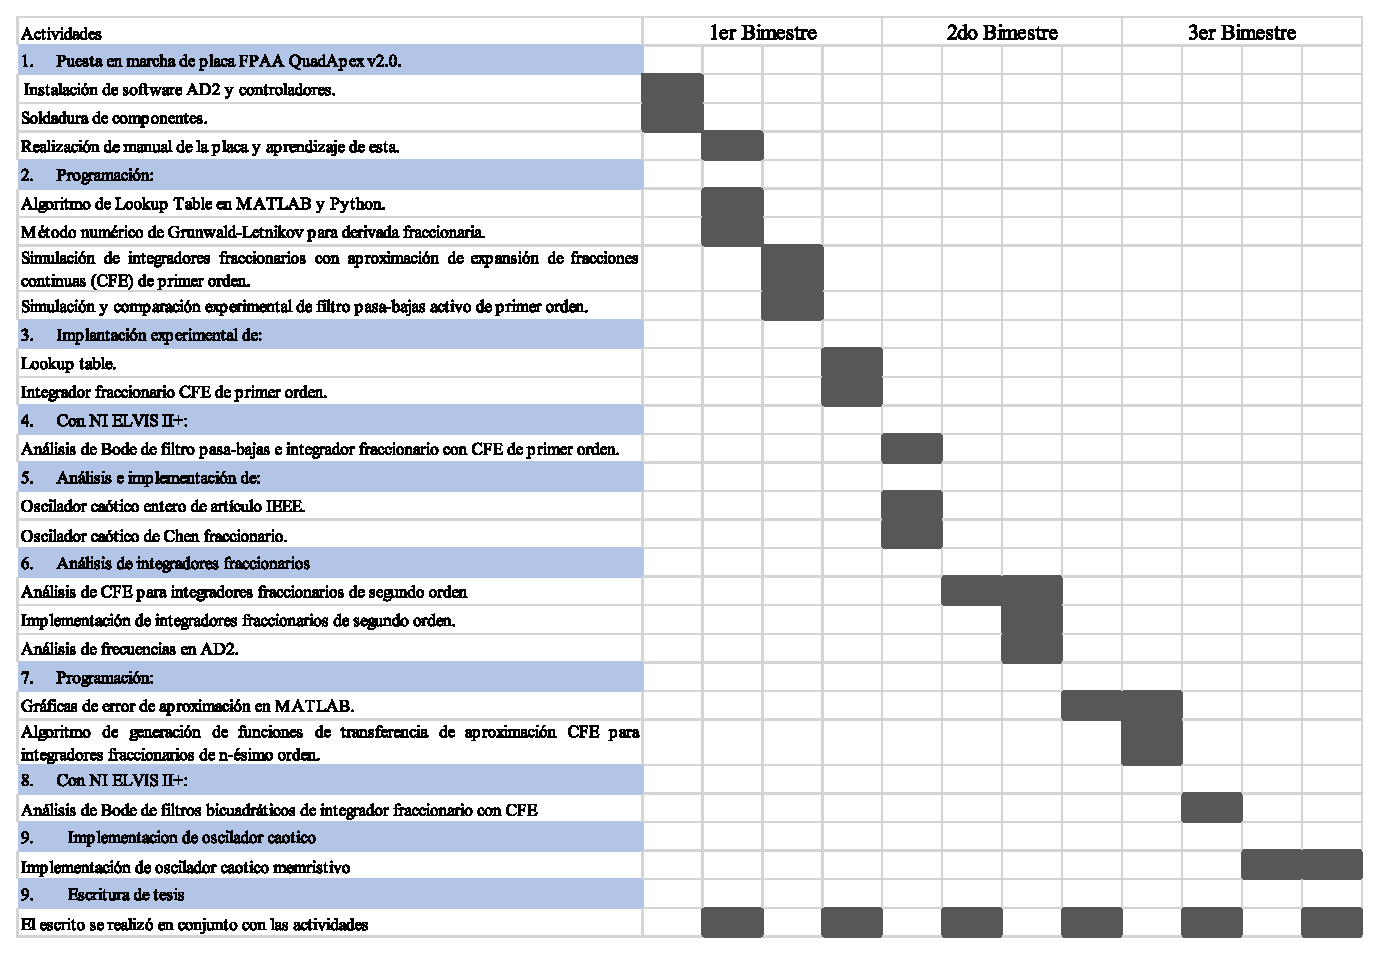
\includegraphics[width = 14.8cm]{cronograma_de_actividades.eps}
	\caption{Cronograma de actividades}
	\end{figure}		
		
\end{comment}
		
	
	
	
	
	\chapter{Fundamentos teóricos}		

	Al igual que cuando se comienza a estudiar cálculo de orden entero, es necesario familiarizarse con la notación de los operadores matemáticos de la derivada y la integral. En la actualidad la notación más utilizada para el cálculo entero es la dada por Leibniz en (1686), donde el operador diferencial de n-ésimo orden esta definido como: $\frac{d^{n}}{dt^{n}}$, $D_{t}^{n}$ o simplemente $D^{n}$ con $n \in \mathbb{N}$. Utilizando el mismo razonamiento, puede definirse su operador inverso (antiderivada) de manera que el operador inverso de la derivada de n-ésimo orden está dado por: $_{a}D^{-n}_{t}$, donde $n \in \mathbb{N}$ y $a \in \mathbb{R}$ representa el límite inferior del dominio de la región donde se aplica dicho operador.
			
	Para generalizar el operador diferencial e integral para orden fraccionario se considera que este puede definirse para parámetros de orden real o incluso complejo. Esto implica que los operadores pueden definirse respectivamente como: $D^{\alpha}$ y $_{a}D^{\alpha}_{t}$ con $ \alpha \in \mathbb{R}$. 
		
	Es importante resaltar que no una hay una única definición de operadores diferencial fraccional ni integral sino varias expresiones definidas por diferentes autores, entre las mas usadas se encuentran la definición de Grünwald-Letnikov (GL), la de Riemann-Liouville (RL) y la de Caputo (Ca), cada una de estas con sus ventajas y desventajas desde el punto de vista del análisis matemático, complejidad computacional e implementación \cite{Petras2011}.
			
	\section{Definición de Grünwald-Letnikov}

	Comenzamos considerando que para el caso de orden entero la n-ésima derivada para una función $f$ con $n \in \mathbb{N}$ y $j>n$ esta dada por:
	\begin{equation}
		f^{(n)}(t) = \frac{d^{n}f}{dt^{n}} = \lim_{h \to 0 } \frac{1}{h^{n}} \sum_{j = 0}^{n} (-1)^{j} \binom{n}{j} f(t - jh)
		\label{ec:derivada_entera}
	\end{equation}
	donde $\binom{n}{j}$ representa el coeficiente binomial dado por la expresión:
			
	\begin{equation}
		\binom{n}{j} = \frac{n!}{j! (n-j)! } 
	\end{equation}
			
	Considerando valores negativos de $n$ tenemos:
	\begin{equation}
		\binom{-n}{j} = \frac{-n(-n-1)(-n-2) \cdots (-n -j +1 )}{j!}= (-1)^{j} \binomb{n}{j}
		\label{ec:binomio_n}
	\end{equation}
	donde $\binomb{n}{j}$ esta definido como:
			
	\begin{equation}
		\binomb{n}{j} = \frac{2(n+1) \cdots (n+j-1)}{j!}
	\end{equation}
	
		\subsection{Definición de derivada de Grünwald-Letnikov}
		
	Generalizando la ecuación (\ref{ec:derivada_entera}) podemos escribir la definición de derivada de orden fraccionario de orden  $\alpha$, ($\alpha \in \mathbb{R}$) como:
		
	\begin{equation}
		D^{\alpha}_{t} f(t) = \lim_{h \to 0} \frac{1}{h^{\alpha}}   \sum_{j = 0}^{\infty} (-1)^{j} \binom{\alpha}{j} f(t - jh)
		\label{ec:derivada_frac_GL}
	\end{equation}
			
	Para calcular el coeficiente binomial podemos utilizar la relación entre la función Gamma de Euler y el factorial definido como:
	\begin{equation}
		\binom{\alpha}{j}  = \frac{\alpha!}{j! (\alpha-j)!} = \frac{\Gamma (\alpha + 1)}{\Gamma(j+1) \Gamma(\alpha - j + 1)}
	\end{equation}
	donde la función Gamma de Euler con $r>0$ esta definida como:
			
	\begin{equation}
		\Gamma(r) = \int^{\infty}_{0} t^{r-1} e^{-t}dt
	\end{equation}
			
		\subsection{Definición de integral de Grünwald-Letnikov}
		
	Utilizando la ecuación (\ref{ec:derivada_frac_GL}) se puede definir un operador de tipo integral para la función $f$  sobre el dominio temporal $(a,t)$ considerando $n = \frac{t-a}{h}$ donde $a \in \mathbb{R}$ como:
			
	\begin{equation}
		_{a}D_{f}^{\alpha} = \lim_{h \to 0 } \frac{1}{h^{\alpha}} \sum_{j = 0}^{\left[ \frac{t-a}{h}  \right]} (-1)^{j} \binom{n}{j} f(t - jh)
	\end{equation}

		\subsection{Método numérico para la definición de GL}
		
	Utilizando como base la ecuación (\ref{ec:derivada_frac_GL}) esta se puede discretizar para los puntos $kh$, ($k = 1,2,\ldots$) de la siguiente manera:
			
	\begin{equation}
		_{\left( \frac{L_{m}}{h} \right)} D^{\alpha}_{t_{k}} f(t) \approx \frac{1}{h^{\alpha}} \sum_{j=0}^{k}(-1)^{j}  \binom{\alpha}{j} f(t_{k-j})
	\end{equation}
	donde $L_{m}$ es el tamaño de memoria (memory length), $t_{k} = kh$, $h$ es el paso de tiempo del cálculo y $(-1)^{j}\binom{\alpha}{j}$ son coeficientes binomiales $C_{j}^{(\alpha)}$ $(j=0,1,\ldots)$. Para su calculo utilizamos la siguiente expresión:
		
	\begin{equation}
		C_{0}^{(\alpha)} = 1, \qquad  C_{j}^{(\alpha)} = \left( 1 - \frac{1 + \alpha}{j} \right) C_{j-1}^{(\alpha)}
	\end{equation}
			
	Entonces, la solución numérica general de la ecuación diferencial fraccional:
		
	\begin{equation}
	 	_{a}D^{\alpha}_{t} y(t) = f(y(t), t)
	\end{equation}
	puede expresarse como:
		
	\begin{equation}
		y(t_{k}) = f(y(t_{k-1}), t_{k-1}) h^{\alpha} - \sum_{j=1}^{k} C_{j}^{(\alpha)} y(t_{k-j})
		\label{ec:GL_numerico}
	\end{equation}

	Para el termino de la memoria expresada por la sumatoria, el principio de memoria corta puede utilizarse. Entonces el indice superior de la sumatoria en la ecuación (\ref{ec:GL_numerico}) se cambiará por $\nu$ con las siguientes consideraciones: se usa $\nu = k$ para $k < \left( \frac{L_{m}}{h} \right)$ y $\nu = \left( \frac{L_{m}}{h} \right)$ para $k \geq (\frac{L_{m}}{h})$, o sin usar el principio de memoria corta se utiliza $\nu = k$ para toda $k$. 
	
	\section{Definición de Riemann-Liouville}
	
	Para esta definición consideramos la fórmula de Cauchy para la integral repetida que esta dada por:
	
	\begin{equation}
		f^{(-n)} (t) = \int_{a}^{t} \int_{a}^{\sigma_{1}}  \cdots \int_{a}^{\sigma_{n-1}} f(\sigma_{n}) d\sigma_{n} \cdots d\sigma_{2} d\sigma_{1} = \frac{1}{(n - 1)!} \int^{t}_{a} \frac{f(\tau)}{(t - \tau)^{1 - n}} d \tau
		\label{ec:cauchy}
	\end{equation}

		\subsection{Definición de integral de Riemann-Liouville}
		
	Utilizando las propiedades de la función Gamma de Euler con el factorial y la ecuación (\ref{ec:cauchy}) se puede escribir la definición de integral fraccionaria como:

	\begin{equation}
		_{a}D_{t}^{-\alpha} f(t) = \frac{1}{\Gamma( \alpha)} \int_{a}^{t} \frac{f(\tau)}{(t - \tau)^{ 1 - \alpha}} d \tau
		\label{ec:integral_RL}
	\end{equation}
	para $\alpha<0$ y $a \in \mathbb{R}$. No obstante para el caso de $0 < \alpha < 1$ y $f(t)$ siendo una función casual, esto es, $f(t)=0$ para $t<0$, la integral fraccionaria esta definida como:
	
	\begin{equation}
		_{0}D_{t}^{-\alpha} f(t) = \frac{1}{\Gamma( \alpha)} \int_{0}^{t} \frac{f(\tau)}{(t - \tau)^{ 1 - \alpha}} d \tau , \quad \mathrm{para} \quad 0 < \alpha < 1, \quad t > 0
	\end{equation}
		
		\subsection{Definición de derivada de Riemann-Liouville}
		
	De la ecuación (\ref{ec:integral_RL}) se puede escribir la definición de derivada fraccionaria de orden $\alpha$ de la siguiente manera:
	
	\begin{equation}
		_{a}D_{t}^{\alpha} f(t) = \frac{1}{\Gamma(n - \alpha)} \frac{d^{n}}{dt^{n}} \int_{a}^{t} \frac{f(\tau)}{(t - \tau)^{\alpha - n + 1}} d \tau
	\end{equation}
	donde $(n-1 < \alpha < n)$. Pero igual que con la integral si consideramos $0 < \alpha < 1$ y $f(t)$  una función casual, la derivada de orden fraccionaria se puede reescribir como:
	
	\begin{equation}
		_{0}D_{t}^{\alpha}f(t) = \frac{1}{\Gamma(n-\alpha)} \frac{d^{n}}{dt^{n}} \int_{0}^{t} \frac{f(\tau)}{(t - \tau)^{\alpha - n + 1}} d\tau
	\end{equation}
		
	\section{Transformada de Laplace de integrales y derivadas fraccionarias}
	
	La transformada de Laplace de la integral fraccionaria ya sea para Riemman-Liouville o para Grünwald-Letnikov esta definida como:
	
	\begin{equation}
	 	\mathcal{L} \{ _{0}D_{t}^{-p} f(t) \} = s^{-p} F(s)
	\end{equation} 
	y dadas condiciones iniciales cero  la transformada de Laplace de la derivada fraccionaria de orden $r$ para Grünwald-Letnikov, Riemann-Liouville y Caputo se reduce a:
	
	\begin{equation}
		\mathcal{L} \{ _{0}D_{t}^{r} f(t) \} = s^{r} F(s)
	\end{equation}
	
	
	\section{Expansión de fracciones continuas (CFE)}
	
	A una expresión de la forma:

	\begin{equation}
		a_{1} + \cfrac{b_{1}}{a_{2} + \cfrac{b_{2}}{a_{3} + \cfrac{b_{3}}{a_{4} + \genfrac{}{}{0pt}{0}{}{\ddots}}}}
		\label{ec:fracciones_cont}
	\end{equation} 
	se le conoce como una fracción continua. En general $a_{1},a_{2},a_{3}, \cdots, b_{1}, b_{2}, b_{3}$ pueden ser cualquier número real o complejo, y el número de términos pueden ser finito o infinito.

	Una manera más conveniente de escribir la ecuación (\ref{ec:fracciones_cont}) es:

	\begin{equation}
		a_{1} + \frac{b_{1}}{a_{2} } \genfrac{}{}{0pt}{0}{}{+}   \frac{b_{2}}{a_{3}}  \genfrac{}{}{0pt}{0}{}{+}  \frac{b_{3}}{a_{4}}  \genfrac{}{}{0pt}{0}{}{+}  \genfrac{}{}{0pt}{0}{}{\cdots} 
		\label{ec:fracciones_cont_sim}
	\end{equation}
	y es la que se encontrará normalmente en libros y artículos. Ambas notaciones son  muy similar y se puede pasar de una a otra sin mayor complicación.

	De la ecuación (\ref{ec:fracciones_cont_sim}) se pueden formar las siguientes fracciones:

	\begin{equation}
		c_{1} = \frac{a_{1}}{1} , \quad c_{2} = a_{1} + \frac{b_{1}}{a_{2}}, \quad c_{3} = a_{1} + \frac{b_{1}}{a_{2}} \genfrac{}{}{0pt}{0}{}{+} \frac{b_{2}}{a_{3}}, \quad \cdots
	\end{equation}
	las cuales se obtienen, en sucesión, de cortar el proceso de expansión después del primer, segundo, tercer, $\cdots$ término. Estas fracciones son llamadas primer, segundo, tercer, $\cdots$  convergente, respectivamente, de la fracción continua. El $n$-ésimo convergente es:

	\begin{equation}
		c_{n} = a_{1} + \frac{b_{1}}{a_{2}} \genfrac{}{}{0pt}{0}{}{+} \frac{b_{2}}{a_{3}} \genfrac{}{}{0pt}{0}{}{+} \genfrac{}{}{0pt}{0}{}{\cdots} \genfrac{}{}{0pt}{0}{}{+} \frac{b_{n-1}}{a_{n}}
	\end{equation}

	En 1776 Lagrange obtuvo la expansión de fracciones continuas (CFE) para la ecuación $(1 + x)^{\alpha}$ como se muestra a continuación \cite{Olds2009}:

	\begin{equation}
 		(1 + x)^{\alpha} = \cfrac{1}{1 - \cfrac{\alpha x}{1 + \cfrac{\cfrac{1(1 + \alpha)}{1\cdot2}\,x}{1 + \cfrac{\cfrac{1(1 - \alpha)}{2\cdot3}\,x}{1 + \cfrac{\cfrac{2(2 + \alpha)}{3\cdot4}\,x}{1 + \cfrac{\cfrac{2(2 - k)}{4\cdot5}\,x}{1 + \cfrac{\cfrac{3(3 + \alpha)}{5\cdot6}\,x}{1 + \genfrac{}{}{0pt}{0}{}{\ddots}}}}}}}}
		 \label{ec:lagrange}
	\end{equation}
	y escrita de una manera más compacta:

	\begin{equation}
 		(1 + x)^{\alpha} = \frac{1}{1} \genfrac{}{}{0pt}{0}{}{-} \frac{\alpha x}{1} \genfrac{}{}{0pt}{0}{}{+} \frac{\frac{1(1 + \alpha)}{1\cdot2}\,x}{1} \genfrac{}{}{0pt}{0}{}{+} \frac{\frac{1(1 - \alpha)}{2\cdot3}\,x}{1} \genfrac{}{}{0pt}{0}{}{+} \frac{\frac{2(2 + \alpha)}{3\cdot4}\,x}{1} \genfrac{}{}{0pt}{0}{}{+} \frac{\frac{2(2 - \alpha)}{4\cdot5}\,x}{1} \genfrac{}{}{0pt}{0}{}{+} \genfrac{}{}{0pt}{0}{}{\cdots} 
		\label{ec:lagrange_conv}
	\end{equation}
	la ecuación (\ref{ec:lagrange_conv}) puede reescribirse convenientemente multiplicando un $m$ en el numerador y en el denominador como se muestra a continuación:

	\begin{equation}
 		(1 + x)^{\alpha} = \frac{1}{1} \genfrac{}{}{0pt}{0}{}{-} \frac{\alpha x}{1} \genfrac{}{}{0pt}{0}{}{+}  \frac{ {\color{red} 2} \cdot \frac{1(1 + \alpha)}{1\cdot2}\,x}{{\color{red} 2} \cdot 1} \genfrac{}{}{0pt}{0}{}{+} \frac{ {\color{blue} 3} \cdot {\color{red} 2} \cdot \frac{1(1 - \alpha)}{2\cdot3}\,x}{{\color{blue} 3} \cdot 1} \genfrac{}{}{0pt}{0}{}{+} \frac{{\color{blue} 3} \cdot \frac{2(2 + \alpha)}{3\cdot4}\,x}{1}   \genfrac{}{}{0pt}{0}{}{+} \genfrac{}{}{0pt}{0}{}{\cdots} 
	\end{equation}
	hay que notar que cada denominador esta compuesto por 2 términos, esto se puede ver claramente en la ecuación (\ref{ec:lagrange}), y que contando el término del numerador, $m$ se tiene que agregar en 3 lugares distintos. Si se eligen $m_{1} = 2$, $m_{2} = 3$, $m_{3} = 2$, $\ldots$ de manera que se simplifique la ecuación obtenemos:

	\begin{equation}
 		(1 + x)^{\alpha} = \frac{1}{1}  \genfrac{}{}{0pt}{0}{}{-} \frac{\alpha x}{1} \genfrac{}{}{0pt}{0}{}{+} \frac{(1 + \alpha)x}{2} \genfrac{}{}{0pt}{0}{}{+} \frac{(1 - \alpha)x}{3} \genfrac{}{}{0pt}{0}{}{+} \frac{(2 + \alpha)x}{2} \genfrac{}{}{0pt}{0}{}{+} \frac{(2-\alpha)x}{5} \genfrac{}{}{0pt}{0}{}{+} \genfrac{}{}{0pt}{0}{}{\cdots}
 		\label{ec:cfe_inutil}
	\end{equation}

	La ecuación (\ref{ec:cfe_inutil}) se puede encontrar en distintos artículos \cite{Krishna2008,Krishna2011}, no obstante para programar un algoritmo que obtenga la aproximación de $(1 + x)^{\alpha}$ hasta el $n$-ésimo convergente resulta poco intuitiva. Para este fin la ecuación (\ref{ec:lagrange_conv}) resulta más sencilla y contiene un patrón que puede explotarse.

	El $n$-ésimo término de la expansión de fracciones continuas para la ecuación (\ref{ec:lagrange_conv}) se puede calcular utilizando la siguiente ecuación:

	\begin{equation}
		\frac{\psi(n) \left[ \psi(n) + (-1)^{n} \alpha \right]}{(n-1)n}
		\label{ec:calculo_terminos_cfe}
	\end{equation}
	donde la función $\psi(x)$ para $x\geq2$, $x\in \mathbb{Z}^{+}$ esta definida como\footnote{$\left\lfloor x\right\rfloor$ es  la función redondeo hacia el entero inferior anterior.}:

	\begin{equation}
		\psi(x) = \left\lfloor \frac{x}{2}\right\rfloor
	\end{equation}

	La ecuación (\ref{ec:calculo_terminos_cfe}) se puede utilizar de manera recursiva desde el $n$-ésimo término hasta el segundo sin olvidar que cada uno de estos siempre debe ir acompañado de la suma de un uno. También vale la pena resaltar que el primer término de la expansión es $\cfrac{1}{1} \genfrac{}{}{0pt}{0}{}{-} \cfrac{\alpha x}{1}$ en conjunto. 

	Sustituyendo $x = s - 1$ y limitando el número de términos de la ecuación (\ref{ec:lagrange_conv}) obtenemos la aproximación racional para $s^{\alpha}$ y para obtener la aproximación racional de $\frac{1}{s^{\alpha}}$ la expresión tiene que ser simplemente invertida. En el apéndice \ref{cod:cfetf} se muestra un programa en MATLAB que calcula la aproximación para un integrador fraccionario de orden $\alpha$ eligiendo el número de términos $n$, utilizando el método de CFE descrito previamente.

	En general la aproximación utilizando la CFE para un integrador fraccionario $\frac{1}{s^{\alpha}}$ utilizando los primeros dos términos resulta en una función de transferencia de primer orden como se muestra a continuación:

	\begin{equation}
		\genfrac{}{}{0pt}{0}{}{_{(c_{2})}} \frac{1}{s^{\alpha}} \approx \frac{(1 - \alpha)s + (1 + \alpha) }{(1 + \alpha)s + (1 - \alpha)} 
	\end{equation}

	Al utilizar un número impar de términos el grado del numerador de la función de transferencia siempre será mayor en uno al del denominador, además de que el coeficiente de mayor grado del numerador siempre tendrá signo negativo, esto resulta problemático en la implementación y debido a estas observaciones es recomendable solo trabajar con un número par de términos.

	La aproximación de segundo orden tiene la forma:

	\begin{equation}
		\genfrac{}{}{0pt}{0}{}{_{(c_{4})}} \frac{1}{s^{\alpha}} \approx \frac{(\alpha^{2} - 3\alpha + 2) s^{2} + (8 - 2 \alpha^{2})s + (\alpha^{2} + 3\alpha + 2) }{(\alpha^{2} + 3\alpha + 2) s^{2} + (8 - 2 \alpha^{2})s + (\alpha^{2} - 3\alpha + 2)}
	\end{equation}
la ventaja de utilizar la aproximación de CFE es que convertimos el problema de orden fraccionario a uno de orden entero de manera sistemática. Por ejemplo para un integrador de orden fraccionario con $\alpha = 0.5$ sus aproximaciones son las mostradas en la Tabla \ref{tab:aprox_cfe_alpha_0.5} y sus correspondientes diagramas de bode se muestran en la Figura \ref{fig:F1_bode_integrador_alpha05}.


	\begin{table}[!hbp]
		\caption{Aproximaciones racionales de $\frac{1}{s^{0.5}}$}
		\label{tab:aprox_cfe_alpha_0.5}
		\centering
%		\resizebox{\textwidth}{!}{
		\begin{tabular}{c c c}
			\hline
			\textbf{Orden} &  \textbf{No. de términos} & \textbf{Aproximación racional}\\
			\hline
			$1$ 		& $2$ 		&  $\cfrac{s + 3}{3s + 1}$\\
					 		& 		 		& \\
			$2$			& $4$ 		&  $\cfrac{s^{2} + 10s + 5}{5 s^{2} + 10s + 1}$\\
							& 		 		& \\
			$3$ 		& $6$ 		&  $\cfrac{s^{3} + 21s^{2} + 35s + 7}{7 s^3 + 35 s^2 + 21 s + 1}$	\\
							& 		 		& \\
			$4$ 		& $8$ 		&  $\cfrac{s^4 + 36 s^3 + 126 s^2 + 84 s + 9}{9 s^4 + 84 s^3 + 126 s^2 + 36 s + 1}$\\
							& 		 		& \\
			$5$ 		& $10$ 		&  $\cfrac{s^5 + 55 s^4 + 330 s^3 + 462 s^2 + 165 s + 11}{11 s^5 + 165 s^4 + 462 s^3 + 330 s^2 + 55 s + 1}$\\
							& 		 		& \\
			\hline
		\end{tabular}
%		}
	\end{table}
	
	Analizando la Figura \ref{fig:F1_bode_integrador_alpha05} se puede resaltar que en general la aproximación aumenta su ancho de banda conforme el orden de la función de transferencia aumenta y que de mismo modo el error con respecto al integrador ideal disminuye, lo cual era de esperarse, el ancho de banda útil es de $10^{-1}$ rad/s hasta $10^{1}$ rad/s, es decir aproximadamente dos décadas, no obstante un análisis más profundo es necesario para notar otras peculiaridades que ocurren en este tipo de aproximaciones.
	
	\begin{figure}[hbtp]
	\caption{Diagramas de bode comparativos de integrador fraccionario, funciones de transferencia de primer hasta quito orden.} 
	\label{fig:F1_bode_integrador_alpha05}
	\centering
	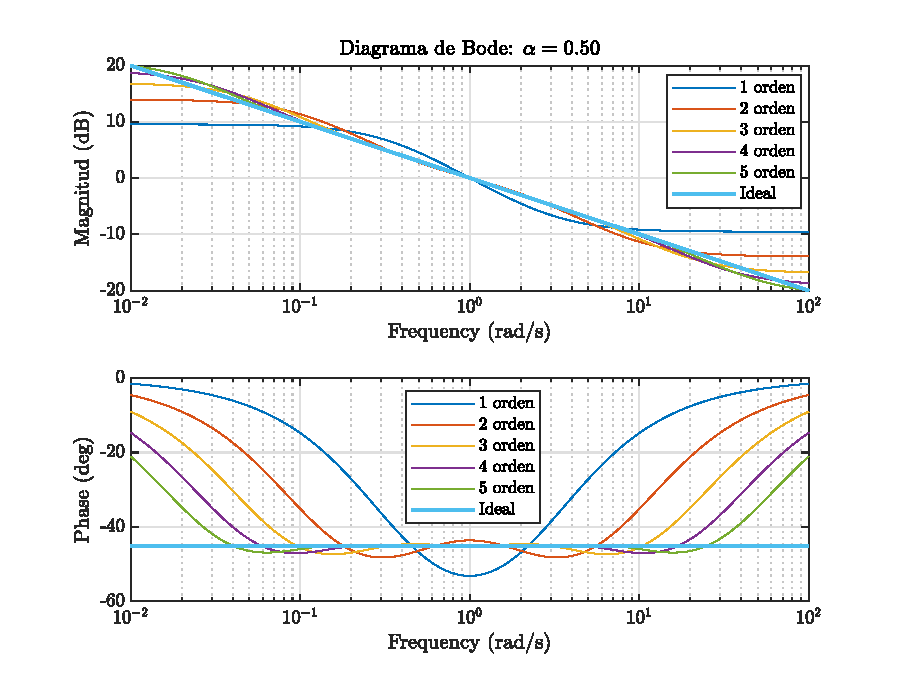
\includegraphics[width=12cm]{F1_bode_integrador_alpha05.eps}
	\end{figure}
	
	\subsection{Análisis de error de la CFE}
	Si variamos el orden $\alpha$ del integrador y el orden de la función de transferencia aproximada podemos notar que entre más pequeño sea $\alpha$ más se alejada la aproximación con respecto a un integrador fraccionario ideal, esto considerando el ancho de banda útil (ver Figuras \ref{fig:analisis_mag}, \ref{fig:analisis_fase}). Para cuantificar lo anterior existen dos tipos de errores de interés, el error sin normalizar y el error normalizado.
	
	El error en dB de la magnitud sin normalizar se puede calcular utilizando la siguiente ecuación:
	\begin{equation}
	\mathrm{error}_{\mathrm{dB}} = 20\log_{10} \left| \frac{H(j\omega)}{G(j\omega)} \right|
	\label{ec:error_sin_norm}
	\end{equation}
	donde $H(j\omega)$ es el integrador ideal $\frac{1}{s^{\alpha}}$ y $G(j\omega)$ es la función de transferencia aproximada del integrador utilizando CFE $ _{(c_{n})} \frac{1}{s^{\alpha}}$. 
	
	El error en grados de la fase sin normalizar se obtiene utilizando la siguiente ecuación:
	
	\begin{equation}
	\mathrm{error}_{\mathrm{deg}} = \phase{H(j\omega)} - \phase{G(j\omega)}
	\end{equation}
	
	Debido a que un integrador fraccionario ideal es en esencia un polo en el origen elevado a una potencia, este tiene un comportamiento de $-20 \alpha$ dB/década en magnitud y de $-90\alpha$ grados en fase \cite{CharlesAlexander2016}, para normalizar el error este hecho resulta importante ya que la magnitud del integrador ideal en $0.1$ rad/seg para cualquier $\alpha$ siempre será $20 \alpha$ dB y para $10$ rad/seg de $-20 \alpha$ dB, de manera similar la fase permanece constante en $-90\alpha$ grados para cualquier $\alpha$.
	
	Entonces la ecuación para el error normalizado de magnitud es:
	
	\begin{equation}
	\mathrm{error}_{\mathrm{norm\,\,de\,\,mag}} = \cfrac{ 20\log_{10} \left| \frac{H(j\omega)}{G(j\omega)} \right| }{20 \alpha} = \cfrac{ \log_{10} \left| \frac{H(j\omega)}{G(j\omega)} \right| }{ \alpha}
	\end{equation}
	y la ecuación para el error normalizado de fase es:
	
	\begin{equation}
	\mathrm{error}_{\mathrm{norm\,\,de\,\,fase}} = \cfrac{\phase{H(j\omega)} - \phase{G(j\omega)}}{90\alpha}
	\end{equation}
	
	Para poder comparar los errores de manera precisa se debe calcular el valor absoluto de los errores para tener una medida de cuanto se aleja del integrador fraccionario ideal. En las Tablas \ref{tab:max_error_mag} y \ref{tab:max_error_fase} se muestran los errores absolutos máximos sin normalizar para la magnitud y la fase dependiente de $\alpha$ y el orden de la función de transferencia, estos datos se puede corroborar dirigiéndose a las gráficas de las Figuras \ref{fig:analisis_error_mag} y \ref{fig:analisis_error_fase}.
	
\begin{table}[!hbp]                                 
\centering            
\caption{Máximo error absoluto de magnitud en dB variando $\alpha$ y orden de función de transferencia.}                           
\label{tab:max_error_mag}                               
\begin{tabular}{cccccc}
\hline                                             
$\,\,\,\,\bm{\alpha}$\textbf{/Orden} & \textbf{1$^{\mathrm{er}}$} & \textbf{2$^{\mathrm{do}}$} & \textbf{3$^{\mathrm{er}}$} & \textbf{4$^{\mathrm{to}}$} & \textbf{5$^{\mathrm{to}}$} \\                     
\hline                                             
0.1 & 0.4587 & 0.3333 & 0.2427 & 0.0620 & 0.0220 \\
                                           
0.2 & 0.8931 & 0.6524 & 0.4665 & 0.1172 & 0.0423 \\
                                            
0.3 & 1.2792 & 0.9426 & 0.6527 & 0.1596 & 0.0591 \\
                                            
0.4 & 1.5942 & 1.1889 & 0.7838 & 0.1848 & 0.0710 \\
                                            
0.5 & 1.8155 & 1.3748 & 0.8449 & 0.1904 & 0.0767 \\
                                           
0.6 & 1.9193 & 1.4807 & 0.8259 & 0.1767 & 0.0755 \\
                                            
0.7 & 1.8769 & 1.4676 & 0.7232 & 0.1458 & 0.0669 \\
                                            
0.8 & 1.6464 & 1.2410 & 0.5415 & 0.1021 & 0.0510 \\
                                           
0.9 & 1.1460 & 0.7507 & 0.2939 & 0.0513 & 0.0284 \\
\hline                                             
\end{tabular}                                                             
\end{table}


\begin{table}[!hbp]                                 
\centering            
\caption{Máximo error absoluto de fase en grados variando $\alpha$ y orden de función de transferencia.}                           
\label{tab:max_error_fase}                               
\begin{tabular}{cccccc}
\hline                                             
$\,\,\,\,\bm{\alpha}$\textbf{/Orden} & \textbf{1$^{\mathrm{er}}$} & \textbf{2$^{\mathrm{do}}$} & \textbf{3$^{\mathrm{er}}$} & \textbf{4$^{\mathrm{to}}$} & \textbf{5$^{\mathrm{to}}$} \\                     
\hline                                             
0.1 & 6.7092 & 2.8727 & 0.6548 & 0.5632 & 0.2796 \\ 
                                             
0.2 & 13.2833 & 5.5250 & 1.2598 & 1.0838 & 0.5338 \\
                                            
0.3 & 19.5614 & 7.7297 & 1.7677 & 1.5208 & 0.7390 \\
                                              
0.4 & 25.3200 & 9.2514 & 2.1362 & 1.8358 & 0.8760 \\
                                            
0.5 & 30.2099 & 9.8632 & 2.3294 & 1.9960 & 0.9311 \\
                                             
0.6 & 33.6307 & 9.3936 & 2.3198 & 1.9760 & 0.8975 \\
                                             
0.7 & 34.4722 & 7.8155 & 2.0880 & 1.7611 & 0.7756 \\
                                             
0.8 & 30.6494 & 5.3543 & 1.6237 & 1.3492 & 0.5739 \\
                                             
0.9 & 19.0601 & 2.5243 & 0.9255 & 0.7528 & 0.3080 \\
\hline                                             
\end{tabular}                                                             
\end{table}

	A simple vista se podría creer que el error máximo aumenta conforme aumenta $\alpha$, no obstante esto es falso debido a que no se esta teniendo en cuenta la escala de la gráfica y por lo tanto las Tablas \ref{tab:max_error_mag} y \ref{tab:max_error_fase} únicamente nos dan información del total de error y no del porcentaje. Para tomar en cuenta la escala es necesario normalizar el error y de mismo modo calcular el valor absoluto de este. Las gráficas de la respuesta de magnitud y fase normalizadas se pueden encontrar en las Figuras \ref{fig:analisis_mag_norm} y \ref{fig:analisis_fase_norm}, y las gráficas de los errores normalizados en las Figuras \ref{fig:analisis_error_mag_norm} y \ref{fig:analisis_error_fase_norm}.
	
	En las Tablas \ref{tab:max_error_mag_norm} y \ref{tab:max_error_fase_norm} se muestran los porcentajes del máximo error absoluto normalizados para la magnitud y la fase, haciendo un análisis de estas se puede llegar a la conclusión de que en efecto \textbf{el porcentaje de error es mayor cuanto más pequeño sea $\bm{\alpha}$} y esto es de gran interés para poder generar reglas de diseño para la implementación de circuitos integradores fraccionarios.

\begin{table}[!hbp]                                 
\centering            
\caption{Máximo error absoluto de magnitud normalizado en \% variando $\alpha$ y orden de función de transferencia.}                           
\label{tab:max_error_mag_norm}                               
\begin{tabular}{cccccc}
\hline                                             
$\,\,\,\,\bm{\alpha}$\textbf{/Orden} & \textbf{1$^{\mathrm{er}}$} & \textbf{2$^{\mathrm{do}}$} & \textbf{3$^{\mathrm{er}}$} & \textbf{4$^{\mathrm{to}}$} & \textbf{5$^{\mathrm{to}}$} \\                     
\hline                                             
0.1 & 22.9364 & 16.6661 & 12.1365 & 3.1006 & 1.1022 \\
                                               
0.2 & 22.3267 & 16.3092 & 11.6624 & 2.9299 & 1.0576 \\
                                                
0.3 & 21.3204 & 15.7107 & 10.8780 & 2.6595 & 0.9850 \\
                                               
0.4 & 19.9281 & 14.8618 & 9.7974 & 2.3094 & 0.8869 \\ 
                                               
0.5 & 18.1555 & 13.7481 & 8.4493 & 1.9044 & 0.7669 \\ 
                                                
0.6 & 15.9941 & 12.3390 & 6.8823 & 1.4724 & 0.6290 \\ 
                                              
0.7 & 13.4063 & 10.4826 & 5.1656 & 1.0415 & 0.4779 \\ 
                                              
0.8 & 10.2900 & 7.7565 & 3.3847 & 0.6380 & 0.3190 \\  
                                             
0.9 & 6.3665 & 4.1706 & 1.6328 & 0.2848 & 0.1578 \\  
\hline                                             
\end{tabular}                                                             
\end{table}


\begin{table}[!hbp]                                 
\centering            
\caption{Máximo error absoluto de fase normalizado en \% variando $\alpha$ y orden de función de transferencia.}                           
\label{tab:max_error_fase_norm}                               
\begin{tabular}{cccccc}
\hline                                             
$\,\,\,\,\bm{\alpha}$\textbf{/Orden} & \textbf{1$^{\mathrm{er}}$} & \textbf{2$^{\mathrm{do}}$} & \textbf{3$^{\mathrm{er}}$} & \textbf{4$^{\mathrm{to}}$} & \textbf{5$^{\mathrm{to}}$} \\                     
\hline                                             
0.1 & 74.5462 & 31.9184 & 7.2756 & 6.2574 & 3.1070 \\
                                             
0.2 & 73.7962 & 30.6945 & 6.9988 & 6.0212 & 2.9653 \\
                                             
0.3 & 72.4496 & 28.6284 & 6.5472 & 5.6324 & 2.7370 \\
                                             
0.4 & 70.3334 & 25.6983 & 5.9338 & 5.0995 & 2.4334 \\
                                             
0.5 & 67.1331 & 21.9182 & 5.1765 & 4.4355 & 2.0692 \\
                                              
0.6 & 62.2790 & 17.3955 & 4.2958 & 3.6593 & 1.6620 \\
                                              
0.7 & 54.7178 & 12.4056 & 3.3143 & 2.7954 & 1.2312 \\
                                               
0.8 & 42.5686 & 7.4365 & 2.2552 & 1.8739 & 0.7971 \\ 
                                              
0.9 & 23.5310 & 3.1165 & 1.1426 & 0.9293 & 0.3802 \\ 
\hline                                             
\end{tabular}                                                             
\end{table}

Dado que el máximo error ocurre en un rango de frecuencias muy corto es recomendable conocer de igual manera el error promedio, en las Tablas \ref{tab:prom_error_mag_norm} y \ref{tab:prom_error_fase_norm} se muestra el error promedio normalizado, este tipo de error presenta el mismo efecto de porcentaje de error con respecto a $\alpha$ que el máximo error normalizado. Analizando los datos de las tablas podemos resaltar que en cuanto a magnitud, utilizar una aproximación de segundo orden en lugar de una de primer orden disminuye el error un 5.86 \% para $\alpha = 0.1$ y un 2.96 \% para $\alpha = 0.9$, en fase el cambio es aún mas notorio, el error disminuye un 26.71 \% para $\alpha = 0.1$ y un 5.61 \% para $\alpha = 0.9$. No obstante si nos detenemos a pensar detenidamente, con un $\alpha=0.9$ y una aproximación de primer orden el error promedio es de 4.22 \% en magnitud y de 6.55 \% en fase, el cual para algunas aplicaciones puede resultar aceptable y cambiar por una aproximación de segundo orden no agregaría gran mejora, lo contrario ocurre con un $\alpha=0.1$, al cambiar a una aproximación de segundo el error se reduce significativamente, aproximadamente a la mitad en magnitud y a un cuarto en fase, en este caso en definitiva vale la pena cambiar.

\begin{table}[!ht]                                 
\centering            
\caption{Promedio de error absoluto de magnitud normalizado en \% variando $\alpha$ y orden de función de transferencia.}                           
\label{tab:prom_error_mag_norm}                               
\begin{tabular}{cccccc}
\hline                                             
$\,\,\,\,\bm{\alpha}$\textbf{/Orden} & \textbf{1$^{\mathrm{er}}$} & \textbf{2$^{\mathrm{do}}$} & \textbf{3$^{\mathrm{er}}$} & \textbf{4$^{\mathrm{to}}$} & \textbf{5$^{\mathrm{to}}$} \\                     
\hline                                             
0.1 & 13.4397 & 7.5755 & 2.4058 & 0.5407 & 0.2754 \\
                                         
0.2 & 13.1089 & 7.3398 & 2.2960 & 0.5155 & 0.2639 \\
                                              
0.3 & 12.5614 & 6.9432 & 2.1189 & 0.4751 & 0.2454 \\
                                            
0.4 & 11.8034 & 6.3812 & 1.8827 & 0.4217 & 0.2203 \\
                                            
0.5 & 10.8454 & 5.6502 & 1.5991 & 0.3580 & 0.1897 \\
                                           
0.6 & 9.7075 & 4.7507 & 1.2822 & 0.2875 & 0.1548 \\ 
                                         
0.7 & 8.4275 & 3.6945 & 0.9478 & 0.2133 & 0.1168 \\ 
                                              
0.8 & 6.8606 & 2.5119 & 0.6123 & 0.1387 & 0.0772 \\ 
                                             
0.9 & 4.2249 & 1.2563 & 0.2916 & 0.0667 & 0.0377 \\ 
\hline                                             
\end{tabular}                                                             
\end{table}


\begin{table}[!ht]                                 
\centering            
\caption{Promedio error absoluto de fase normalizado en \% variando $\alpha$ y orden de función de transferencia.}                           
\label{tab:prom_error_fase_norm}                               
\begin{tabular}{cccccc}
\hline                                             
$\,\,\,\,\bm{\alpha}$\textbf{/Orden} & \textbf{1$^{\mathrm{er}}$} & \textbf{2$^{\mathrm{do}}$} & \textbf{3$^{\mathrm{er}}$} & \textbf{4$^{\mathrm{to}}$} & \textbf{5$^{\mathrm{to}}$} \\                     
\hline                                             
0.1 & 34.9335 & 8.2174 & 2.6873 & 1.3313 & 0.3667 \\
                                              
0.2 & 34.0430 & 7.8450 & 2.5975 & 1.2737 & 0.3498 \\
                                           
0.3 & 32.5319 & 7.2389 & 2.4512 & 1.1805 & 0.3226 \\
                                              
0.4 & 30.3547 & 6.4219 & 2.2473 & 1.0556 & 0.2864 \\
                                            
0.5 & 27.4424 & 5.4308 & 1.9840 & 0.9042 & 0.2431 \\
                                          
0.6 & 23.6947 & 4.3175 & 1.6640 & 0.7329 & 0.1948 \\
                                             
0.7 & 18.9857 & 3.1492 & 1.2933 & 0.5488 & 0.1439 \\
                                           
0.8 & 13.2152 & 2.0009 & 0.8821 & 0.3598 & 0.0929 \\
                                              
0.9 & 6.5510 & 0.9388 & 0.4450 & 0.1742 & 0.0441 \\ 
\hline                                             
\end{tabular}                                                             
\end{table}


	De ser necesario para convertir el error de magnitud normalizado de \% a dB se utiliza la siguiente ecuación:
	
	\begin{equation}
	\mathrm{error}_{\mathrm{dB}} =  20 \alpha \cdot \left( \frac{\%_{\mathrm{error\,\,mag}}}{100} \right)
	\end{equation}
	y para el error de fase normalizado de \% a grados:
	
	\begin{equation}
	\mathrm{error}_{\mathrm{deg}} = 90 \alpha \cdot \left( \frac{\%_{\mathrm{error\,\,fase}}}{100} \right) 
	\end{equation}
	                                                                 
	\section{Escalamiento en frecuencia}
	
	El escalamiento en frecuencia es el proceso de correr la respuesta en frecuencia de una red por arriba o por abajo del eje de frecuencia mientras  se mantiene igual la impedancia \cite{CharlesAlexander2016}.
	
	El escalamiento de frecuencia se consigue multiplicando ésta por un factor de escalamiento $k_{f}$ mientras se mantiene la impedancia igual. Si consideramos $p$ la variable de frecuencia compleja actual y $s$ la escalada, el proceso de escalamiento se define por la siguiente relación \cite{Allen1980}:
	
	\begin{equation}
	s = k_{f} p
	\label{ec:escalamiento}
	\end{equation}
	la ecuación \ref{ec:GL_numerico} también se puede ver de la siguiente manera:
	
	\begin{equation}
	k_{f} = \frac{s}{p} = \frac{j \omega^{'}}{j \omega} = \frac{\omega^{'}}{\omega}
	\end{equation}
	donde $\omega^{'}$ es la frecuencia escalada y $\omega$ es la frecuencia actual de referencia.
	
	Para entender de mejor manera el escalamiento en frecuencia analicemos el siguiente ejemplo, consideremos la siguiente función de transferencia:
	
	\begin{equation}
	N(p) = \frac{20p}{p^{2} + 12p + 20}
	\label{ec:esc_ejem}
	\end{equation}
	la cual corta el eje de la frecuencia en 0.1 rad/s y 200 rad/s, si deseamos que la respuesta en magnitud permanezca idéntica pero desplazada a la derecha en un factor de cien, es decir, que las frecuencias escaladas corten al eje de frecuencia en 10 rad/s y 20k rad/s, entonces $k_{f} = \frac{10}{0.1} = 100$, sustituyendo la ecuación (\ref{ec:escalamiento}) en (\ref{ec:esc_ejem}):

	\begin{equation}
	N(s) = \frac{200sk_{f}^{-1}}{s^{2}k^{-2}_{f} + 12sk^{-1}_{f} + 20} = \frac{200k_{f}s}{s^{2} + 12 k_{f} s + 20 k^{2}_{f}}
	\end{equation}
	entonces la función de transferencia escalada es:

	\begin{equation}
		N(s)  = \frac{200(100)s}{s^{2} + 12(100)s + 20(100)^{2}}
	\end{equation}
	
	En la Figura \ref{fig:F10_bode_escalamiento} se muestra el resultado de aplicar el escalamiento en frecuencia a la ecuación \ref{ec:esc_ejem}. Si se desea aplicar el escalamiento en Hz, simplemente se tiene que tener en consideración el factor de conversión, por ejemplo, si se desea que las frecuencias que corten el eje de la frecuencia sean 0.1 Hz y 200 Hz entonces:
	
	\begin{equation}
	k_{f} = \frac{0.1 \,\,\mathrm{Hz} \cdot \frac{2 \pi \,\,\mathrm{rad/s}}{1 \,\,\mathrm{Hz}}}{0.1 \,\,\mathrm{rad/s}} = 2 \pi
	\end{equation}
	
	\begin{figure}[hbtp]
	\caption{Diagrama de bode comparativo de función de transferencia escalada.} 
	\label{fig:F10_bode_escalamiento}
	\centering
	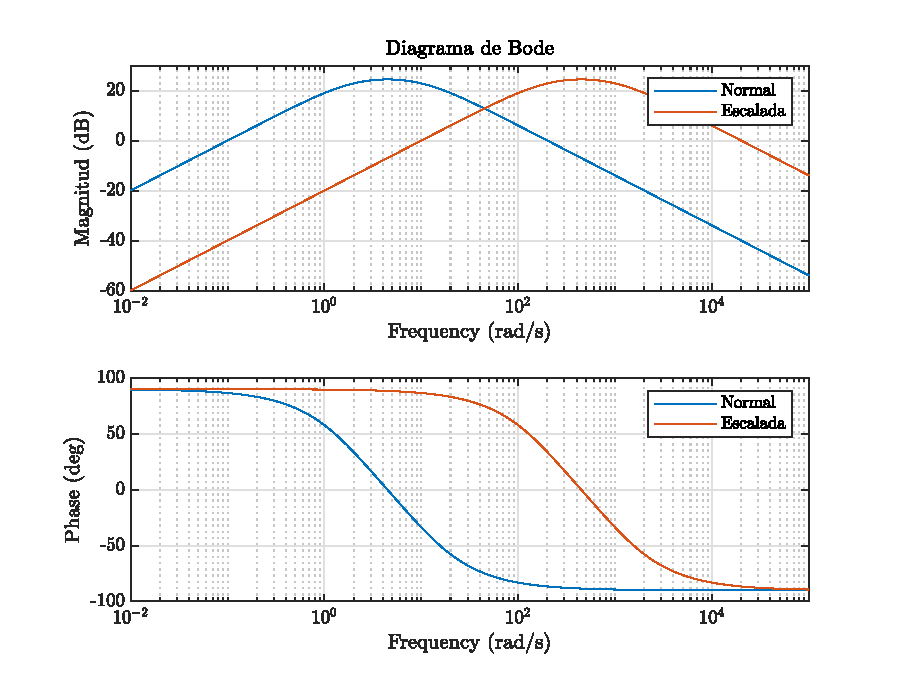
\includegraphics[width=12cm]{F10_bode_escalamiento.eps}
	\end{figure}
	
	\section{Teoría de filtros}
	
	\subsection{Filtros de primer orden}
	
	La función de transferencia general de primer orden esta dada por la siguiente ecuación:
	
	\begin{equation}
	T(s) = \frac{a_{1} s + a_{0} }{s + \omega_{0}}
	\label{ec:bilineal_general}
	\end{equation}
	esta \textbf{función de transferencia bilineal} se caracteriza por tener un polo en $s = - \omega_{0}$, un cero en $s = -\frac{a_{0}}{a_{1}}$ y una ganancia de alta frecuencia que tiende a $a_{1}$. Los coeficientes del numerador, $a_{0}$ y $a_{1}$, determinan el tipo de filtro, ya sea pasabajas (LP), pasaaltas (HP), pasatodas (AP) o general. La realización activa provee considerablemente más versatilidad que su contra parte pasiva, en muchos casos la ganancia puede ser ajustada a un valor deseado, y algunos parámetros de las funciones de transferencia también sin afectar otros. La impedancia de salida de los circuitos activos es muy baja, haciendo que la colocación en cascada sea muy fácil. Sin embargo, los amplificadores operacionales limitan la operación a altas frecuencias de los circuitos activos \cite{Sedra2015}.
	
	Diferentes tipos de filtros nacen de ubicar el cero de la función de transferencia bilineal general (\ref{ec:bilineal_general}) en distintos lugares, un cero en el infinito genera un filtro pasabajas de primer orden, y un cero en el origen un filtro pasaaltas. Las ecuaciones básicas de los filtros de primer orden son las siguientes:
	
	Pasabajas (LP)
	\begin{equation}
	T(s) = \frac{a_{0}}{s + \omega_{0}}
	\end{equation}
	
	Pasaaltas (HP)
	\begin{equation}
	T(s) = \frac{a_{1}s}{s + \omega_{0}}
	\end{equation}
	
	Pasatodas (AP)
	\begin{equation}
	T(s) = -a_{1} \frac{s - \omega_{0}}{s + \omega_{0}}
	\end{equation}
	
	\subsection{Filtros de segundo orden}
	
	La función de transferencia general de un filtro de segundo orden (o \textbf{bicuadrátrica}) se expresa en lo general en la forma estándar:
	
	\begin{equation}
	T(s) = \frac{a_{2} s^{2} + a_{1}s + a_{0}}{s^{2} + \left( \cfrac{ \omega_{0} }{Q} \right)s + \omega_{0}^{2}}
	\end{equation}
	donde $\omega_{0}$ y $Q$ determinan los polos de acuerdo a la siguiente ecuación:
	
	\begin{equation}
	p_{1,2} = - \frac{\omega_{0}}{2 Q} \pm j \omega_{0} \sqrt{1 - \left(   \frac{1}{4 Q^{2}}  \right) \,\,}
	\end{equation}
	al parámetro $\omega_{0}$ se le conoce como la \textbf{frecuencia de polo}, y representa la distancia radial entre el origen y el polo en el plano complejo $s$, a $Q$ se le conoce como el \textbf{factor de calidad de polo} y determina la distancia de los polos desde el eje $j\omega$, una representación gráfica de estos parametros se muestra en la Figura \ref{fig:F11_parametros_Q_w}, entre más grande sea el valor de $Q$, más cerca estarán los polos el eje $j\omega$, y la respuesta del filtro se vuelve más selectiva. Un valor infinito para $Q$ localiza a los polos sobre el eje $j\omega$ y puede producir oscilaciones sostenidas en la realización del circuito. Un valor negativo de $Q$ implica que los polos se encuentran en la mitad derecha del plano s, lo cual ciertamente produce oscilaciones.
	Los ceros del filtro de segundo orden están determinados por los coeficientes del numerador, $a_{0}$, $a_{1}$ y $a_{2}$. Los coeficientes del numerador determinan el tipo de filtro de segundo orden \cite{Sedra2015}.
	
	Para un filtro pasabajas (LP) de segundo orden, los dos ceros están en $s = \infty$ y su respuesta de magnitud muestra un pico para $Q > \frac{1}{\sqrt{2}}$. La respuesta obtenida con $Q = \frac{1}{\sqrt{2}}$ es la respuesta Butterworth o máxima plana. Para un pasaaltas (HP) los ceros están en $s = 0$ y su respuesta de magnitud muestra un pico para $Q > \frac{1}{\sqrt{2}}$. Para un pasabanda (BP) un cero esta en $s = \infty$ y el otro en $s = 0$, la respuesta de magnitud tiene un pico en $\omega = \omega_{0}$, por lo tanto, la \textbf{frecuencia central} del filtro pasabandas es igual a la frecuencia de polo $\omega_{0}$. La selectividad de del filtro pasabanda de segundo orden es usualmente medida por su ancho de banda de 3 dB. Este es la diferencia entre las dos frecuencias $\omega_{1}$ y $\omega_{2}$ en las cuales la respuesta de magnitud es 3 dB por debajo de su valor máximo el cual ocurre en $\omega_{0}$. Las ecuación que describe a las frecuencias $\omega_{1},\omega_{2}$ es la siguiente:
	
	\begin{equation}
		\omega_{1},\omega_{2} = \omega_{0} \sqrt{1 + \left( \frac{1}{4 Q^{2}} \right)}  \pm \frac{\omega_{0}}{2 Q}
	\end{equation}
	Entonces el ancho de banda $BW$ se define como:
	
	\begin{equation}
	BW = \omega_{2} - \omega_{1} = \frac{\omega_{0}}{Q}
	\end{equation}
	\begin{figure}[hbtp]
	\caption{Definición de los parámetros $\omega_{0}$ y $Q$ de un par de polos conjugados.} 
	\label{fig:F11_parametros_Q_w}
	\centering
	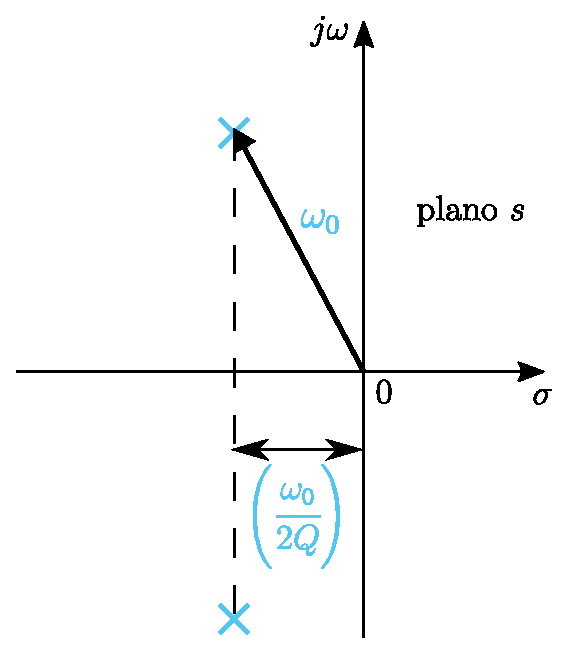
\includegraphics[width=5cm]{F11_parametros_Q_w.eps}
	\end{figure}
	
	Las ecuaciones básicas de filtros de segundo orden son las siguientes:
	
	Pasabajas (LP)
	\begin{equation}
	T(s) = \frac{a_{0}}{s^{2} + \cfrac{\omega_{0}}{Q} s + \omega_{0}^{2}}
	\end{equation}
	
	Pasaaltas (HP)
	\begin{equation}
	T(s) = \frac{a_{2} s^{2}}{s^{2} + \cfrac{\omega_{0}}{Q} s + \omega_{0}^{2}}
	\end{equation}
	
	Pasabandas (BP)
	\begin{equation}
	T(s) = \frac{a_{1} s}{s^{2} + \cfrac{\omega_{0}}{Q} s + \omega_{0}^{2}}
	\end{equation}
	
	Pasatodas (AP)
	\begin{equation}
	T(s) = a_{2} \frac{s^{2} - \cfrac{\omega_{o}}{Q}s + \omega_{0}^{2} }{s^{2} + \cfrac{\omega_{0}}{Q} s + \omega_{0}^{2}}
	\end{equation}
	
	\chapter{Implementación}

	\section{¿Qué es una FPAA?}
	Una FPAA  por sus siglas en inglés (Field Programmable Analog Arrays) es un dispositivo analógico equivalente a las FPGA (Field Programmable Garte Arrays). A diferencia de las FPGA que contienen una gran cantidad de módulos y conexiones que permiten configuraciones arbitrarias de lógica combinacional y secuencial, los FPAA generalmente contienen una pequeña cantidad de CABs (Configurable Analog Blocks). Los FPAA dirigidos al diseño analógico estándar generalmente presentan un CAB que contiene un amplificador operacional, un arreglo de capacitores programables, y ya sea un arreglo de resistencias programables para circuitos en tiempo continuo o switches configurables para circuitos de capacitores conmutados.
	Se trabajó con la tarjeta Anadigm QuadApex Develovment Boarsd v2.0 de la empresa Anadigm, la cual contiene 4 FPAAs AN231E04 que pueden conectarse en cadena y es programada mediante el software AnadigmDesigner2 (AD2). El diagrama esquemático de la tarjeta se puede ver en la Figura \ref{fig:esquematico_fpaa} del apéndice.
	
	\section{Características de la tarjeta y requerimientos}
	
	\subsection{Alimentación de la tarjeta}
	Para el correcto funcionamiento de la placa esta debe ser alimentada con una fuente de voltaje regulada a 5V de al menos 500mA conectada a la clema de dos terminales. Hay un LED de color verde que indica que la placa se ha encendido correctamente, la placa esta protegida contra la conexión de una fuente de voltaje con la polarización incorrecta.
	
	\subsection{Instalación de drivers}

No conecte la placa QuadApex v2.0 a la PC vía cable USB,  ni tampoco inicie AD2 ahora, el driver debe instalarse primero. Se asume que AD2 ya ha sido instalado y registrado en su computadora, de lo contrario entre al link que aparece a continuación.

Para instalar AD2 basta con acceder al siguiente link y seguir los pasos que muestra la pagina:

	\begin{center}
		\url{https://www.anadigm.com/sup_downloadcenter.asp?tab=ad2}
	\end{center}
es recomendable guardar los datos de registro en un lugar seguro, al iniciar el programa por primera vez es necesario ingresar el \textbf{License ID} y la \textbf{License key} estos estarán en el correo que le proporcionó a Anadigm. 

El driver \textbf{CP210x\_{}Drivers.exe} está incluido en el AD2 CD o se puede encontrar en la página de Silicon Labs. Siga los siguientes pasos si es la primera vez que instala este driver, de lo contrario desinstale las versiones anteriores antes de continuar:

\begin{enumerate}
	\item Ejecute como administrador el ejecutable  CP210x\_{}Drivers.exe. El destino por defecto del ejecutable es ‘‘C:\textbackslash{}Silabs\textbackslash{}Mcu\textbackslash{}CP210x’’.
	\item Para completar la instalación conecte la QuadApex v2.0 y enciéndala.
	\item Acceda al administrador de dispositivos y en \textbf{Puertos (COM y LPT)} asegúrese que el driver este bien configurado, si no aparece un signo de admiración y se le asigno un puerto COM  la instalación fue exitosa, de lo contrario dar clic derecho sobre el dispositivo y seleccionar \textbf{Actualizar controlador}, después buscar el  driver en la ruta del paso 1.
\end{enumerate}

El driver en este punto ya esta instalado. La instalación del driver y la asignación del puerto es necesaria solo una vez. Si se conecta subsecuentemente a otro puerto de USB de la PC puede ser necesario repetir el paso 3.

	
	\subsection{Jumpers por defecto}
	
	En la Tabla \ref{tab:jumpers} se muestra una lista con los jumpers que contiene la placa, una descripción de su funcionamiento y su posición por defecto. Es importante colocar la FPAA con todos sus jumper en el estado por defecto para entender secciones posteriores y evitar errores. La placa no contiene una cantidad muy grande de jumpers y usualmente solo se modificarán los jumpers J8,9,10, los cuales son los que controlan la cantidad de FPPAs activas.
	
\begin{table}[!ht]
		\centering
		\caption{Resumen de jumper de la placa.}
		\label{tab:jumpers}
		\resizebox{15cm}{!} {
		\begin{tabular}{|p{1.7cm}|p{9.5cm}|p{4.5cm}|p{5.5cm}|}
			\hline
			\textbf{Jumper} &  \textbf{Función} & \textbf{Estado por defecto}	& 	\textbf{Condición por defecto}\\
			\hline
			J1		&	Conecta la sección digital a la sección analógica.	&	Todos los 13 jumpers deben estar conectados &	Conecta completamente la alimentación, tierra y todas las señales digitales FPAA a la sección digital.\\
			\hline
			J2		&	Selecciona entre 16MHz y 40MHz para la fuente ACLK. &	Jumpers off &	ACLK$=$16MHz\\
			\hline
			J3		& Permite la descarga de la configuración de prueba a todos los FPAA desde FLASH (después de reiniciar o apagar y encender). El circuito de prueba despliega ondas sinusoidales a todas las salidas FPAA. &	Jumper off	& Descarga del circuito de prueba deshabilitado\\
			\hline
			J4		& Permite el almacenamiento de configuraciones primarias en el FLASH del PIC32 si el puente está activado. & Jumper off		&	No en modo de almacenamiento de configuraciones primarias.\\
			\hline
			J5		& Jumper de repuesto.	&	Jumper off &	-\\
			\hline
			J6		& Un jumper en J5 deshabilitará el módulo oscilador de 16MHz y tristateará su salida. Esto significa que el pin ACLK de los FPAA no se sincronizará, tampoco se sincronizará el microcontrolador PIC32, por lo que toda la placa se desactivará efectivamente. & Jumper off	& Oscilador de 16MHz habilitado	\\
			\hline
			J7		& Este jumper controla la generación de un suministro negativo (-3.3V) para las etapas del buffer de salida en la placa. El puente a la derecha desactiva el suministro negativo (lo ata al suelo). El puente a la izquierda permite el suministro.	& Jumper a la izquierda	&	Alimentación negativa habilitada\\
			\hline
			J8,9,10	& Estos jumpers en combinacion con ACT1, ACT2, ACT3, ACT4 controlan la cadena de FPAAs.	& Todos los jumpers especificados deben estar conectados	& Todas las FPAA en cadena	\\
			\hline
			J11		& Estos jumpers conectan el transceptor USB a la interfaz UART del microcontrolador PIC32. Si no se requiere control USB, estos 4 puentes se pueden quitar.	& Todos los jumpers conectados	& USB habilitado 	\\		
			\hline
		\end{tabular}
		}
\end{table}

	\subsection{Tamaño variable de cadena de FPAAs}

	La placa contiene 4 FPAAs en cadena. Esta cadena puede ser cortada a 3, 2 o 1, pero debe ser cortada deshabilitando FPAAs desde el final de la cadena (del lado derecho).

\begin{itemize}
	\item Pare reducir la cadena a 3 FPAAs, remueva los jumpers de \textbf{J10} y también el jumper marcado \textbf{ACT4} de \textbf{J1}. Esto deshabilitará FPPAA \#4 (la más cercana a la fuente de alimentación.)
	\item Para reducir la cadena a 2 FPAAs, remueva los jumpers de \textbf{J9} y \textbf{J10} y también los jumpers marcados \textbf{ACT3} y \textbf{ACT4} de \textbf{J1}. Esto deshablitará los FPAAs \#3 y \#4.
	\item Para reducir la cadena a 1 FPAA, remueva los jumpers de \textbf{J8, J9} y \textbf{J10} y  también los jumpers marcados \textbf{ACT2, ACT3} y \textbf{ACT4} de \textbf{J1}. Esto deshabilitará los FPAA \#2, \#3 y \#4.
\end{itemize}
\textbf{Nota:} si se configura una cadena de FPAA y luego se desconectan 1 o más FPAA de la cadena, los FPAA desconectados aún mantendrán su configuración hasta que se reinicie la placa o se vuelva a configurar la cadena (reducida).

	\subsection{DIP Switches}
	
	El usuario puede hacer sus propias conexiones en la placa con cables, pero hay un conjunto de DIP switches que permiten una fácil conexión de ciertas rutas entre los FPAA vecinos y entre los FPAA y los \textbf{input/output buffers}. Estos interruptores están abiertos por defecto, lo que significa que todos están hacia la izquierda. El usuario puede cerrar los interruptores empujándolos hacia la derecha. En la Tabla \ref{tab:switches} se muestra un resumen de los switches. Los DIP switches son pequeños y del tipo deslizantes, por lo que se recomienda una herramienta afilada como un destornillador delgado para abrir y cerrar los switches. Algunos ejemplos se muestran a continuación:
	
	\begin{enumerate}
		\item Para conectar el filtro Rauch\_\#1\_I01 a I1 de la FPPA\#{}1, cierre los 4 interruptores en S10.
		\item Para conectar O4 del FPAA\#{} a I1 del FPAA\#{}2, cierre los 2 interruptores superiores de S2.
		\item Para conectar O3 del FPAA\#{}1 al buffer de salida BUF\_\#1\_03, cierre ambos switches de S13.
	\end{enumerate}

	\begin{table}[!ht]
		\centering
		\begin{tabular}{|l|l|l|}
			\hline
			\textbf{Función} &  \textbf{Tipo} & \textbf{Labels}\\
			\hline
			Conectar filtros Rauch a entradas de FPAA 					& 4way 		& S8,9,10,11,15,16,17,18		\\
			\hline
			Conectar entre FPAAs 						& 4way 	& S2,3,4,5,6,7	\\
			\hline
			Conectar FPAA a buffers de salida 						& 2way 		& S12,13,14,19		\\
			\hline
		\end{tabular}
		\caption{DIP Switches}
		\label{tab:switches}
	\end{table}

	\subsection{Filtros Rauch y buffers de salida}
	
	La tarjeta cuenta con 2 buffers de entrada llamados filtros Rauch listos para usar, \textbf{Rauch\_\#1\_I01} y \textbf{Rauch\_\#2\_I01}, estos son filtros multipropósito cuya su principal función es convertir una señal single-ended a una diferencial en la FPAA, internamente la FPAA trabaja únicamente con señales diferenciales y debido a esto el uso de estos filtros es imprescindibles para introducir señales externas, por ejemplo de generadores de funciones u otros circuitos. Si se usa una señal single-ended, es necesario conectar IN- a GND y conectar la señal en IN+.
	Para activar el filtro es necesario hacerlo desde el software AD2 haciendo doble clic en la IO cell apropiada (IOCell1-4), seleccionar Input y después Amplifier, esto es debido a que el filtro funciona en combinación con un amplificador integrado en la FPAA y los componentes pasivos de montaje superficial que vienen soldados de fabrica.
	
	Rauch\_\#1\_I01 está conectado a I/O1 de la FPAA \#1 y esta configurado con una frecuencia de corte muy alta y ganancia unitaria ($F_{o} = 490$KHz). Rauch\_\#21\_I01 está conectado a I/O1 de la FPAA \#2 y esta configurado con una ganancia unitaria y una frecuencia de corte de poco más de 20kHz, que es típica de una aplicación de audio. 

	La tarjeta también cuenta con 2 buffers de salida listos para usar, \textbf{Buf\_\#1\_O3} y  \textbf{Buf\_\#2\_O3}, cuyo principal propósito es convertir la salida diferencial de la FPAA a una single-end. 
	Buf\_\#1\_O3 está conectado a O3 de la FPAA \#1 y está configurado con una frecuencia de corte muy alta y una ganancia unitaria. Si se requiere una frecuencia de corte inferior, es muy fácil modificar este filtro sin quitar los componentes de montaje superficial debajo, simplemente agregando capacitores TH. Buf\_\#2\_O3 está conectado a O3 de FPAA \#2 y esta configurado con una ganancia unitaria y una frecuencia de corte de poco más de 20 kHz, que es típica de una aplicación de audio. 
	
	Cabe resaltar que para utilizar tanto los filtros Rauch como los buffers de salida sin cables adicionales es necesario cerrar los DIP switches correspondientes, no obstante se pueden cablear externamente a cualquiera de las entradas o salidas de las FPAA.
	
	\subsection{Circuito de prueba}

La placa es capaz de autoconfigurar los FPAAs con un circuito de prueba para una verificación rápida de la placa. Para hacer esto, coloque un jumper en \textbf{J3} y reinicie la placa. Todos los FPAA en la cadena ahora se configurarán con el circuito de prueba (el LED verde indica que la configuración fue exitosa). Este circuito de prueba genera una onda sinusoidal en todas las 7 salidas del FPAA (14 salidas diferenciales). La frecuencia de esta onda sinusoidal es de 1kHz en FPAA \#{}1, 2kHz en FPAA \#{}2, 4kHz en FPAA \#{}3 y 8kHz en FPAA \#{}4. Si se habilitan menos de 4 FPAA en la cadena, solo se configurarán aquellos FPAA que estén habilitados. Si se coloca un jumper en \textbf{J3} y \textbf{J4}, se cargará un circuito diferente en los FPAAs. Este es un circuito de prueba especial utilizado por Anadigm durante la producción. Se aconseja al usuario que no coloque jumpers en J3 y J4 al mismo tiempo.

	\section{AnadigmDesigner2}
	
	AD2 trabaja con módulos llamados CAMs (Configurable Analog Modules), estos aportan flexibilidad y sencillez en el proceso diseño debido a que son bloques que hacen desde funciones sencillas como inversores o comparadores hasta diseños completos como filtros y multiplicadores. Los CAMs pueden interconectarse fácilmente unos con otros y únicamente necesitan pequeñas configuraciones para su correcto funcionamiento. Los CAMs más utilizados son los mostrados en la Tabla \ref{tab:CAMs_AD2}. En secciones posteriores se abordará con más detalle como configurarlos y cuales son las ecuaciones necesarias para calcular los parámetros de cada uno.  
	

\begin{table}[!ht]
  \centering
  \caption{CAMs básicos de AD2.}
  \label{tab:CAMs_AD2}
  \begin{tabular}{>{\centering\arraybackslash}m{3cm} >{\centering\arraybackslash}m{5cm} >{\centering\arraybackslash}m{5cm}}
    \hline
    \textbf{Nombre} & \textbf{Función de transferencia} & \textbf{Descripción}\\ 
    \hline
    {\scriptsize \textbf{GainInv}}
    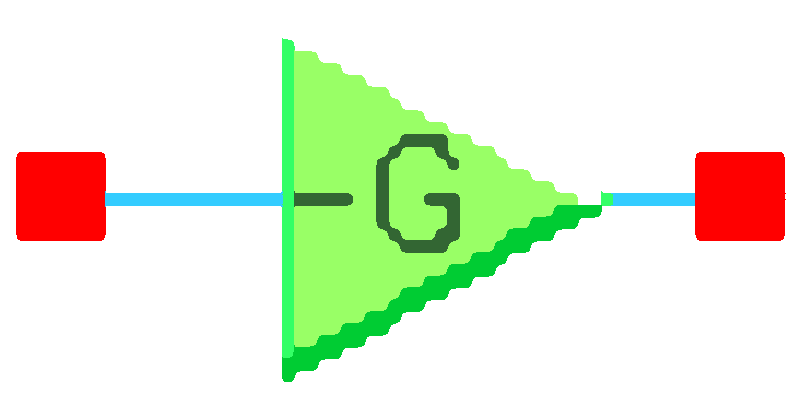
\includegraphics[width=2.2cm]{T7_Inversor.eps}
    &
      $\frac{V_{\mathrm{out}} (s)}{V_{\mathrm{in}}(s)} = - G$
    & 
      \begin{itemize}[leftmargin=0cm,noitemsep]
      \begin{scriptsize}
		\item[] Ganancia inversora.
		\item[] Gain: 0.01 - 100.0 V/V
      \end{scriptsize}
      \end{itemize}
    \\ %-------------------------------------------------------
    {\scriptsize \textbf{Integrator}}
    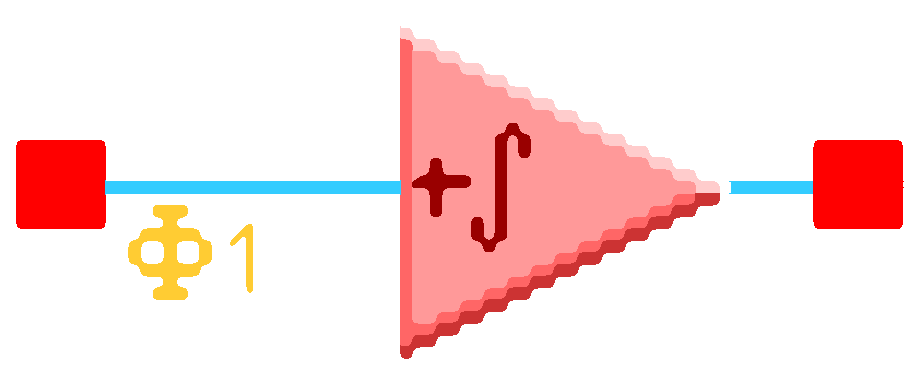
\includegraphics[width=2.5cm]{T1_Integrador.eps}
    &
      $ \frac{V_{\mathrm{out}} (s)}{V_{\mathrm{in}}(s)} = \frac{\pm K}{s}$
    & 
      \begin{itemize}[leftmargin=0cm,noitemsep]
      \begin{scriptsize}
		\item[] Integrador con una constante de integración programable. La salida puede ser inversora o no inversora.
      \end{scriptsize}
      \end{itemize}
    \\ %-------------------------------------------------------
    {\scriptsize \textbf{Voltage}} \linebreak
    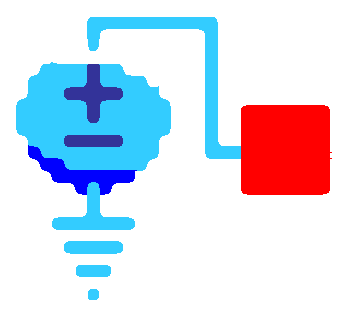
\includegraphics[width=1cm]{T6_DC_voltage.eps}
    &
      $V_{\mathrm{out}} = \pm 2$
    & 
      \begin{itemize}[leftmargin=0cm,noitemsep]
      \begin{scriptsize}
		\item[] Referencia de voltaje de $\pm$ 2 V.
      \end{scriptsize}
      \end{itemize}
    \\ %-------------------------------------------------------
    {\scriptsize \textbf{TransferFunction}} \linebreak
    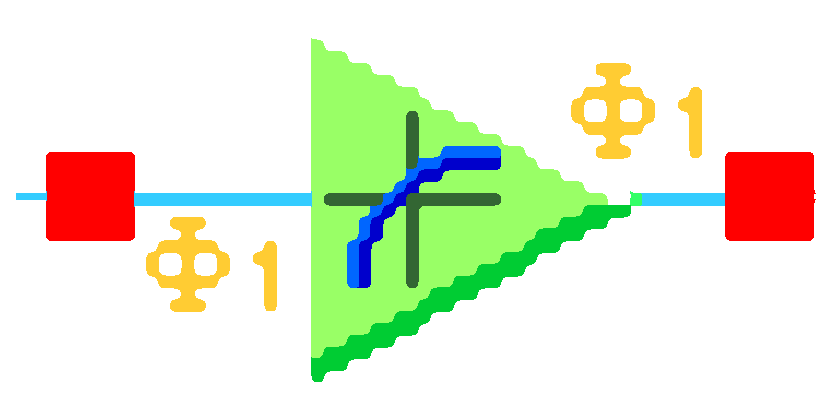
\includegraphics[width=2.5cm]{T3_Transferfunction.eps}
    &
    & 
      \begin{itemize}[leftmargin=0cm,noitemsep]
      \begin{scriptsize}
		\item[] \textbf{Lookup Table}: función de transferencia especificada por el usuario de 256 de pasos de cuantificación.  
      \end{scriptsize}
      \end{itemize}
    \\ %-------------------------------------------------------
    {\scriptsize \textbf{Multiplier}} \linebreak
    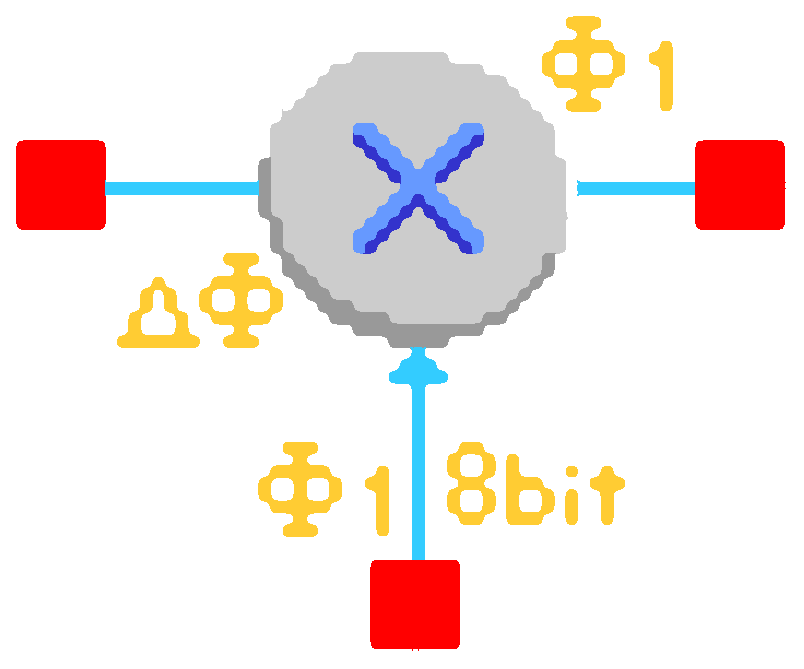
\includegraphics[width=2.5cm]{T2_Multiplicador.eps}
    &
      $V_{\mathrm{out}} = M \cdot V_{x} \cdot V_{y}$
    & 
      \begin{itemize}[leftmargin=0cm,noitemsep]
      \begin{scriptsize}
		\item[] $V_{x}$ es la entrada de voltaje izquierda.
		\item[] $V_{y}$ es la entrada de voltaje inferior cuantificado de 8 bits.
		\vspace{-0.15cm}
		\item[] $M$ factor de multiplicación.
      \end{scriptsize}
      \end{itemize}
    \\ %-------------------------------------------------------
    {\scriptsize \textbf{SumDiff}} \linebreak
    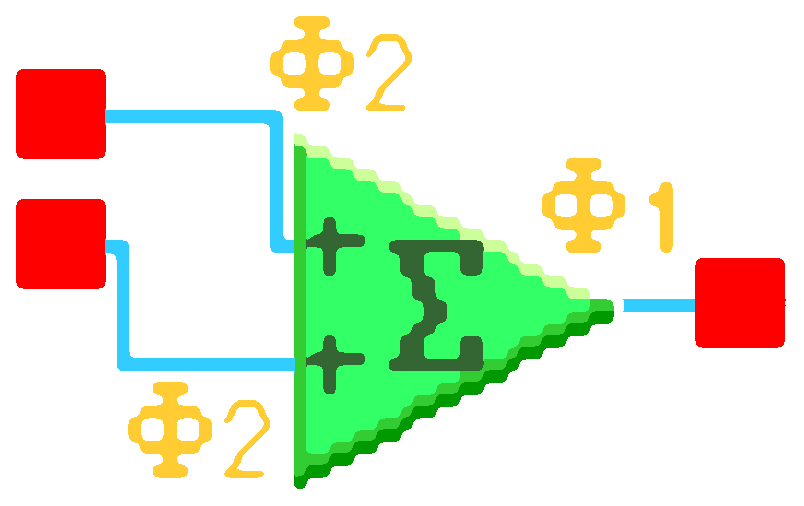
\includegraphics[width=2.5cm]{T8_Sumador.eps}
    &
      \begin{footnotesize}
      	$V_{\mathrm{out}} = \pm G_{1} V_{\mathrm{in1}} \pm G_{2} V_{\mathrm{in2}} \pm G_{3} V_{\mathrm{in3}} \pm G_{4} V_{\mathrm{in4}}$
      \end{footnotesize}
    & 
      \begin{itemize}[leftmargin=0cm,noitemsep]
      \begin{scriptsize}
		\item[] Las entradas pueden ser inversoras o no inversoras.
		\item[]	Cada entrada tiene una ganancia programable.
		\vspace{-0.15cm}
		\item[] Configurable desde 2 hasta 4 entradas. 
      \end{scriptsize}
      \end{itemize}
    \\ %-------------------------------------------------------
    {\scriptsize \textbf{FilterBilinear}} \linebreak
    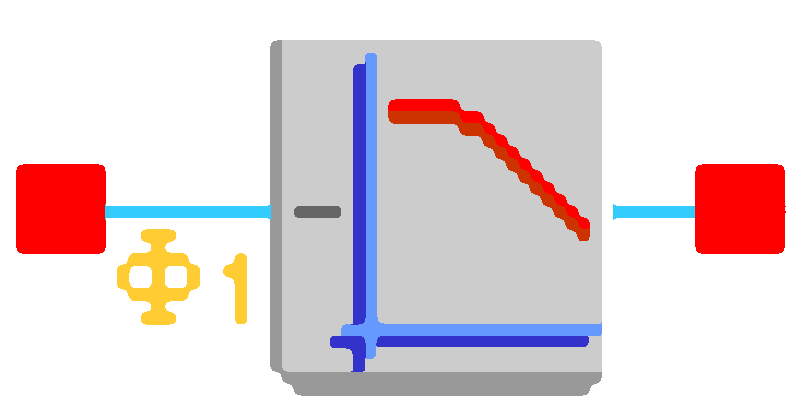
\includegraphics[width=2.5cm]{T9_FilterBilinear.eps}
    &
      \begin{scriptsize}
		 \textbf{Low Pass Bilinear Filter} \linebreak
      	 $\frac{V_{\mathrm{out}}(s)}{V_{\mathrm{in}}(s)} = \pm \frac{2 \pi f_{0} G}{s + 2 \pi f_{0}}$ \linebreak
      	 \textbf{High Pass Bilinear Filter} \linebreak
      	 $\frac{V_{\mathrm{out}}(s)}{V_{\mathrm{in}}(s)} = - \frac{Gs}{s + 2 \pi f_{0}}$ \linebreak
      	 $\vdots$
      \end{scriptsize}
    & 
      \begin{itemize}[leftmargin=0cm,noitemsep]
      \begin{scriptsize}
		\item[] Puede ser configurado como pasabajas, pasaaltas, pasatodas o general (Polo y cero).
      \end{scriptsize}
      \end{itemize}
    \\ %-------------------------------------------------------
    {\scriptsize \textbf{FilterBiquad}} \linebreak
    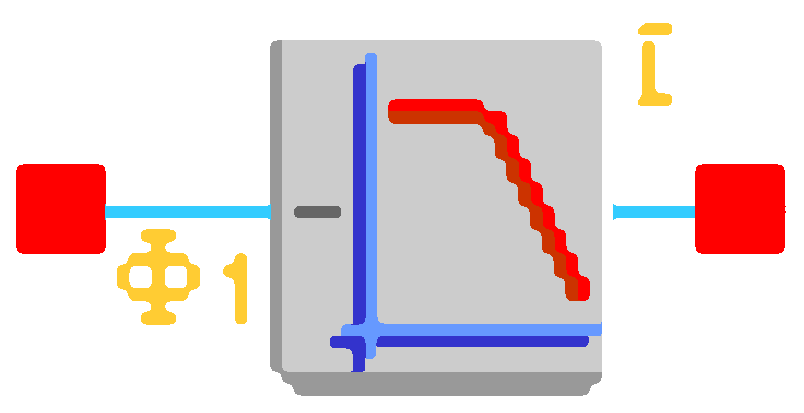
\includegraphics[width=2.5cm]{T10_FilterBiquad.eps}
    &
      \begin{scriptsize}
		 \textbf{Low Pass Biquadratic Filter} \linebreak
      	 $\frac{V_{\mathrm{out}}(s)}{V_{\mathrm{in}}(s)} = \frac{\pm 4 \pi^{2} f_{0}^{2} G}{s^{2} + \frac{2 \pi f_{0}}{Q}s + 4 \pi^{2} f_{0}^{2}}$ \linebreak
      	 \textbf{High Pass Biquadratic Filter} \linebreak
      	 $\frac{V_{\mathrm{out}}(s)}{V_{\mathrm{in}}(s)} = \frac{-G s^{2}}{s^{2} + \frac{2 \pi f_{0}}{Q} s + 4 \pi^{2} f_{0}^{2}}$ \linebreak
      	 $\vdots$
      \end{scriptsize}
    & 
      \begin{itemize}[leftmargin=0cm,noitemsep]
      \begin{scriptsize}
		\item[] Puede ser configurado como pasabajas, pasaaltas, pasabanda, rechazabanda o general (Polos y ceros).
      \end{scriptsize}
      \end{itemize}
    \\ %-------------------------------------------------------
    \hline
  \end{tabular}
\end{table}
	
	\subsection{Comunicación con AD2}

Ahora la placa puede ser programada lo que en este caso significa configurar los FPAA. Esto puede realizarse desde una PC o una laptop usando un cable estándar USB tipo A-B. La placa usa una emulación de comunicación serial de tal manera que  desde la computadora la placa aparecerá como un puerto COM.

Para programar la placa conecte el cable USB entre la placa y la computadora y encienda la placa. Abra AD2 y haga clic en \textbf{Settings/Preferences}, después haga clic en la pestaña \textbf{Port}. En el menú desplegable \textbf{Select Port} debe estar el puerto COM correspondiente a la placa Anadigm. Este es en realidad un puerto COM virtual porque la placa tiene un \textbf{USB/UART bridge} llamado CP2102 el cual emula un puerto serial. 

Seleccione el puerto COM correspondiente. Haga clic en \textbf{Apply}, después en \textbf{OK}. Para comprobar que AD2 ahora puede comunicarse con la placa, haga clic en \textbf{Target/Display Board Information}. El LED verde D4 se apagará.

\begin{figure}[hbtp]
\caption{Información de la placa desplegada por AD2.}
\label{fig:G1_AD2_board_info.png}
\centering
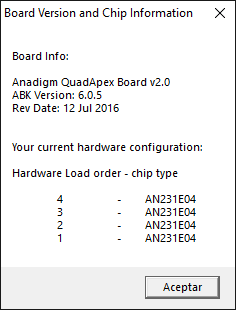
\includegraphics[width = 5cm]{G1_AD2_board_info.png}
\end{figure}
	
	La Figura \ref{fig:G1_AD2_board_info.png} muestra la información que despliega AD2 acerca de la placa donde todas las 4 FPAA están configuradas en cadena. Si menos FPAA están configuradas entonces la información de la placa mostrará cuantas FPAA están disponibles.

Ahora debería ser posible descargar un circuito desde AD2. Para hacer esto simplemente se da clic sobre el icono de descarga (a la izquierda del signo de interrogación, debajo de Dynamic Config). Como alternativa presiona \textbf{Ctrl + W}. Un LED amarillo comenzará a parpadear mientras cada FPAA es configurada y finamente un LED verde se encenderá indicando que todas las FPAA han sido configuradas correctamente. Un LED rojo indicará que la configuración falló. Es importante que el número de FPPA en AD2 coincida con el número de FPAA habilitadas en la placa. Por ejemplo, si la tarjeta fue configurada con una cadena de 3 FPAA, entonces estará esperando 3 configuraciones de FPAA para ser descargadas desde AD2.
	
	
	\subsection{Configuración de relojes}
	
	Las configuraciones de los CAMs dependen de las frecuencias de reloj que se seleccionen para cada FPAA. Cada FPAA tiene dos fuentes de frecuencias de reloj de sistema \textbf{Sys1} y \textbf{Sys2}, y seis frecuencias de reloj de chip, desde \textbf{Clock 0} hasta \textbf{Clock 5} que son subdivisiones de cualquiera de las fuentes de reloj sistema. Seleccionar y configurar correctamente los relojes es importante ya que el rango de operación de los CAMs depende de esto. 
	
\begin{figure}[!hbp] 
\caption{Ventana de configuración de frecuencias de reloj AD2.}
\label{fig:G3_Frecuencias_AD2.png}
\centering
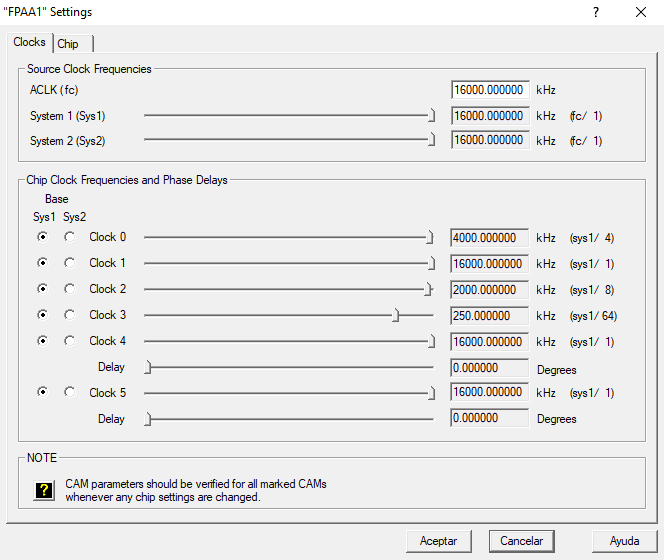
\includegraphics[width = 12cm]{G3_Frecuencias_AD2.png}
\end{figure}

La tarjeta tiene una fuente de frecuencia de reloj principal llamada \textbf{ACLK} o $f_{c}$ cuya frecuencia es igual a $16$ MHz y no puede ser cambiada. Sys1 y Sys2 dependen de esta frecuencia y pueden ser modificadas utilizando las siguientes ecuaciones:

\begin{equation}
\mathrm{Sys1} = \frac{f_{c}}{m} \qquad \mathrm{Sys2} = \frac{f_{c}}{m}
\label{ec:sys_clock}
\end{equation}
donde $m\in [1,510]$ y es par. Usualmente Sys1 y Sys2 no se modifican pero es necesario entender que estas dos fuentes de frecuencias de reloj a su vez controlan a las fuentes de reloj de chip desde \textbf{Clock 0} hasta \textbf{Clock 5} dada la siguiente ecuación:

\begin{equation}
	\mathrm{Clock\,} h = \frac{\mathrm{Sys1}}{n}	\qquad   \mathrm{Clock\,} h = \frac{\mathrm{Sys2}}{n}
	\label{ec:clock_h}
\end{equation}
donde $n\in[1,510]$ y es par y $h\in[0,5]$. Configurar las fuentes de reloj de chip cobrará importancia en secciones posteriores y las ecuaciones anteriores no deben olvidarse.
	\section{Implementación con aproximación de primer orden}
	
	Para realizar la implementación física de la aproximación de primer orden del integrador fraccionario se utilizó el CAM \textbf{FilterBilinear} en su modo \textbf{Pole and Zero}, esto debido a su flexibilidad y semejanza con la función de transferencia de la aproximación de la CFE de primer orden. La función de transferencia del CAM en este modo es la siguiente:
	
	\begin{equation}
		\frac{V_{\mathrm{out}} (s)}{V_{\mathrm{in}}(s)} = -\frac{G_{H} (s + 2 \pi f_{z})}{s + 2 \pi f_{p}}
		\label{ec:CAM_bilineal}
	\end{equation}
	donde $G_{L}$ esta definida como:
	\begin{equation}
		G_{L} = \frac{f_{z}}{f_{p}} G_{H}
	\end{equation}
	y donde $G_{L}$ es la ganancia en DC, $G_{H}$ es la ganancia de alta frecuencia, $f_{p}$ es la frecuencia del polo y $f_{z}$ es la frecuencia del cero. Si se utiliza un CAM de ganancia inversora (\textbf{GainInv}) se puede prescindir del signo negativo de la ecuación (\ref{ec:CAM_bilineal}).
	
	La función de transferencia de la aproximación con la CFE de primer orden, como se mencionó anteriormente es la siguiente:
	\begin{equation}
		\genfrac{}{}{0pt}{0}{}{_{(c_{2})}} \frac{1}{s^{\alpha}} \approx \frac{(1 - \alpha)s + (1 + \alpha) }{(1 + \alpha)s + (1 - \alpha)} 
		\label{ec:cfe_primer_orden}
	\end{equation}
	si consideramos la siguiente sustitución:
	
	\begin{equation}
		A = \frac{1 - \alpha}{1 + \alpha}
	\end{equation}
	podemos reescribir la ecuación (\ref{ec:cfe_primer_orden}) de la siguiente manera:
	
	\begin{equation}
		\genfrac{}{}{0pt}{0}{}{_{(c_{2})}} \frac{1}{s^{\alpha}} \approx \frac{A s + 1}{s + A}
		\label{ec:cfe_primer_orden_simp}
	\end{equation}
	no obstante el ancho de bando de la ecuación (\ref{ec:cfe_primer_orden_simp}) es de $10^{-1}$ rad/s hasta $10^{1}$ rad/s, ver Figura \ref{fig:F10_bode_escalamiento}, lo cual es un rango de frecuencias muy bajo y presenta dificultades en su implementación. Por  esta razón se opta por aplicar un escalamiento en frecuencia a la ecuación (\ref{ec:cfe_primer_orden_simp}) utilizando los siguiente pasos: 
	
	\begin{enumerate}
		\item Cambiamos la variable compleja por $p$ la cual representa la frecuencia actual:
			\begin{equation}
				N(p) =  \frac{A p + 1}{p + A}
			\end{equation}
		\item Utilizamos la sustitución $p = \cfrac{s}{k_{f}}$:
			\begin{equation}
				N(s) =  \frac{A s k_{f}^{-1} + 1}{s k_{f}^{-1} + A}
			\end{equation}
		\item Reescribimos de una manera más conveniente:
			\begin{equation}
				\genfrac{}{}{0pt}{0}{}{_{(c_{2})}} \frac{1}{s^{\alpha}} \approx \frac{A s + k_{f}}{s + A k_{f}}
				\label{ec:cfe_primer_orden_simp_esc}
			\end{equation}
	\end{enumerate}		
	El factor de escalamiento $k_{f}$ se puede elegir a conveniencia dependiendo del ancho de banda necesario, no obstante la frecuencia de entrada de la mayoría de los CAM esta limitada aproximadamente a valores menores de 2 MHz, esto debido a que el tipo de procesamiento de señal del CAM se basa en arquitecturas de datos muestreados. Por esta razón se opta por un escalamiento con un factor $k_{f} = 2\pi 1000$. En la Figura \ref{fig:F12_bode_1er_orden_escalado.eps} se muestra el resultado de aplicar el escalamiento. El nuevo ancho de banda abarca desde $100$ Hz hasta $10$ kHz el cual se encuentra dentro del rango de operación de los CAMs.
	
\begin{figure}[hbtp]
\caption{Diagrama de bode de ecuación (\ref{ec:cfe_primer_orden_simp_esc}) para un integrador fraccionario con $k_{f} = 2\pi 1000$ y  $\alpha = 0.5$.} 
\label{fig:F12_bode_1er_orden_escalado.eps}
\centering
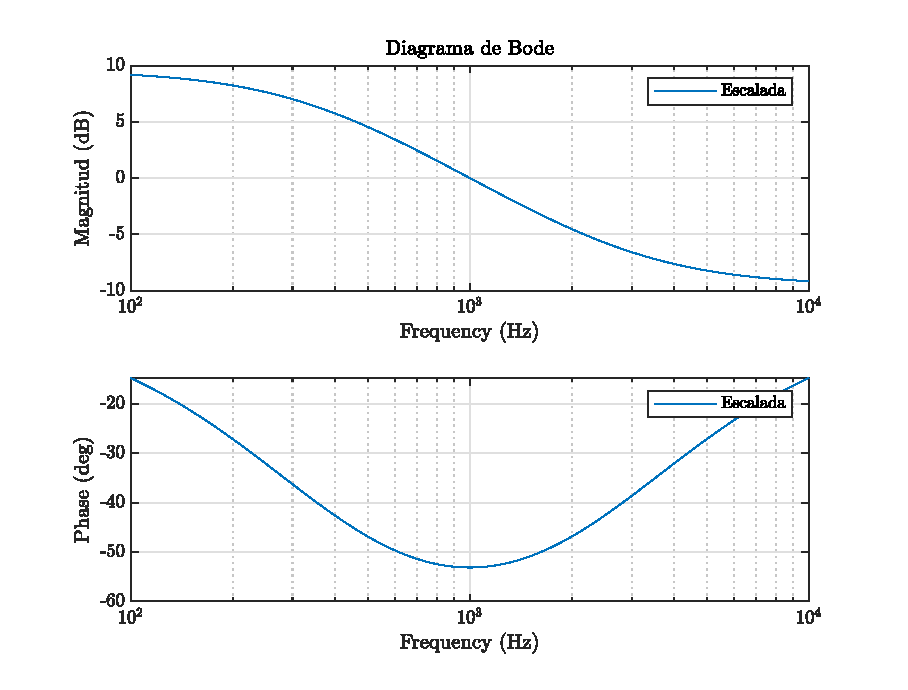
\includegraphics[width=12cm]{F12_bode_1er_orden_escalado.eps}
\end{figure}
	
	 Para poder configurar el CAM FilterBilinear es necesario encontrar los valores correctos para los parámetros $G_{H}$, $G_{L}$, $f_{z}$ y $f_{p}$ dado un orden $\alpha$, y esto se logra igualando las ecuaciones (\ref{ec:cfe_primer_orden_simp_esc}) y (\ref{ec:CAM_bilineal}) con el fin de encontrar expresiones para calcularlos.
	 
	 \begin{equation}
	 \frac{G_{H}(s + 2 \pi f_{z})}{s + 2 \pi f_{p}} = \frac{As + k_{f}}{s + A k_{f}}
	 \label{ec:igualar_bilineal}
	 \end{equation}
	 de la ecuación (\ref{ec:igualar_bilineal}) se deducen las siguientes ecuaciones:
	 
	 \begin{equation}
		 G_{H} = A
		 \label{ec:bilineal_gh}
	 \end{equation}
	 
	 \begin{equation}
	 	f_{p} = \frac{A k_{f}}{2 \pi}
	 	\label{ec:bilineal_fp}
	 \end{equation}
	 
	 \begin{equation}
		f_{z} = \frac{k_{f}}{ 2A \pi}
		\label{ec:bilineal_fz}
	 \end{equation}
	 
	 \begin{equation}
	 G_{L} = \frac{1}{A}
	 \label{ec:bilineal_gl}
	 \end{equation}
	utilizando las ecuaciones anteriores y considerando $k_{f} = 2 \pi 1000$ obtenemos los datos de la Tabla \ref{tab:calculos_bilineal}, esta tabla se puede generar utilizando el código del apéndice \ref{cod:A10_calculo_valores_FilterBilienar}, sin embargo debido a que el CAM FilterBilinear depende directamente de la frecuencia de reloj que se seleccione en el parámetro \textbf{ClockA} no todos los valores de la tabla pueden ser ingresados, en la ventana de configuración aparecerán marcados en color rojo, por lo tanto  es necesario hacer un análisis de frecuencias para este parámetro. En la ventana de configuración del CAM, ver Figura \ref{fig:G2_FilterBilinear_config.png}, se pueden ingresar 3 de los 4 parámetros requeridos, el parámetro restante es calculado automáticamente. Por simplicidad se eligió que el parámetro que se calcule automáticamente sea \textbf{DC Gain}. 
	   
\begin{figure}[!ht] 
\caption{Ventana de configuración de parámetros FilterBilinear.}
\label{fig:G2_FilterBilinear_config.png}
\centering
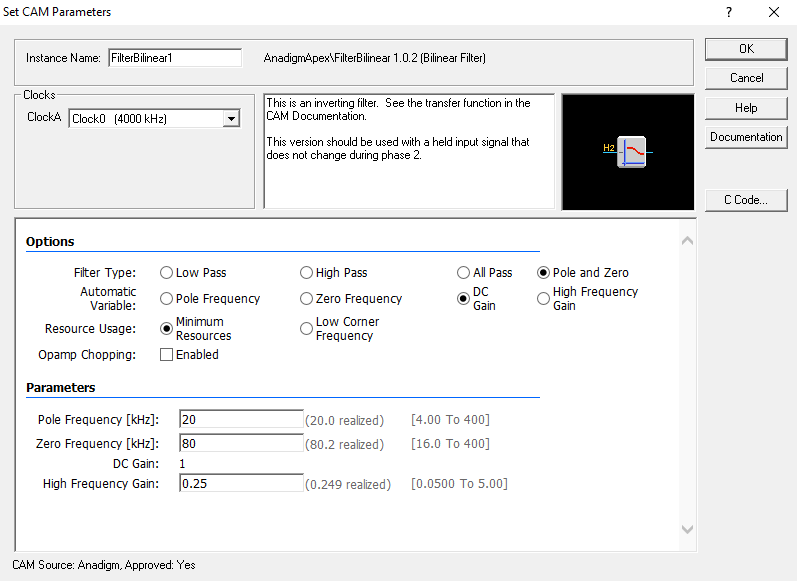
\includegraphics[width = 12cm]{G2_FilterBilinear_config.png}
\end{figure}

Los límites absolutos de los valores que se pueden ingresar para las frecuencias $f_{z}$ y $f_{p}$ son $[\frac{F_{c}}{1000}, \frac{F_{c}}{10}]$ donde $F_{c}$ es la frecuencia de reloj que se selecciona para el parámetro \textbf{ClockA} y los límites de ganancia están interrelacionados con los otros parámetros que pueden restringir el rango a menos que el límite absoluto el cual es $[0.01 \frac{\mathrm{V}}{\mathrm{V}}, 100.0\frac{\mathrm{V}}{\mathrm{V}}]$.  

\begin{table}[!hbp]                                      
\centering   
\caption{Valores para configurar un filtro bilineal como integrador de orden fraccionario en el rango de ordenes de 0.1 a 0.95.}                            
\label{tab:calculos_bilineal}                                        
\begin{tabular}{ccccc}                        
\hline                                              
$\bm{\alpha}$ & $\bm{f_{p}}\,\,$ [kHz] & $\bm{f_{z}}\,\,$ [kHz] & $\bm{G_{L}}$ & $\bm{G_{H}}$ \\            
\hline                                              
0.10 & 0.818182 & 1.222222 & 1.222222 & 0.818182 \\  
                                              
0.15 & 0.739130 & 1.352941 & 1.352941 & 0.739130 \\  
                                            
0.20 & 0.666667 & 1.500000 & 1.500000 & 0.666667 \\  
                                              
0.25 & 0.600000 & 1.666667 & 1.666667 & 0.600000 \\  
                                              
0.30 & 0.538462 & 1.857143 & 1.857143 & 0.538462 \\  
                                              
0.35 & 0.481481 & 2.076923 & 2.076923 & 0.481481 \\  
                                              
0.40 & 0.428571 & 2.333333 & 2.333333 & 0.428571 \\  
                                            
0.45 & 0.379310 & 2.636364 & 2.636364 & 0.379310 \\  
                                             
0.50 & 0.333333 & 3.000000 & 3.000000 & 0.333333 \\  
                                             
0.55 & 0.290323 & 3.444444 & 3.444444 & 0.290323 \\  
                                             
0.60 & 0.250000 & 4.000000 & 4.000000 & 0.250000 \\  
                                              
0.65 & 0.212121 & 4.714286 & 4.714286 & 0.212121 \\  
                                             
0.70 & 0.176471 & 5.666667 & 5.666667 & 0.176471 \\  
                                              
0.75 & 0.142857 & 7.000000 & 7.000000 & 0.142857 \\  
                                              
0.80 & 0.111111 & 9.000000 & 9.000000 & 0.111111 \\  
                                             
0.85 & 0.081081 & 12.333333 & 12.333333 & 0.081081 \\
                                              
0.90 & 0.052632 & 19.000000 & 19.000000 & 0.052632 \\
                                              
0.95 & 0.025641 & 39.000000 & 39.000000 & 0.025641 \\
\hline                                              
\end{tabular}                                                                
\end{table} 
  

Hay que tener presente que $F_{c}$ puede ser cualquier Clock, desde el 0 hasta el 5, en otras palabras, $F_{c}$ es igual a la ecuación (\ref{ec:clock_h}). Un análisis de todas las posibles frecuencias para $F_{c}$ dependiente de las subdivisiones dadas por $n$ se muestran en la Tabla \ref{tab:frecuencias_absolutas}, si se desea ver la tabla completa se puede usar el código del apéndice \ref{cod:A11_rango_de_frecuencias_absolutas_FilterBilinear}. 

\begin{table}[!hbp]                                      
\centering   
\caption{Rango de frecuencias absolutas dependiente de $F_{c}$ y el valor de $n$.}                            
\label{tab:frecuencias_absolutas}                                        
\begin{tabular}{cccc}                        
\hline                                              
$\bm{F_{c}}\,\,$ [kHz] & $\bm{n}$ & \textbf{min}$\bm{=F_{c} / 1000}\,\,$ [kHz] & \textbf{max}$\bm{=F_{c} /10}\,\,$ [kHz] \\                    
\hline                                              
16000.0000 & 1.0000 & 16.0000 & 1600.0000 \\
                                     
8000.0000 & 2.0000 & 8.0000 & 800.0000 \\   
                                     
4000.0000 & 4.0000 & 4.0000 & 400.0000 \\   

$\vdots$ & $\vdots$ & $\vdots$ & $\vdots$ \\  
 
31.6206 & 506.0000 & 0.0316 & 3.1621 \\     
                                    
31.4961 & 508.0000 & 0.0315 & 3.1496 \\     
                                    
31.3725 & 510.0000 & 0.0314 & 3.1373 \\      
\hline                                           
\end{tabular}                                                                
\end{table} 

Para demostrar que no todos los valores de la Tabla \ref{tab:calculos_bilineal} pueden ser implementados debido al rango de frecuencias absolutas mostradas en la Tabla \ref{tab:frecuencias_absolutas} consideremos los siguientes ejemplos:

Imaginemos que queremos implemetar un integrador de orden fraccionario con la aproximación de primer orden, un $\alpha = 0.9$ y escalado en frecuencia para que su ancho de banda se encuentre entre $100$ Hz y $10$ kHz. Dados los requerimientos anteriores $k_{f} = 2 \pi 1000$ y utilizando la Tabla \ref{tab:calculos_bilineal} sabemos que $f_{p} = 0.052632$, $f_{z} = 19.0$, $G_{L} = 19.0$ y $G_{H} = 0.052632$. Como se mencionó anteriormente la fuente de frecuencia de reloj principal $f_{c} = 16$ MHz no puede modificarse y de mismo modo se recomienda que Sys1 y Sys2 tampoco se modifiquen, es decir $m = 1$. Se opta por utilizar el Clock 0 para configurar el CAM FilterBilinear y que este dependa de Sys1 $=16$ MHz. Para que los datos que se ingresen en la ventana de configuración del CAM sean validos estos deben encontrase dentro del rango de frecuencias absolutas de la Tabla \ref{tab:frecuencias_absolutas}, por lo tanto se tiene que elegir un $n$ adecuado de tal manera que $F_{c}$ = Clock 0 = $\frac{\mathrm{Sys1}}{n}$ cumpla con los limites absolutos de frecuencia, en otras palabras que los parámetros $f_{z}$ y $f_{p}$ se encuentren dentro del rango $[\frac{F_{c}}{1000}, \frac{F_{c}}{10}]$. El rango de frecuencias en el que nos tenemos que encontrar para poder implemetentar el integrador es $[f_{p},f_{z}] = [0.052632, 19.0]$, no obstante el proceso de encontrar $n$ es muy laborioso debido a que podría haber más de un valor que haga posible que se encuentren dentro del rango, de mismo modo podría ocurrir el caso contrario y ninguna $n$ cumplir. Por esta razón en el Apéndice \ref{cod:A12_grafica_analisis_de_frecuencias_FilterBilinear} se muestra un código para resolver este problema, este genera una gráfica, ver Figura \ref{fig:T11_Analisis_de_frecuencias_FilterBilinear.eps}, la cual muestra la relación entre $n$ y el orden $\alpha$, en otras palabra hasta que orden fraccionario podemos implementar dependiendo del valor de $n$.

\begin{figure}[hbtp]
\caption{Análisis de orden fraccionario dependiente de $n$.} 
\label{fig:T11_Analisis_de_frecuencias_FilterBilinear.eps}
\centering
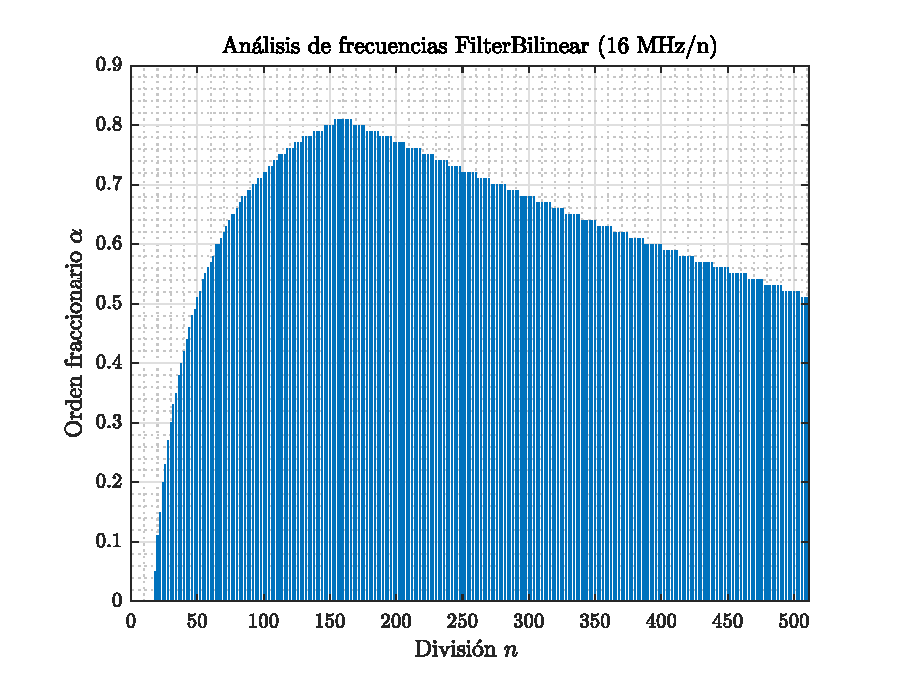
\includegraphics[width=12cm]{T11_Analisis_de_frecuencias_FilterBilinear.eps}
\end{figure}

Analizando la Figura \ref{fig:T11_Analisis_de_frecuencias_FilterBilinear.eps} podemos notar que $n = 160$ es el valor con el cual podemos implementar la mayor cantidad de integradores fraccionarios. Haciendo los cálculos Clock 0 = $\frac{16 \mathrm{MHz}}{160} = 100 \mathrm{kHz}$. No obstante únicamente podemos implementar integradores fracciones de orden $\alpha$ dentro del rango $[0.01, 0.81]$. En la Figura \ref{fig:G4_AD2_BilinearFilter_implementation.png} se muestra el diagrama de implementación en AnadigmDesigner2.

\begin{figure}[!ht] 
\caption{Implementación de integrador de orden fraccionario utilizando la aproximación de primer orden.}
\label{fig:G4_AD2_BilinearFilter_implementation.png}
\centering
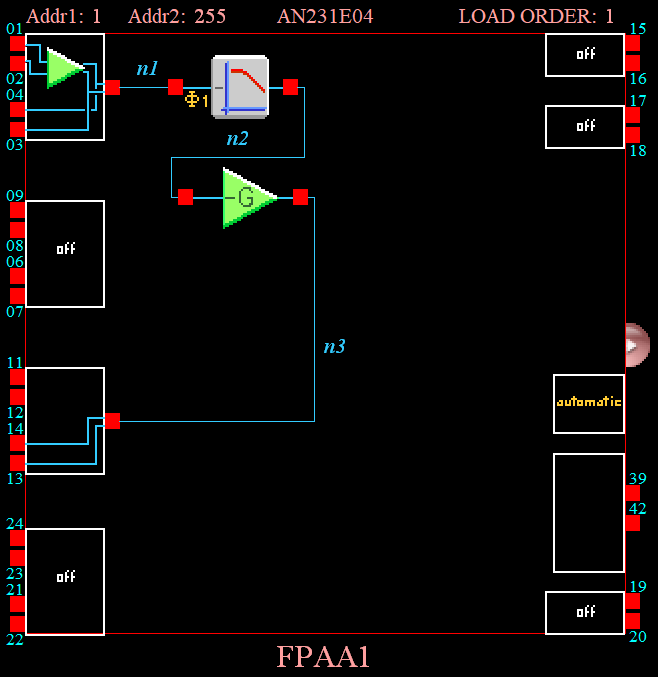
\includegraphics[width = 8cm]{G4_AD2_BilinearFilter_implementation.png}
\end{figure}

	\section{Implementación con aproximación de segundo}
	\chapter{Oscilador caótico utilizando integradores de orden fraccionario}

	\section{Oscilador caótico basado en funciones no lineales saturadas (SNLF)}
	
	Un oscilador caótico basado en funciones no lineales saturadas (SNLF) puede ser descrito por el siguiente sistema de ecuaciones diferenciales:

	\begin{equation} 
		\begin{array}{lcl}
		\dot{x} & = & y \\
		\dot{y} & = & z\\
		\dot{z} & = & -ax - by -cz + hf(x)
		\end{array}
		\label{ec:oscilador_SNLF}
	\end{equation}
	donde  $a, b, c$ y $h$ son coeficientes reales positivas positivos propuestos, con valores en el intervalo $[0, 1]$. $f(x)$ es una función lineal a trozos conocida como deestabilizadora o función saturada
	 
	 El sistema presenta un comportamiento dinámico no lineal gracias a la función saturada desestabilizante $f(x)$. El propósito de dicha función es retroalimentar al sistema y mantenerlo oscilando sin necesidad de una variable de entrada extra en el sistema. Además, esta función desestabilizante es la causante del comportamiento caótico del sistema. La SNLF puede ser descrita mediante una función PWL (PieceWise Linear) cuya forma dependerá del número de enrollamientos requeridos en el sistema caótico.
		
		\section{Función deestabilizadora}
	 El oscilador caótico basado en SNLF descrito en la ecuación (\ref{ec:oscilador_SNLF}) tiene su función saturación expresada como:
	 
	 \begin{equation}
		f(x) = \left\{ \begin{array}{lcl}
		k & \mathrm{si} & x > \beta \\
		sx & \mathrm{si} & - \beta \leq x \leq \beta  \\
		-k & \mathrm{si} & x < -\beta
		\end{array}
		\right.
		\label{ec:saturacion}
	\end{equation}
	donde el parámetro k representa la saturación del sistema, $\beta$ es el punto de quiebre en la función y $s$ es la pendiente entre tramos, en el apéndice \ref{cod:saturation_cust} se muestra una función de MATLAB que realiza esta función. 
	
	Estas funciones pueden generar $n$ cantidad de enrollamientos con la adecuada descripción matemática, en la Figura \ref{fig:Z1_saturacion} se muestra la representación gráfica de la función saturación. 
	
	\begin{figure}[!ht]
		\caption{Función no lineal saturada de dos enrollamientos.} 
		\label{fig:Z1_saturacion}
		\centering
		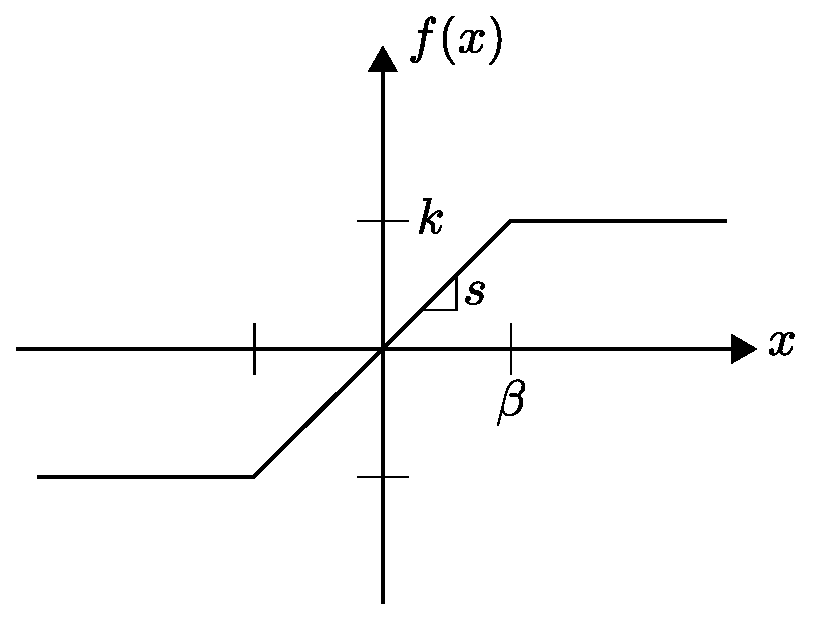
\includegraphics[width=8cm]{Z1_saturacion.eps}
	\end{figure}
	
		\section{Variables de estado del oscilador en orden fraccionario}
	 Para pasar el sistema de la ecuación (\ref{ec:oscilador_SNLF}) a orden fraccionario basta con modificarlo de la siguiente manera:
	 
	 \begin{equation}
		 \begin{array}{lcl}
		_{0}D_{t}^{\alpha}x & = & y \\
		_{0}D_{t}^{\alpha}y  & = & z\\
		_{0}D_{t}^{\alpha}z  & = & -ax - by -cz + hf(x)
		\end{array}
		\label{ec:frac_osc_imp}
	\end{equation}
	
	Las derivadas de orden entero en el sistema de ecuaciones diferenciales acopadas se reemplazan por derivadas de orden fraccionario. El sistema de la ecuación (\ref{ec:frac_osc_imp}) se puede solucionar utilizando el diagrama a bloques de la Figura \ref{fig:Z2_bloques}.
	
	\begin{figure}[!ht]
		\caption{Solución de sistema de orden fraccionario de la ecuación (\ref{ec:frac_osc_imp}).}
		\label{fig:Z2_bloques}
		\centering
		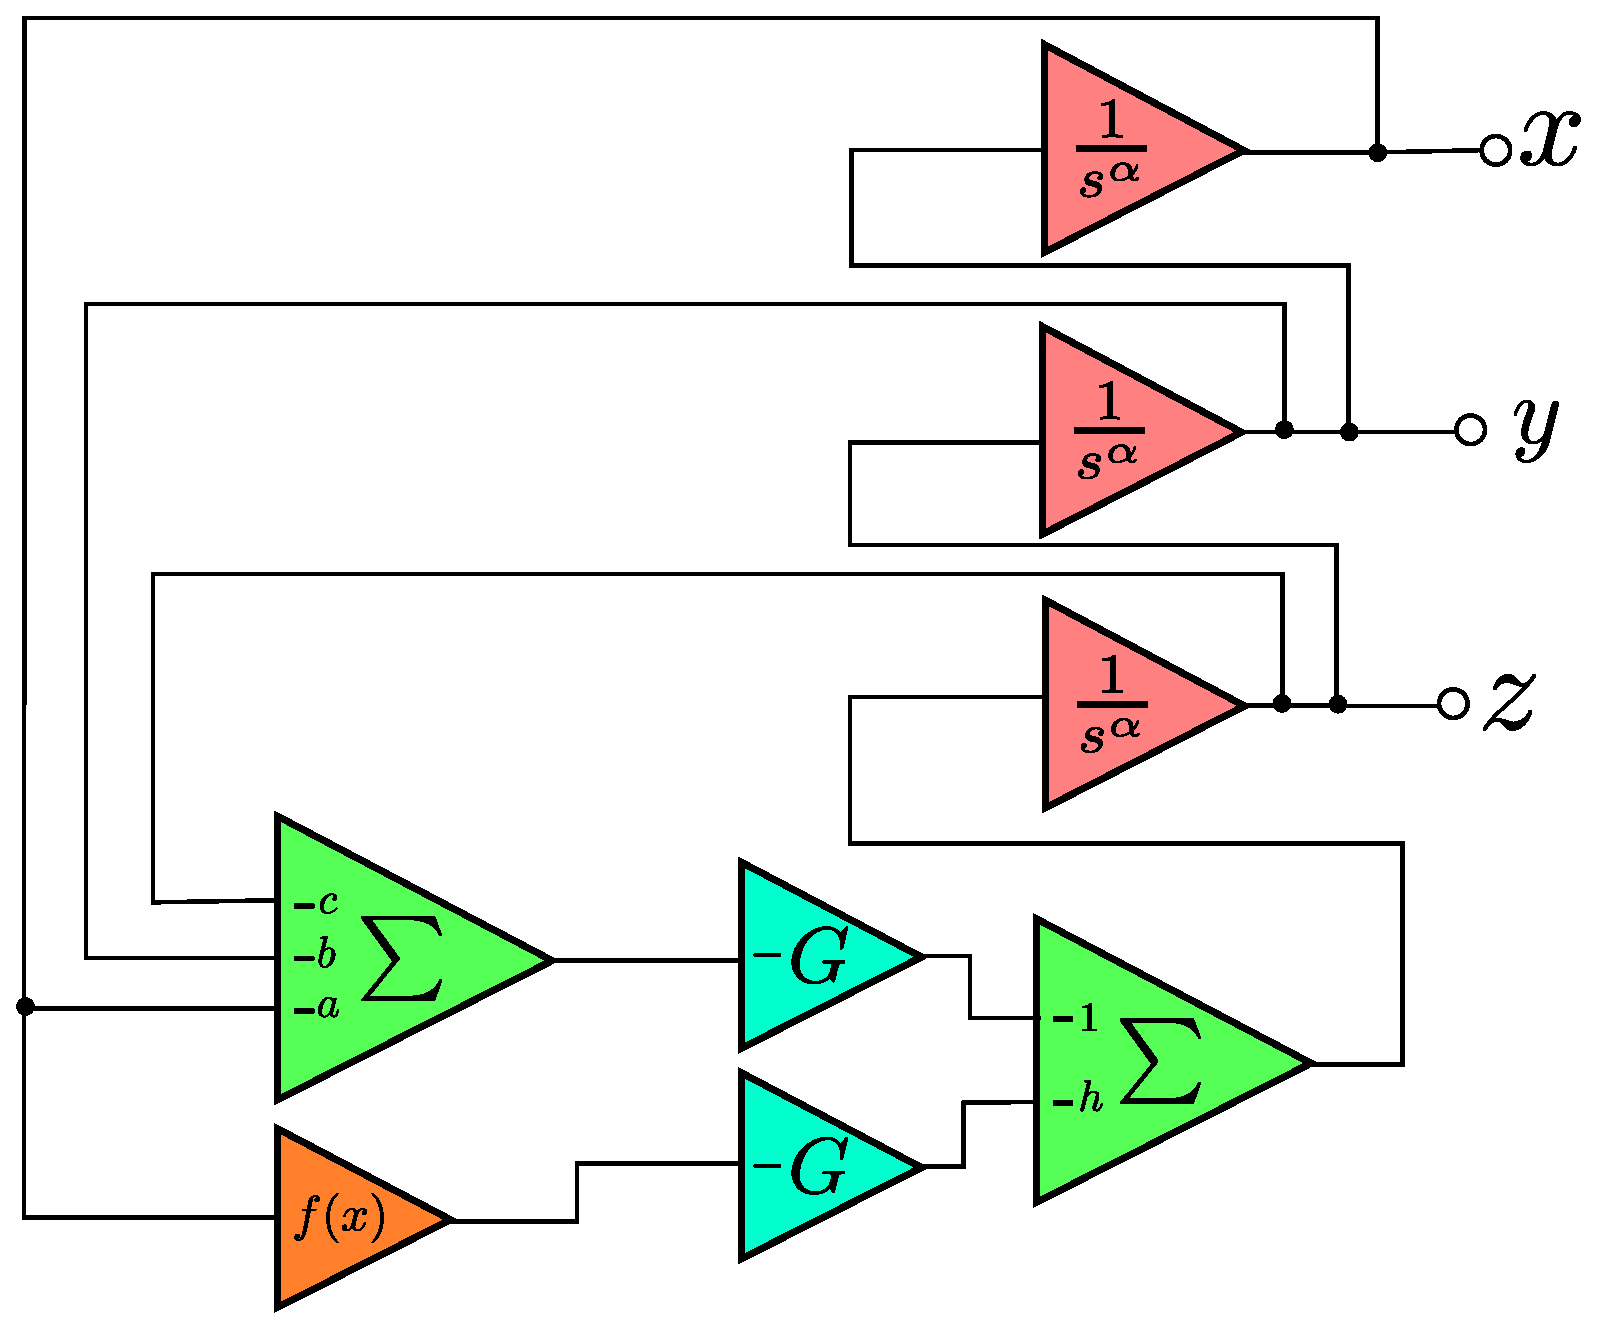
\includegraphics[width=8cm]{Z2_bloques.eps}
	\end{figure}
	
	\section{Implementación en FPAA}
	
	La implementación del oscilador caótico (SNLF) con integradores de orden fraccionario requirió de los 4 FPAA (es necesario colocar los jumpers J8, J9, J10 y ACT1,2,3,4) con los que cuenta la tarjeta. Se optimizó de manera que utilizara la menor cantidad de conexiones externas y se distribuyeron los CAM de modo que fuera sencillo modificar los integradores fraccionarios entre sus distintas aproximaciones o dicho de manera más precisa, entre  sus distintas topologías. 
	
	Para poder realizar las mediciones físicas es necesario utilizar los filtros Rauch que se mencionaron en la sección \ref{sec:rauch} (activar los DIP switches S13 y S12), esto debido a la necesidad de convertir la señal diferencial con que trabaja la FPAA por una single-ended. De mismo modo para interconectar las FPAA es necesario realizar las conexiones físicas sobre la tarjeta, esto se logra activando diversos DIP switches según convenga, en la Tabla \ref{tab:resumen_de_imp} se resumen las conexiones físicas que se tienen que realizar sobre la tarjeta. 
	
	\begin{table}[!ht]                                      
		\centering   
		\caption{Conexiones de DIP switches, jumpers y cables externos.}                            
		\label{tab:resumen_de_imp}                                       
			\begin{tabular}{c c c}                        
			\hline                                              
			Switch & Jumper & Cables externos\\            
			\hline       
			{\color{magenta} S$3$ $\quad2\downarrow$}& J8 & FPAA1 O3 $\rightarrow$ FPAA3 I5\\  
			{\color{magenta} S$5$ $\quad2\downarrow$}& J9& FPAA1 I5 $\rightarrow$ FPAA3 O5\\
			{\color{red} S$4$ $\quad2\uparrow$}&J10&\\ 
			{\color{red} S$6$ $\quad2\uparrow$}&ACT1 &\\
			{\color{blue} S$7$ $\quad2\uparrow$}& ACT2 &\\ 
			S12& ACT3 &\\ 
			S13& ACT4 &\\ 
			\hline                                 
			\end{tabular}                                                             
	\end{table}	
	
	\subsection{Configuración bilineal polo y cero}
	En la Figura \ref{fig:Y1_implementacion} se presenta el diseño final del oscilador caótico (SNLF) implementado en la tarjeta utilizando la configuración bilineal polo y cero con un  orden $\alpha = 0.8$ y con las constantes $a =4$, $b = 0.7$, $c = 0.7$ y $h = 4$. La función de saturación se propuso con los parámetros $k = 2$, $s = 1$ y $\beta= 1.5$ dando como resultado el comportamiento mostrado en la Figura \ref{fig:Z8_saturacion}. Es necesario generar la lookup table utilizando los códigos de los apéndices \ref{cod:saturation_cust} y \ref{cod:D1_Look_up_table}.
	
	\begin{figure}[!ht]
		\caption{Diagrama de implementación en AD2 configuración bilineal polo y cero.} 
		\label{fig:Y1_implementacion}
		\centering
		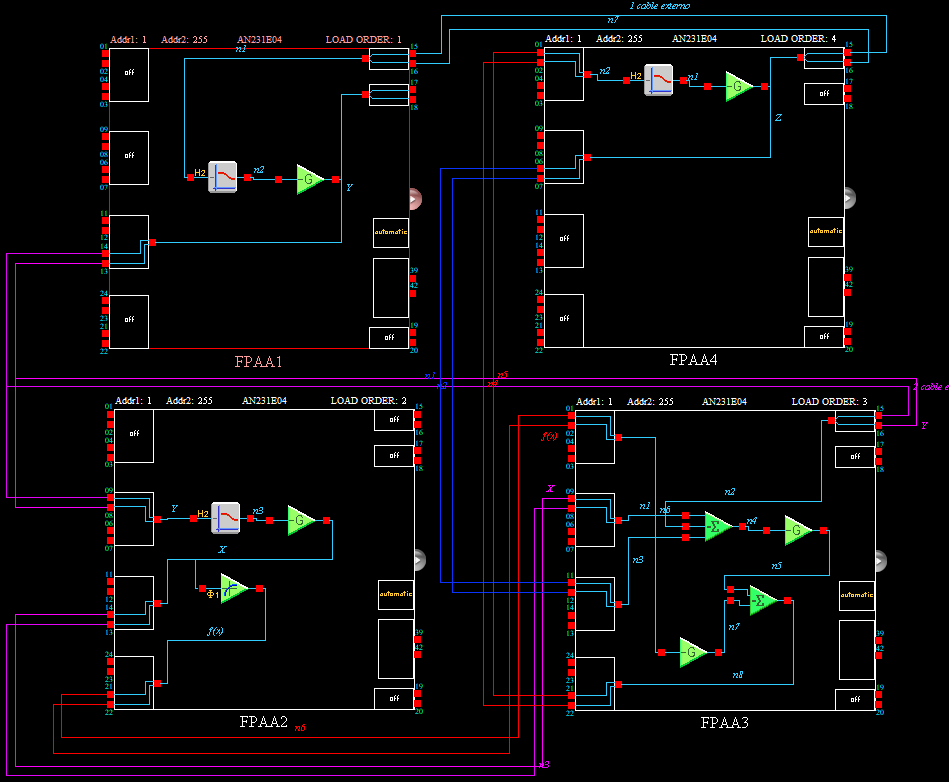
\includegraphics[width=14cm]{Y1_implementacion.png}
	\end{figure}
	
	Los 4 FPAA se configuraron con las mismas frecuencias de reloj las cuales se muestran en la Figura \ref{fig:Z3_relojes}. Hay que recordar que para $\alpha = 0.8$ los valores para el integrador con aproximación bilineal polo y cero son los siguientes:
	
	\begin{table}[!hbp]                                      
		\centering   
		\caption{Valores para configurar un filtro bilineal como integrador de orden fraccionario con $\alpha = 0.8$.}                            
		\label{tab:respaso}                                        
			\begin{tabular}{ccccc}                        
			\hline                                              
			$\bm{\alpha}$ & $\bm{f_{p}}\,\,$ [kHz] & $\bm{f_{z}}\,\,$ [kHz] & $\bm{G_{L}}$ & $\bm{G_{H}}$ \\            
			\hline                                                                                       
			0.80 & 0.111111 & 9.000000 & 9.000000 & 0.111111 \\  
			\hline                                              
			\end{tabular}                                                                
	\end{table} 
	\begin{figure}[!ht] 
		\caption{Configuración de clocks de todos los FPAA.}
		\label{fig:Z3_relojes}
		\centering
		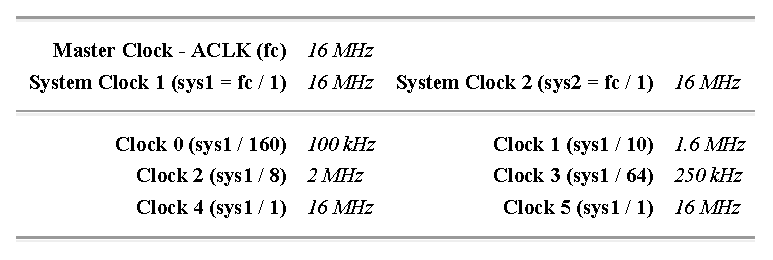
\includegraphics[width = 12cm]{Z3_relojes.eps}
	\end{figure}
	
	En las Figuras \ref{fig:Z4_FPAA1}, \ref{fig:Z5_FPAA2}, \ref{fig:Z6_FPAA3}, \ref{fig:Z7_FPAA4} se muestran las configuraciones de los CAM desde la FPAA1 hasta la 4.
	\begin{figure}[!ht] 
		\caption{Configuración de los CAM de FPAA1.}
		\label{fig:Z4_FPAA1}
		\centering
		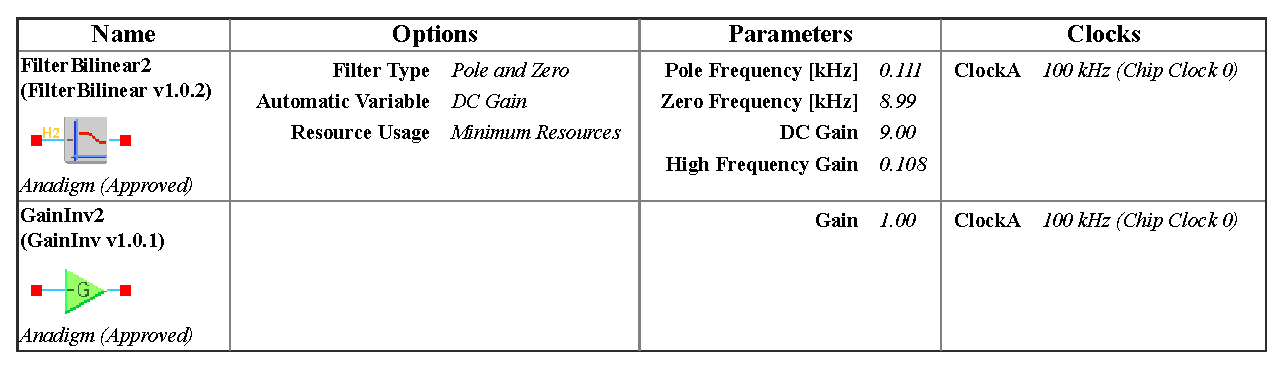
\includegraphics[width = 14cm]{Z4_FPAA1.eps}
	\end{figure}
	
	\begin{figure}[!ht] 
		\caption{Configuración de los CAM de FPAA2.}
		\label{fig:Z5_FPAA2}
		\centering
		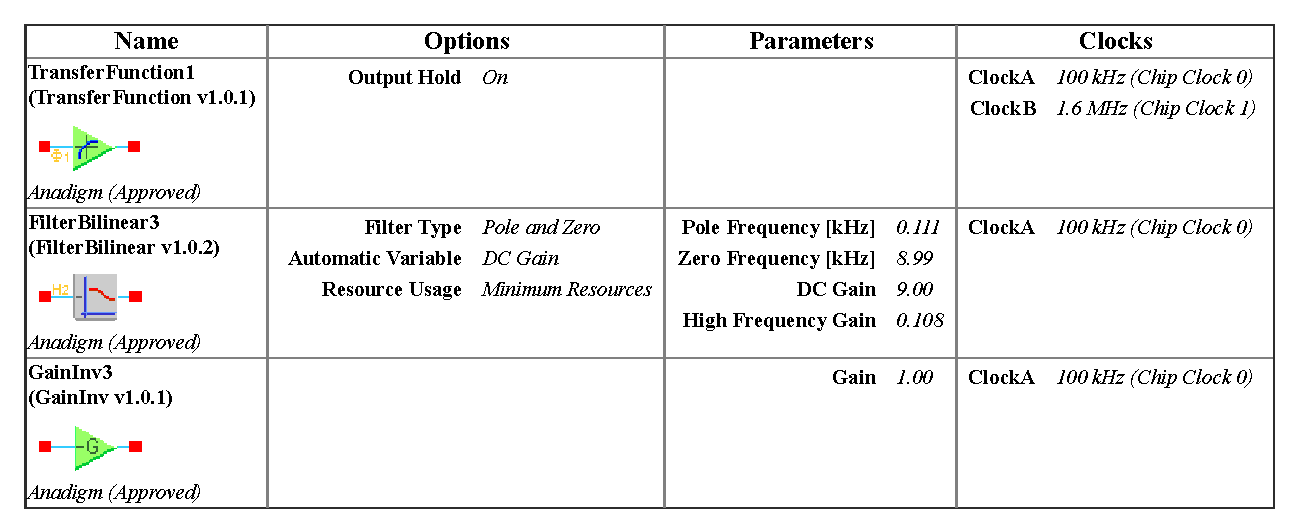
\includegraphics[width = 14cm]{Z5_FPAA2.eps}
	\end{figure}
	
	El comportamiento del oscilador depende directamente de los valores de los parámetros que se eligieron, la función de saturación y el orden fraccionario. Si se modifica ligeramente la función de saturación el sistema pierde su capacidad de oscilar, lo mismo ocurre si se modifica alguno de los parámetros del sistema. 
	
	En las Figuras \ref{fig:fase_imp_osc} y \ref{fig:temporal_imp} se muestran los resultados experimentales. En la primera se muestran los planos de fase o atractores  del sistema y en la segunda la respuesta en el dominio temporal de cada una de estas.
	\begin{figure}[!ht] 
		\caption{Configuración de los CAM de FPAA3.}
		\label{fig:Z6_FPAA3}
		\centering
		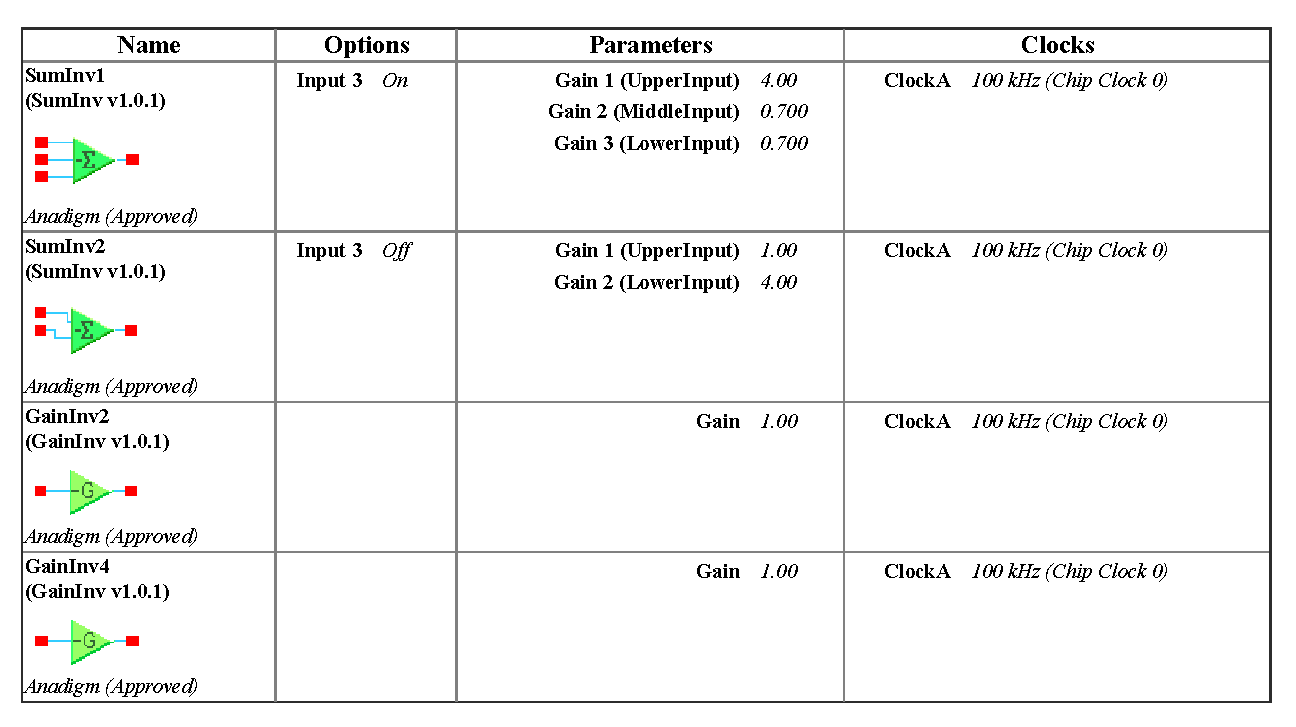
\includegraphics[width = 14cm]{Z6_FPAA3.eps}
	\end{figure}
	
	\begin{figure}[!ht] 
		\caption{Configuración de los CAM de FPAA4.}
		\label{fig:Z7_FPAA4}
		\centering
		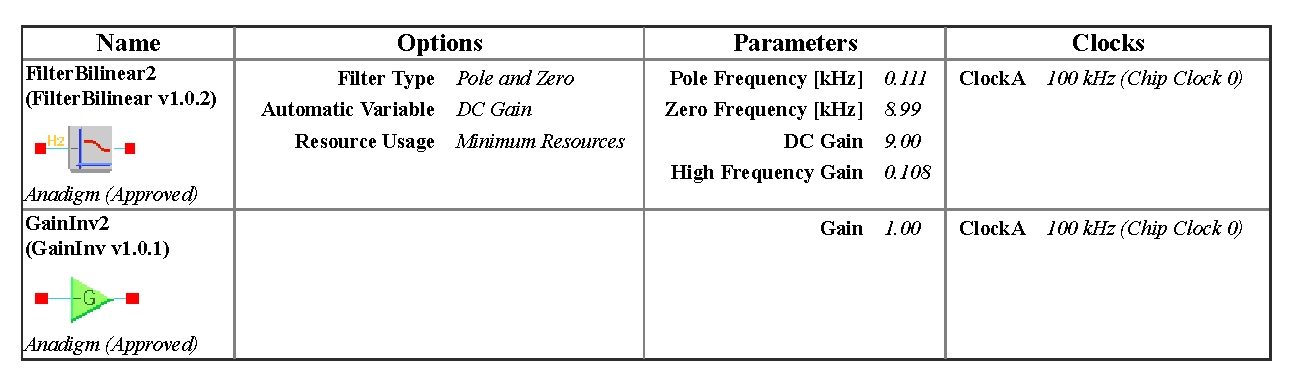
\includegraphics[width = 14cm]{Z7_FPAA4.eps}
	\end{figure}
	
	\begin{figure}[!ht]
		\caption{Función de saturación $k = 2$, $s = 1$ y $\beta= 1.5$.} 
		\label{fig:Z8_saturacion}
		\centering
		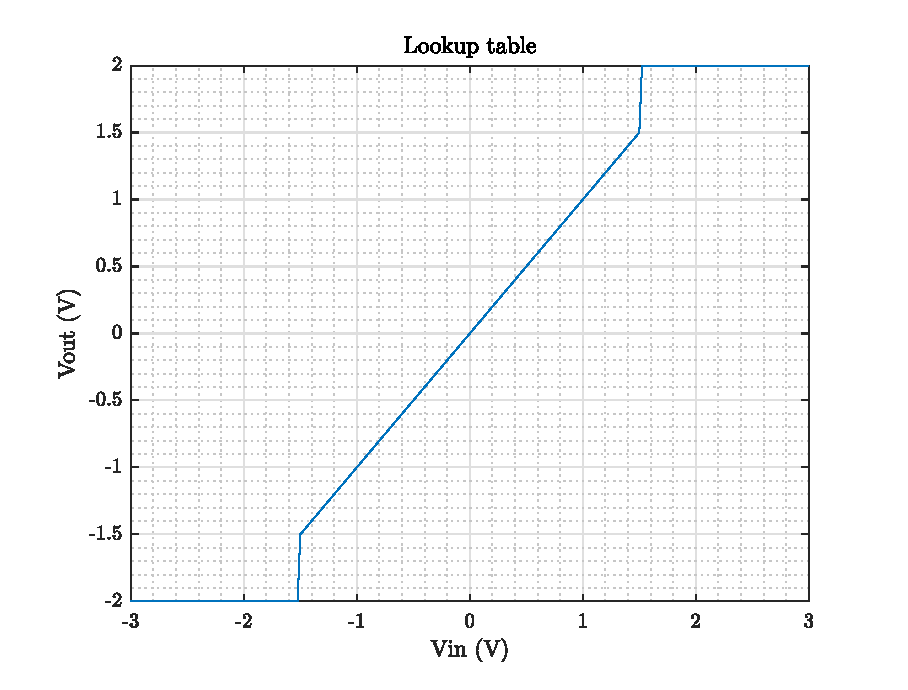
\includegraphics[width=10cm]{Z8_saturacion.eps}
	\end{figure}

	
	\begin{figure}[!ht]
	\caption{Vistas de plano fase del comportamiento del oscilador caótico con $\alpha = 0.8$ y dos enrollamientos.}
	\label{fig:fase_imp_osc}
	  \begin{subfigure}[b]{0.3\textwidth}
	    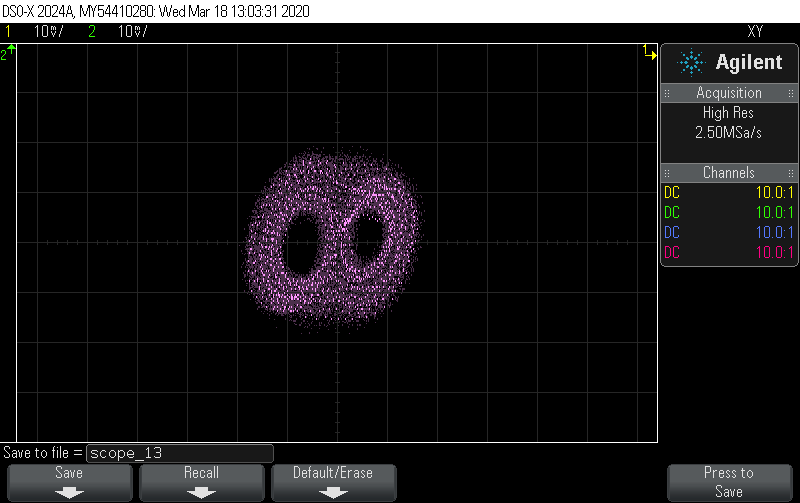
\includegraphics[trim={6cm 2cm 9cm 2cm},clip,width=\textwidth]{Y2_X_vs_Y.png}
	    \caption{$x$ vs $y$}
	    \label{Y2_X_vs_Y}
	  \end{subfigure}
	  \hfill
	  \begin{subfigure}[b]{0.3\textwidth}
	    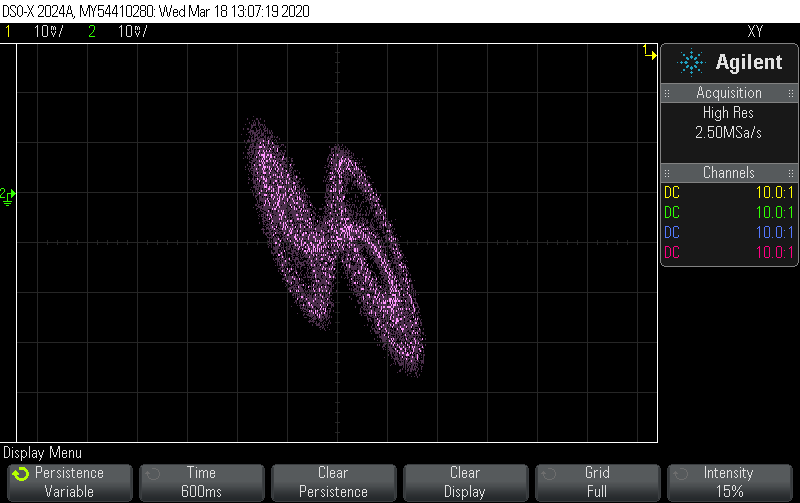
\includegraphics[trim={6cm 2cm 9cm 2cm},clip,width=\textwidth]{Y4_X_vs_Z.png}
	    \caption{$x$ vs $z$}
	    \label{fig:Y4_X_vs_Z}
	  \end{subfigure}
	  \hfill
	  \begin{subfigure}[b]{0.3\textwidth}
	    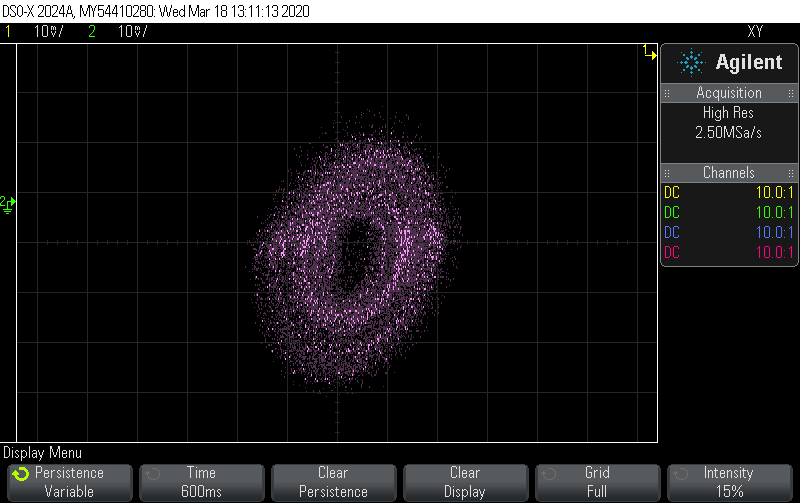
\includegraphics[trim={6cm 2cm 9cm 2cm},clip,width=\textwidth]{Y6_Y_vs_Z.png}
	    \caption{$y$ vs $z$}
	    \label{Y6_Y_vs_Z}
	  \end{subfigure}
	\end{figure}
	
	\begin{figure}[!ht]
	\caption{Respuesta en el dominio temporal de oscilador caótico con $\alpha = 0.8$ y dos enrollamientos.}
	\label{fig:temporal_imp}
	  \begin{subfigure}[b]{0.3\textwidth}
	    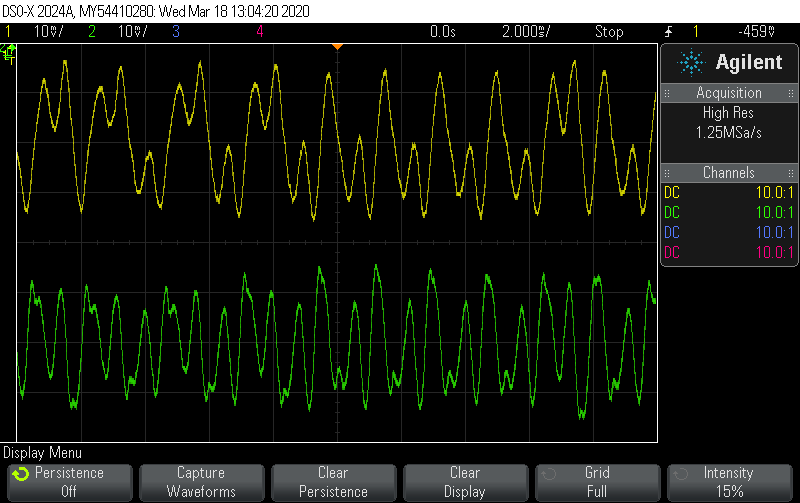
\includegraphics[trim={6cm 2cm 9cm 2cm},clip,width=\textwidth]{Y3_X_vs_Y_signal.png}
	    \caption{$x$ vs $y$}
	    \label{fig:Y3_X_vs_Y_signal}
	  \end{subfigure}
	  \hfill
	  \begin{subfigure}[b]{0.3\textwidth}
	    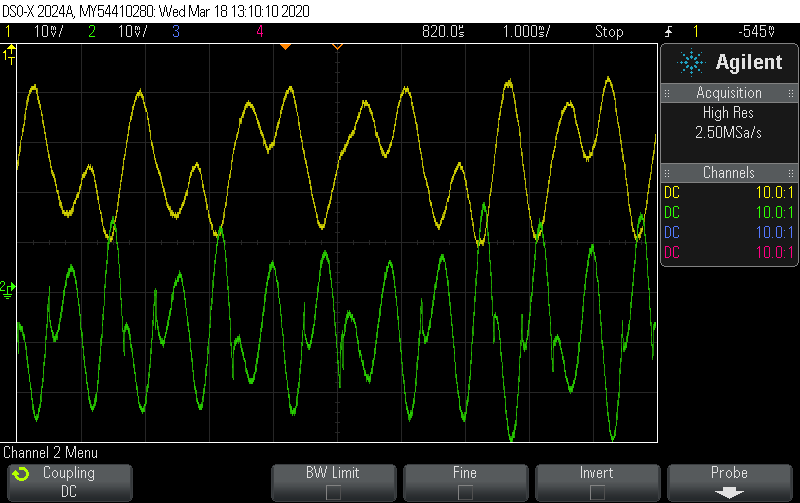
\includegraphics[trim={6cm 2cm 9cm 2cm},clip,width=\textwidth]{Y5_X_vs_Z_signal.png}
	    \caption{$x$ vs $z$}
	    \label{fig:Y5_X_vs_Z_signal}
	  \end{subfigure}
	  \hfill
	  \begin{subfigure}[b]{0.3\textwidth}
	    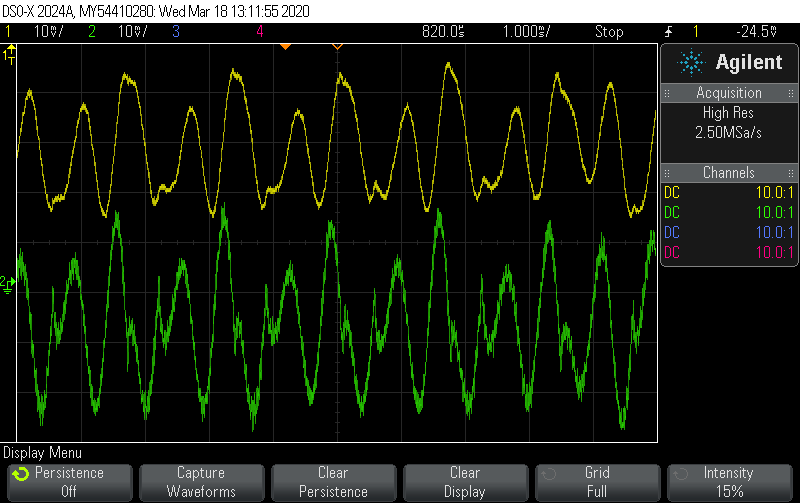
\includegraphics[trim={6cm 2cm 9cm 2cm},clip,width=\textwidth]{Y7_Y_vs_Z_signal.png}
	    \caption{$y$ vs $z$}
	    \label{fig:Y7_Y_vs_Z_signal}
	  \end{subfigure}
	\end{figure}
	
	\subsection{Configuración bilineal suma de filtros}
	
	En la Figura \ref{fig:Y1p_implementacion} se presenta el diseño final del oscilador caótico (SNLF) implementado en la tarjeta utilizando la configuración bilineal suma de filtros con un  orden $\alpha = 0.9$ y con las constantes $a =4$, $b = 0.7$, $c = 0.7$ y $h = 4$. 
	
	\begin{figure}[!ht]
		\caption{Diagrama de implementación en AD2 configuración bilineal suma de filtros.} 
		\label{fig:Y1p_implementacion}
		\centering
		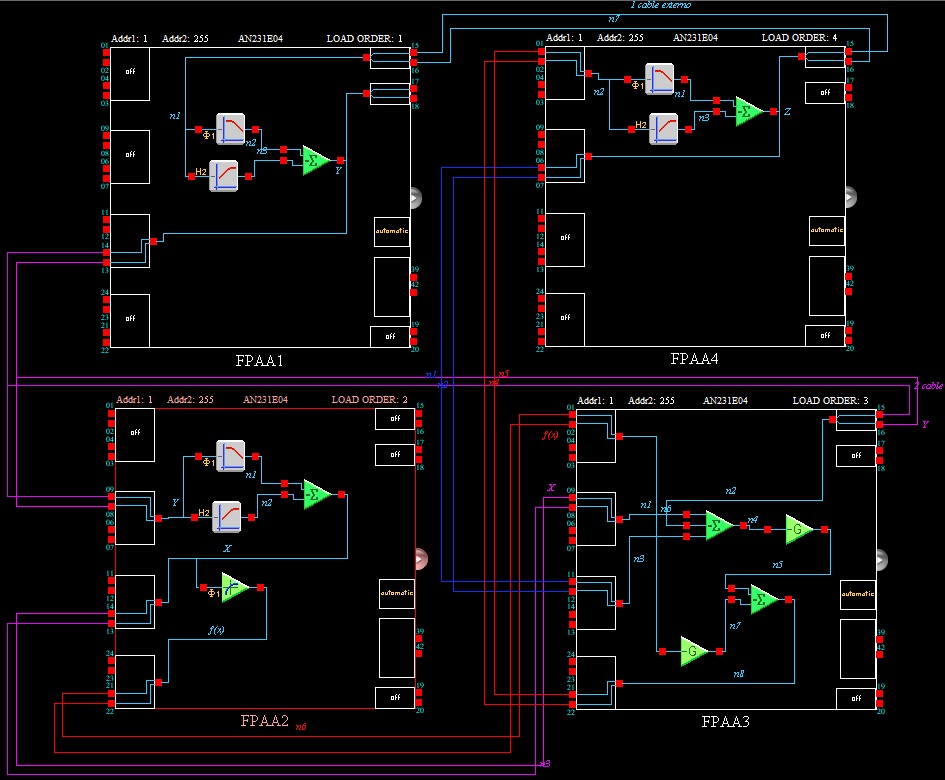
\includegraphics[width=14cm]{Y1p_implementacion.png}
	\end{figure}
	
	Los 4 FPAA se configuraron con las mismas frecuencias de reloj las cuales se muestran en la Figura \ref{fig:Z3p_relojes}. Hay que recordar que para $\alpha = 0.9$ los valores para el integrador con aproximación bilineal suma de filtros son los siguientes:
	
	\begin{table}[!hbp]                                      
		\centering   
		\caption{Valores para configurar implementación suma de pasabajas y paaltas de ordenes de 0.1 a 0.95.}                            
		\label{tab:repaso2}                                        
			\begin{tabular}{cccc}                        
			\hline                                              
			$\bm{\alpha}$ & $\bm{G_{1}}\,\,$ [LP] & $\bm{G_{2}}\,\,$ [HP] & $\bm{f_{0}}\,\,$ [kHz]  \\            
			\hline                                                                         
			0.90 & 19.000000 & 0.052632 & 0.052632 \\
			\hline                                              
			\end{tabular}                                                                
	\end{table} 	
	
	
	\begin{figure}[!ht] 
		\caption{Configuración de clocks de todos los FPAA.}
		\label{fig:Z3p_relojes}
		\centering
		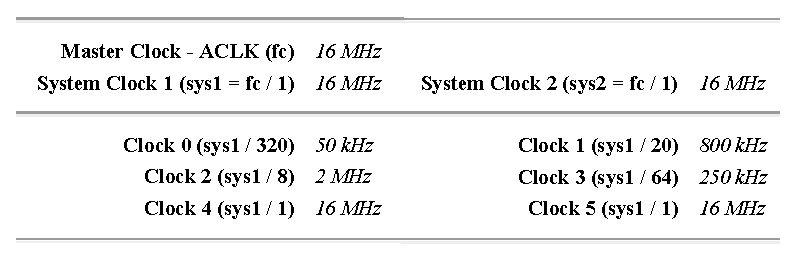
\includegraphics[width = 12cm]{Z3p_relojes.eps}
	\end{figure}
	
	En las Figuras \ref{fig:Z4p_FPAA1}, \ref{fig:Z5p_FPAA2}, \ref{fig:Z6p_FPAA3}, \ref{fig:Z7p_FPAA4} se muestran las configuraciones de los CAM desde la FPAA1 hasta la 4.
	\begin{figure}[!ht] 
		\caption{Configuración de los CAM de FPAA1.}
		\label{fig:Z4p_FPAA1}
		\centering
		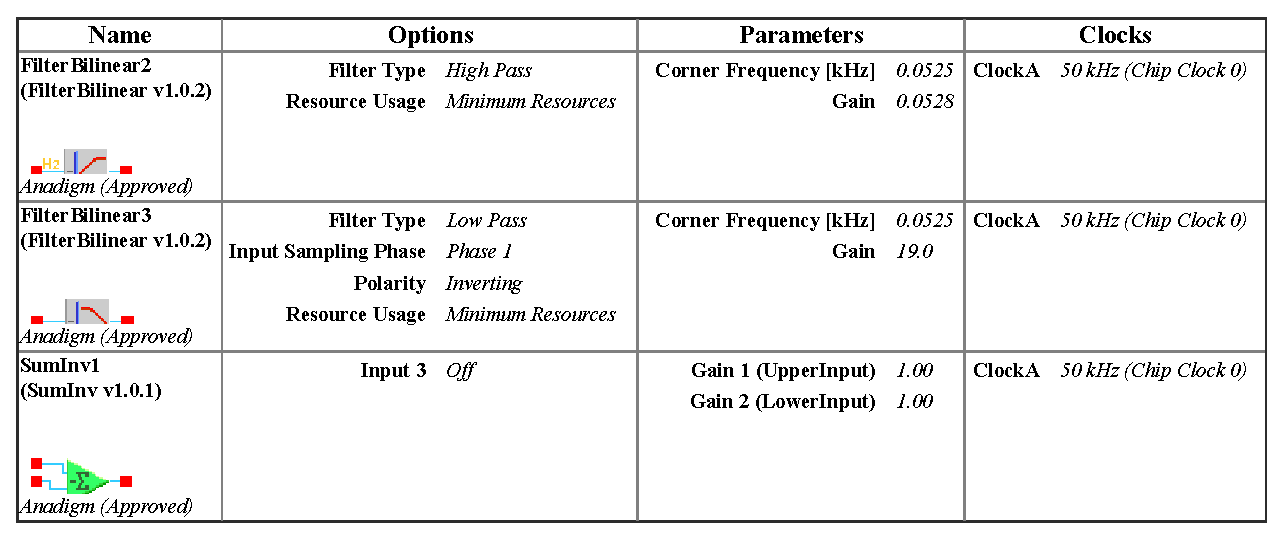
\includegraphics[width = 14cm]{Z4p_FPAA1.eps}
	\end{figure}
	
	\begin{figure}[!ht] 
		\caption{Configuración de los CAM de FPAA2.}
		\label{fig:Z5p_FPAA2}
		\centering
		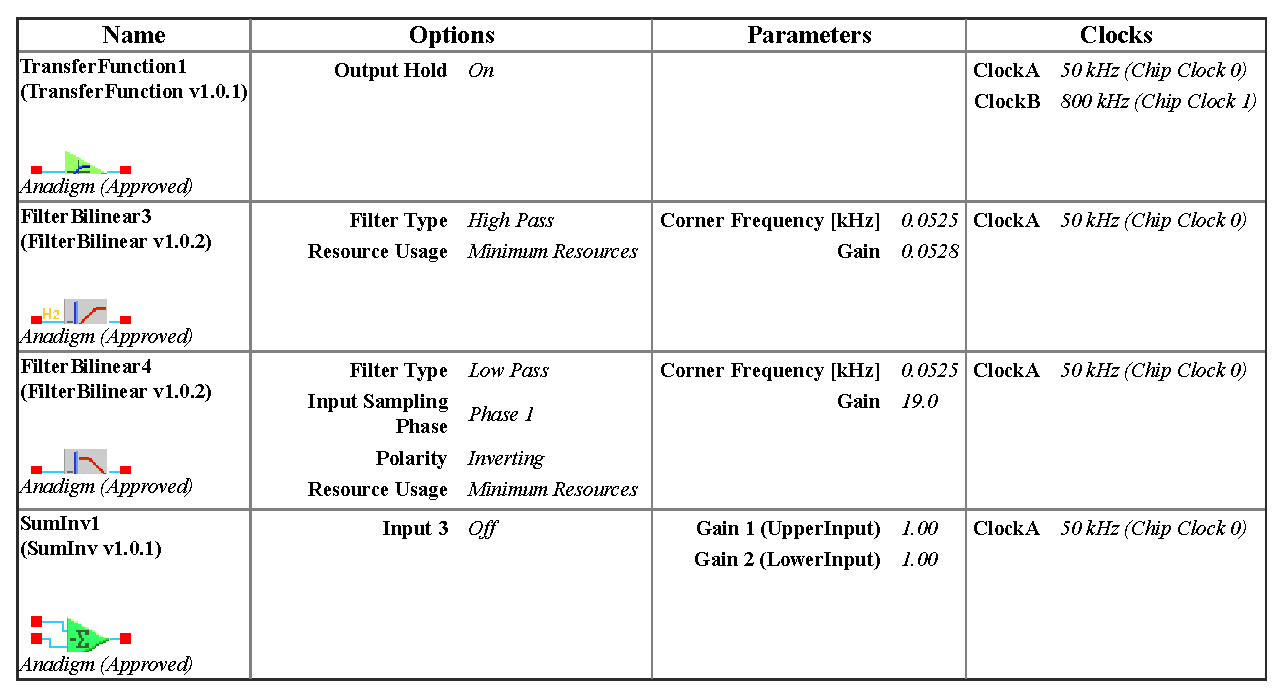
\includegraphics[width = 14cm]{Z5p_FPAA2.eps}
	\end{figure}
	
	En las Figuras \ref{fig:fasep_imp_osc} y \ref{fig:temporalp_imp} se muestran los resultados experimentales. En la primera se muestran los planos de fase o atractores  del sistema y en la segunda la respuesta en el dominio temporal de cada una de estas.
	\begin{figure}[!ht] 
		\caption{Configuración de los CAM de FPAA3.}
		\label{fig:Z6p_FPAA3}
		\centering
		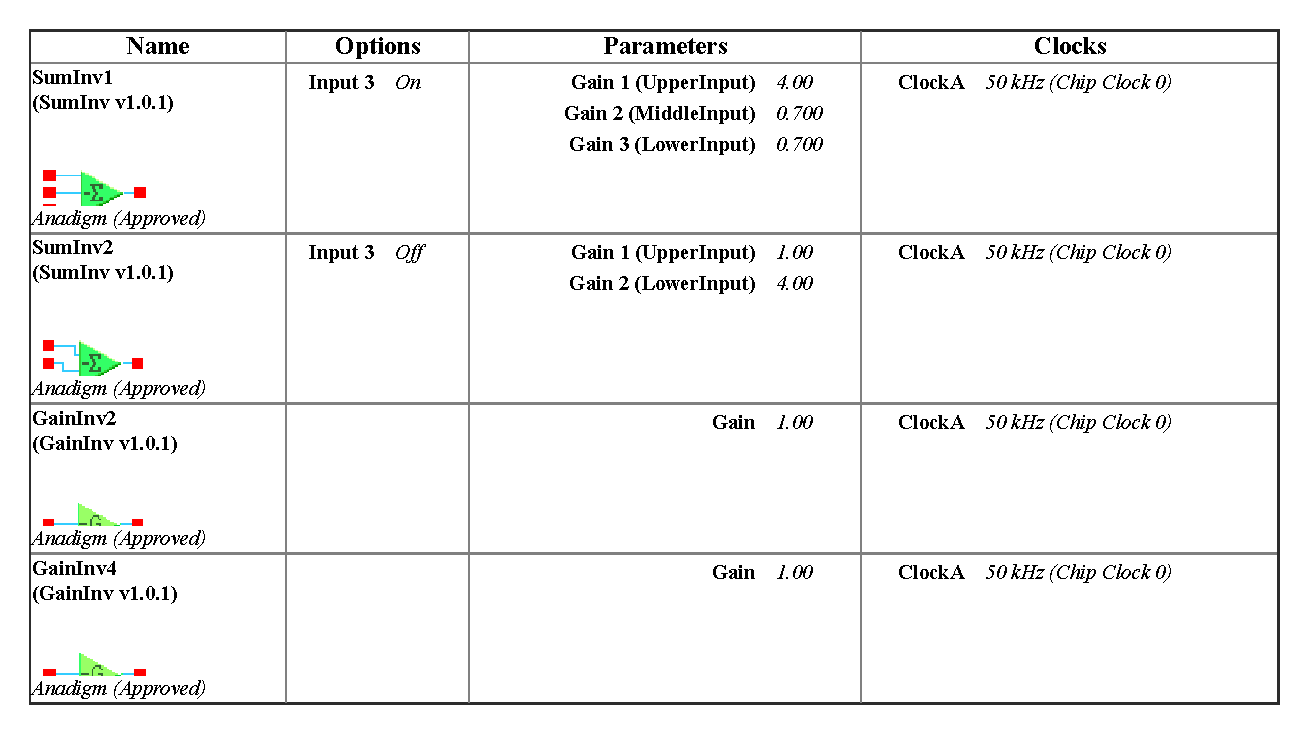
\includegraphics[width = 14cm]{Z6p_FPAA3.eps}
	\end{figure}
	
	\begin{figure}[!ht] 
		\caption{Configuración de los CAM de FPAA4.}
		\label{fig:Z7p_FPAA4}
		\centering
		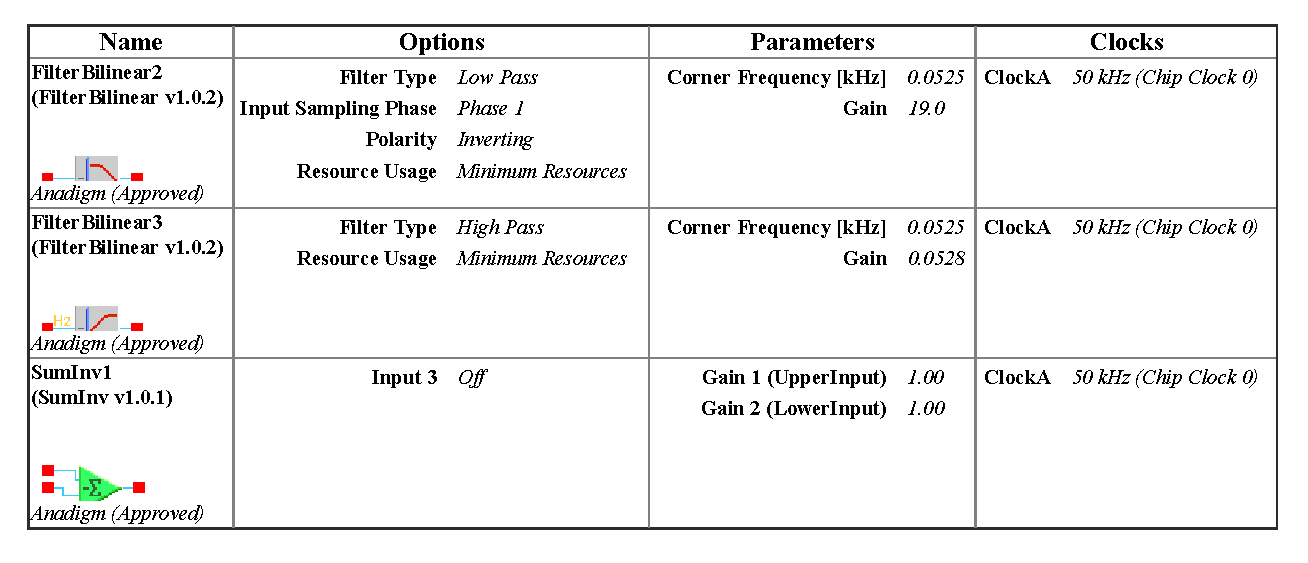
\includegraphics[width = 14cm]{Z7p_FPAA4.eps}
	\end{figure}
	

	
	\begin{figure}[!ht]
	\caption{Vistas de plano fase del comportamiento del oscilador caótico con $\alpha = 0.8$ y dos enrollamientos.}
	\label{fig:fasep_imp_osc}
	  \begin{subfigure}[b]{0.3\textwidth}
	    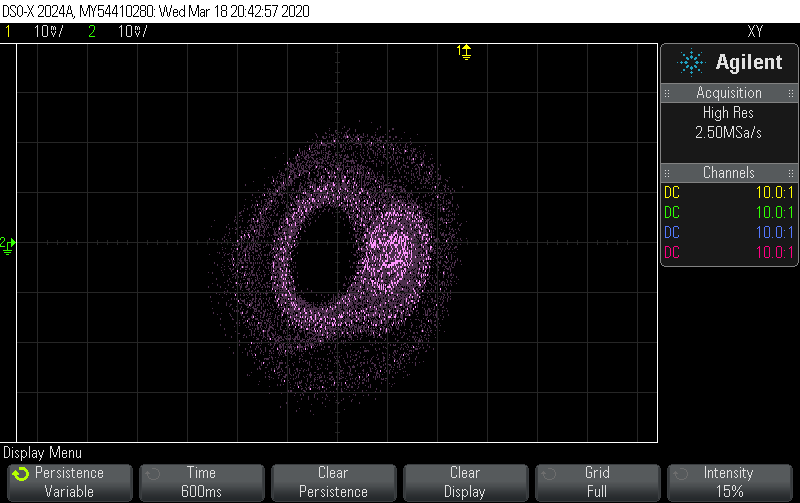
\includegraphics[trim={6cm 2cm 9cm 2cm},clip,width=\textwidth]{Y2p_X_vs_Y.png}
	    \caption{$x$ vs $y$}
	    \label{Y2p_X_vs_Y}
	  \end{subfigure}
	  \hfill
	  \begin{subfigure}[b]{0.3\textwidth}
	    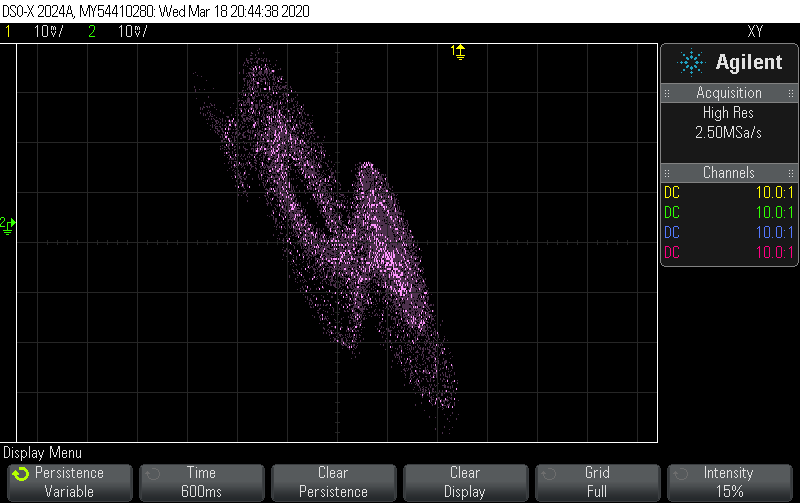
\includegraphics[trim={6cm 2cm 9cm 2cm},clip,width=\textwidth]{Y4p_X_vs_Z.png}
	    \caption{$x$ vs $z$}
	    \label{fig:Yp4_X_vs_Z}
	  \end{subfigure}
	  \hfill
	  \begin{subfigure}[b]{0.3\textwidth}
	    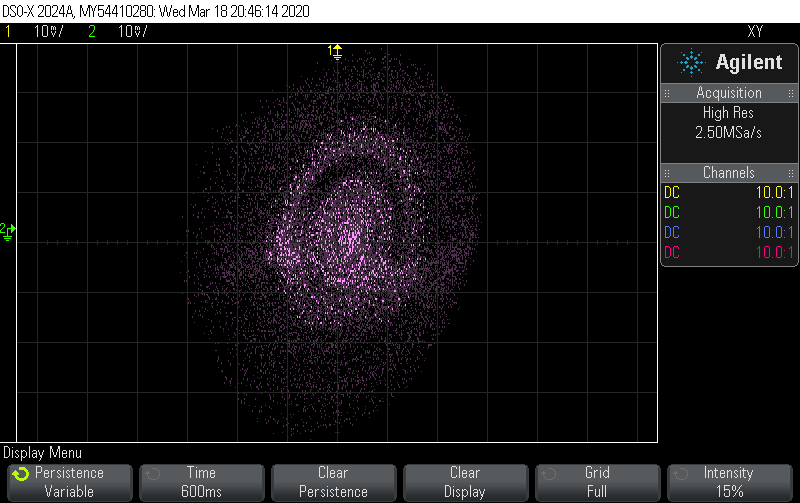
\includegraphics[trim={6cm 2cm 9cm 2cm},clip,width=\textwidth]{Y6p_Y_vs_Z.png}
	    \caption{$y$ vs $z$}
	    \label{Y6p_Y_vs_Z}
	  \end{subfigure}
	\end{figure}
	
	\begin{figure}[!ht]
	\caption{Respuesta en el dominio temporal de oscilador caótico con $\alpha = 0.8$ y dos enrollamientos.}
	\label{fig:temporalp_imp}
	  \begin{subfigure}[b]{0.3\textwidth}
	    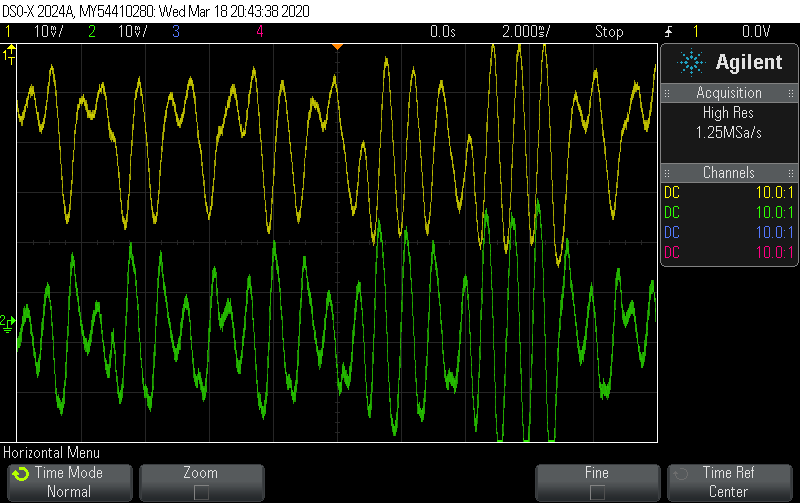
\includegraphics[trim={6cm 2cm 9cm 2cm},clip,width=\textwidth]{Y3p_X_vs_Y_signal.png}
	    \caption{$x$ vs $y$}
	    \label{fig:Y3p_X_vs_Y_signal}
	  \end{subfigure}
	  \hfill
	  \begin{subfigure}[b]{0.3\textwidth}
	    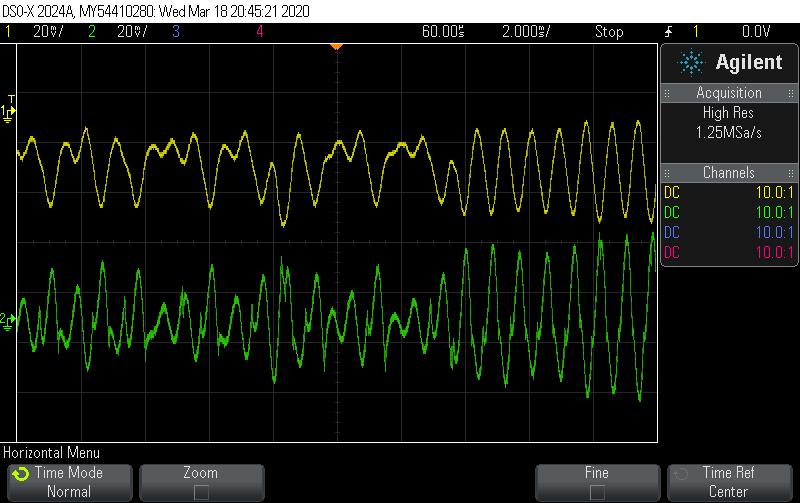
\includegraphics[trim={6cm 2cm 9cm 2cm},clip,width=\textwidth]{Y5p_X_vs_Z_signal.png}
	    \caption{$x$ vs $z$}
	    \label{fig:Y5p_X_vs_Z_signal}
	  \end{subfigure}
	  \hfill
	  \begin{subfigure}[b]{0.3\textwidth}
	    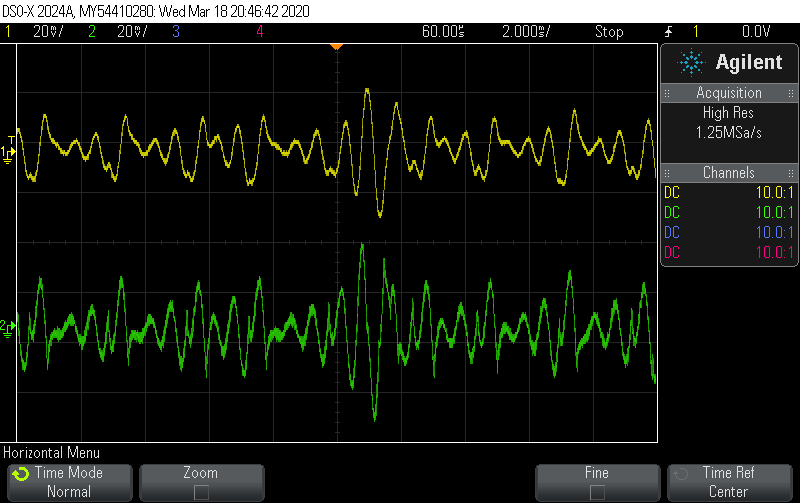
\includegraphics[trim={6cm 2cm 9cm 2cm},clip,width=\textwidth]{Y7p_Y_vs_Z_signal.png}
	    \caption{$y$ vs $z$}
	    \label{fig:Y7p_Y_vs_Z_signal}
	  \end{subfigure}
	\end{figure}

\appendix
	\chapter{Códigos}

\lstinputlisting[style = MATLAB, caption =  Función syms2tf, label = cod:syms2tf]{codigos/syms2tf.m}

\lstinputlisting[style = MATLAB, caption =  Función cfetf, label = cod:cfetf]{codigos/cfetf.m}

\lstinputlisting[style = MATLAB, caption = Simulación spice pasabajas.cir, label = cod:LTspice_simulacion]{LTspice_simulacion/pasabajas.cir}

\lstinputlisting[style = MATLAB, caption = Diagramas de Bode comparativos ideal vs spice vs experimental, label = cod:diagramas_bode_comparativos]{codigos/Analisis_Bode_ELVIS/diagramas_bode_comparativos.m}

\lstinputlisting[style = MATLAB, caption =  A10\_{}calculo\_{}valores\_{}FilterBilinear, label = cod:A10_calculo_valores_FilterBilienar]{codigos/A10_calculo_valores_FilterBilinear.m}

\lstinputlisting[style = MATLAB, caption =  A11\_{}rango\_{}de\_{}frecuencias\_{}absolutas\_{}FilterBilinear, label = cod:A11_rango_de_frecuencias_absolutas_FilterBilinear]{codigos/A11_rango_de_frecuencias_absolutas_FilterBilinear.m}

\lstinputlisting[style = MATLAB, caption =  A12\_{}grafica\_{}analisis\_{}de\_{}frecuencias\_{}FilterBilinear, label = cod:A12_grafica_analisis_de_frecuencias_FilterBilinear]{codigos/A12_grafica_analisis_de_frecuencias_FilterBilinear.m}

\lstinputlisting[style = MATLAB, caption = B10\_{}calculo\_{}valores\_{}suma\_{}filtros, label = cod:B10_calculo_valores_suma_filtros]{codigos/B10_calculo_valores_suma_filtros.m}

\lstinputlisting[style = MATLAB, caption = B12\_{}grafica\_{}analisis\_{}de\_{}frecuencias\_{}suma\_{}filtros, label = cod:B12_grafica_analisis_de_frecuencias_suma_filtros]{codigos/B12_grafica_analisis_de_frecuencias_suma_filtros.m}


	\chapter{Diagramas de flujo}
	\chapter{Gráficas de análisis de integrador fraccionario con CFE}

%-------------------------------------------------------------------------------
%                            Graficas sin normalizar                           %
%-------------------------------------------------------------------------------
\begin{figure}[hbtp]
	\caption{Diagramas de magnitud de aproximaciones de integrador fraccionario general.}
	\centering
	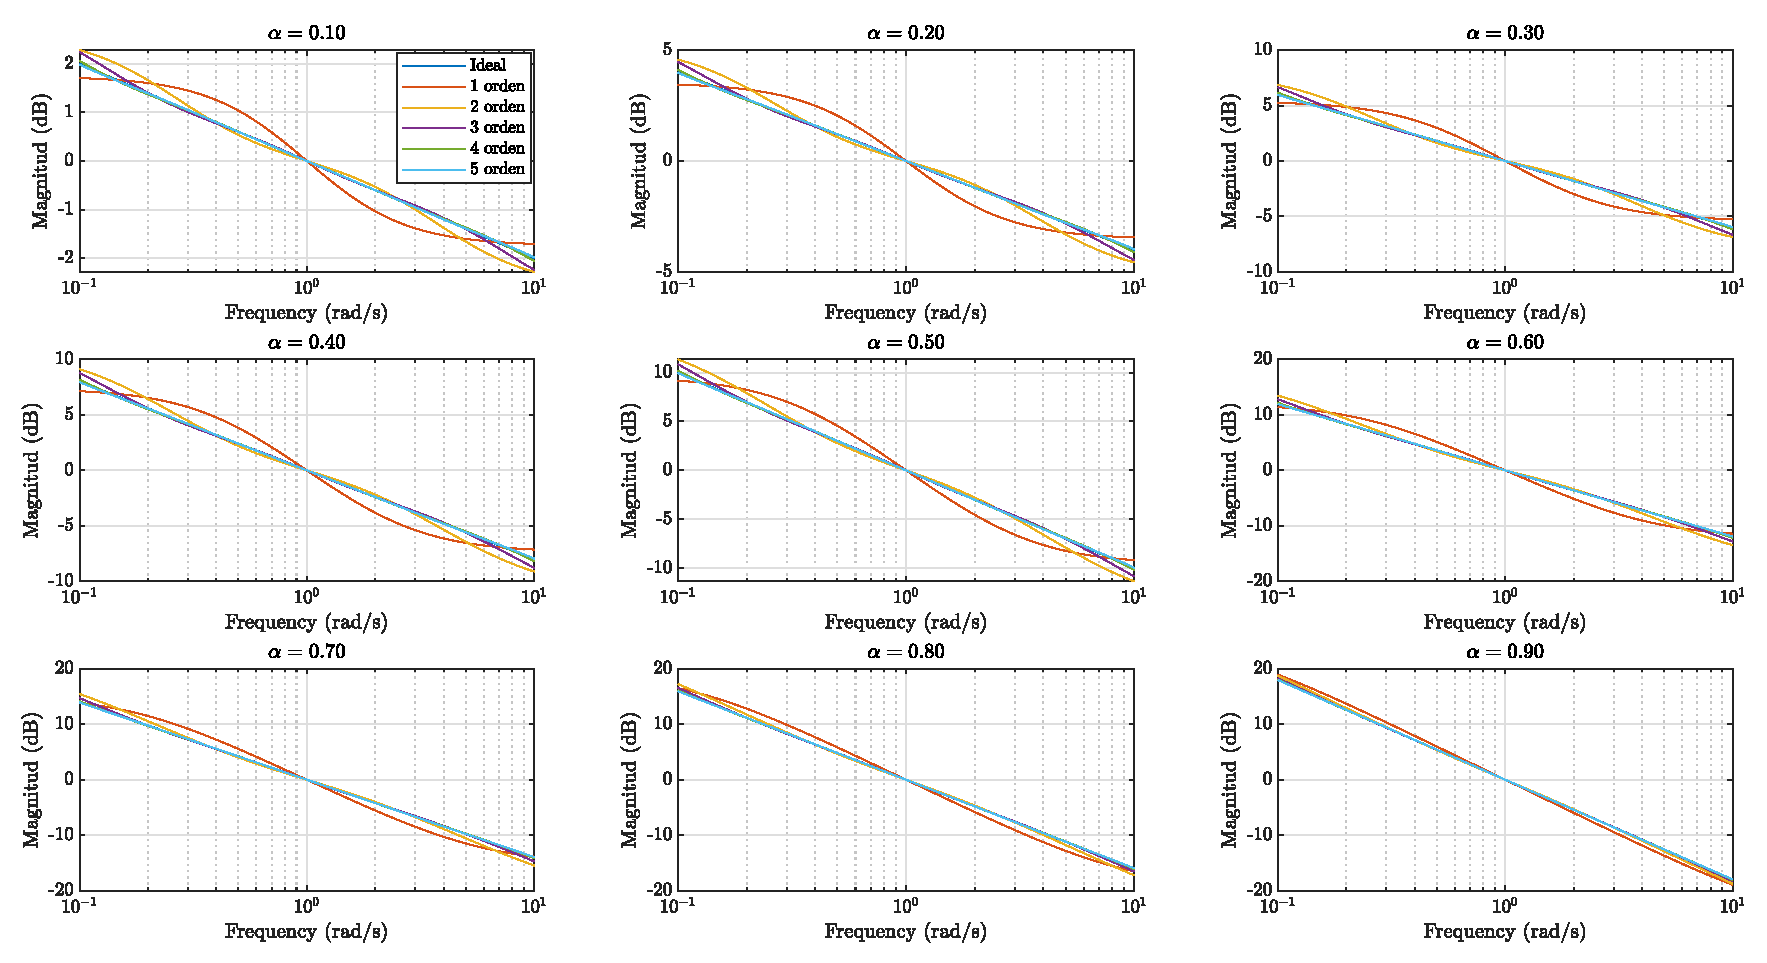
\includegraphics[width=0.93\textheight,angle=90]{F2_bode_magnitud_c.eps}
\end{figure}

\begin{figure}[hbtp]
	\caption{Diagramas de fase de aproximaciones de integrador fraccionario general.}
	\centering
	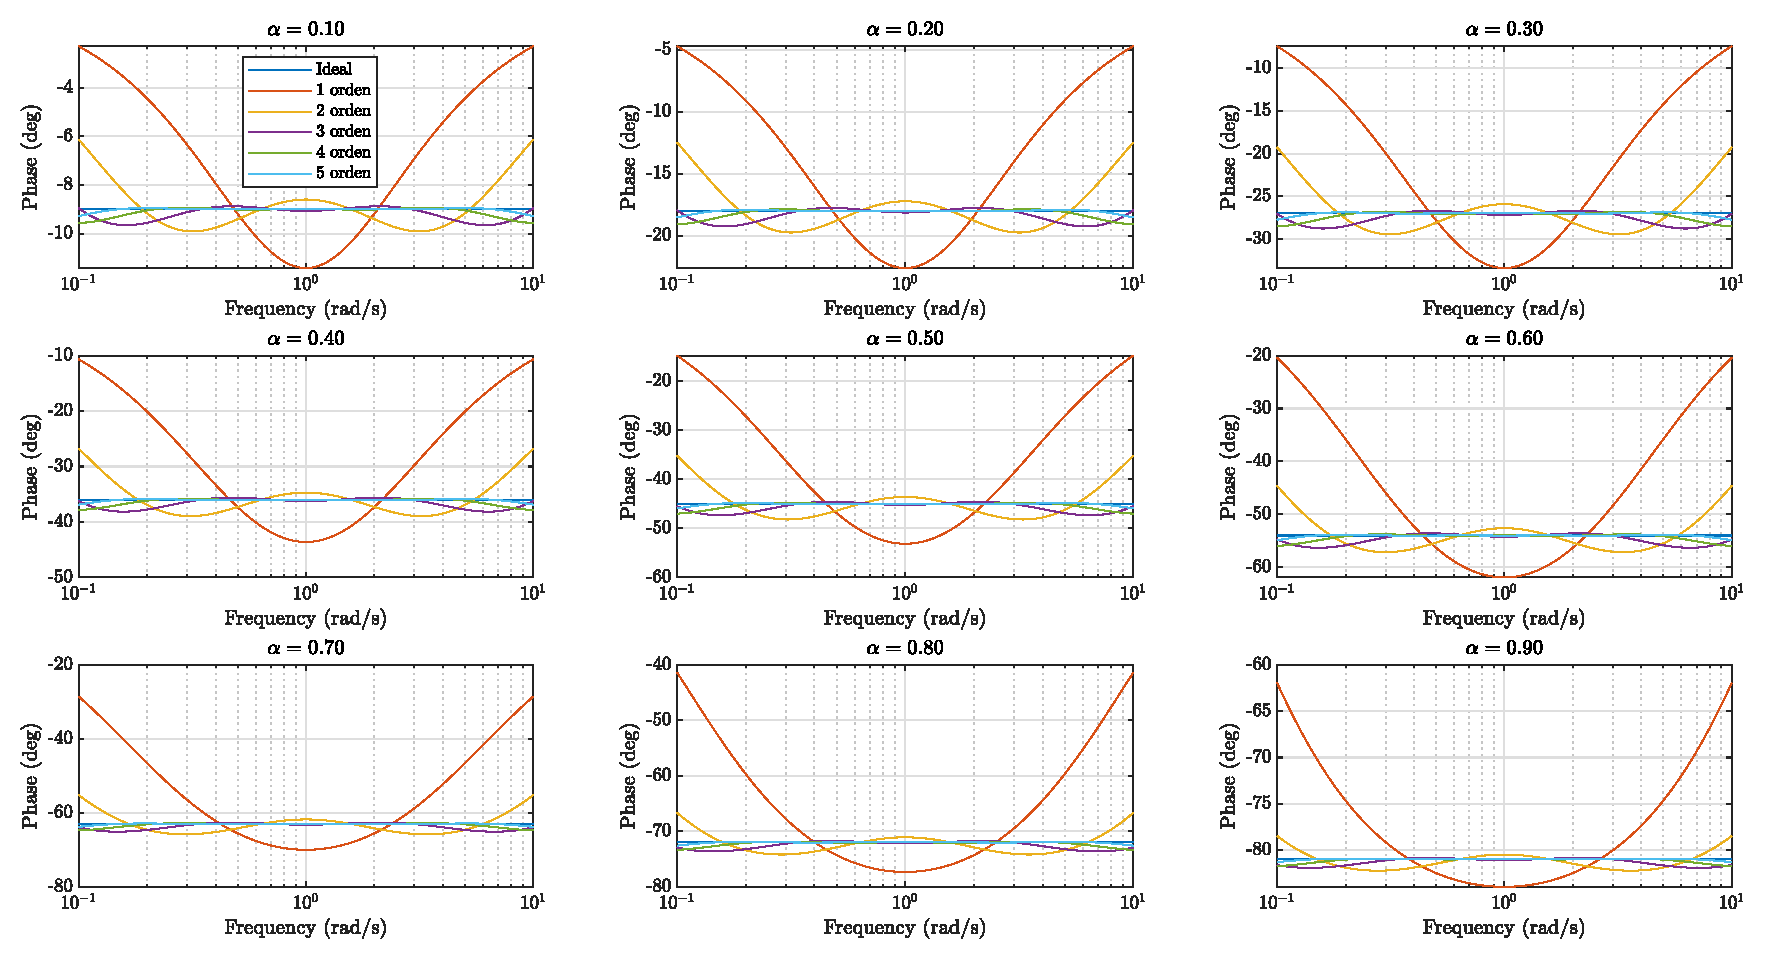
\includegraphics[width=0.93\textheight,angle=90]{F3_bode_fase_c.eps}
\end{figure}

\begin{figure}[hbtp]
	\caption{Diagramas de error de magnitud de aproximaciones de integrador fraccionario general.}
	\centering
	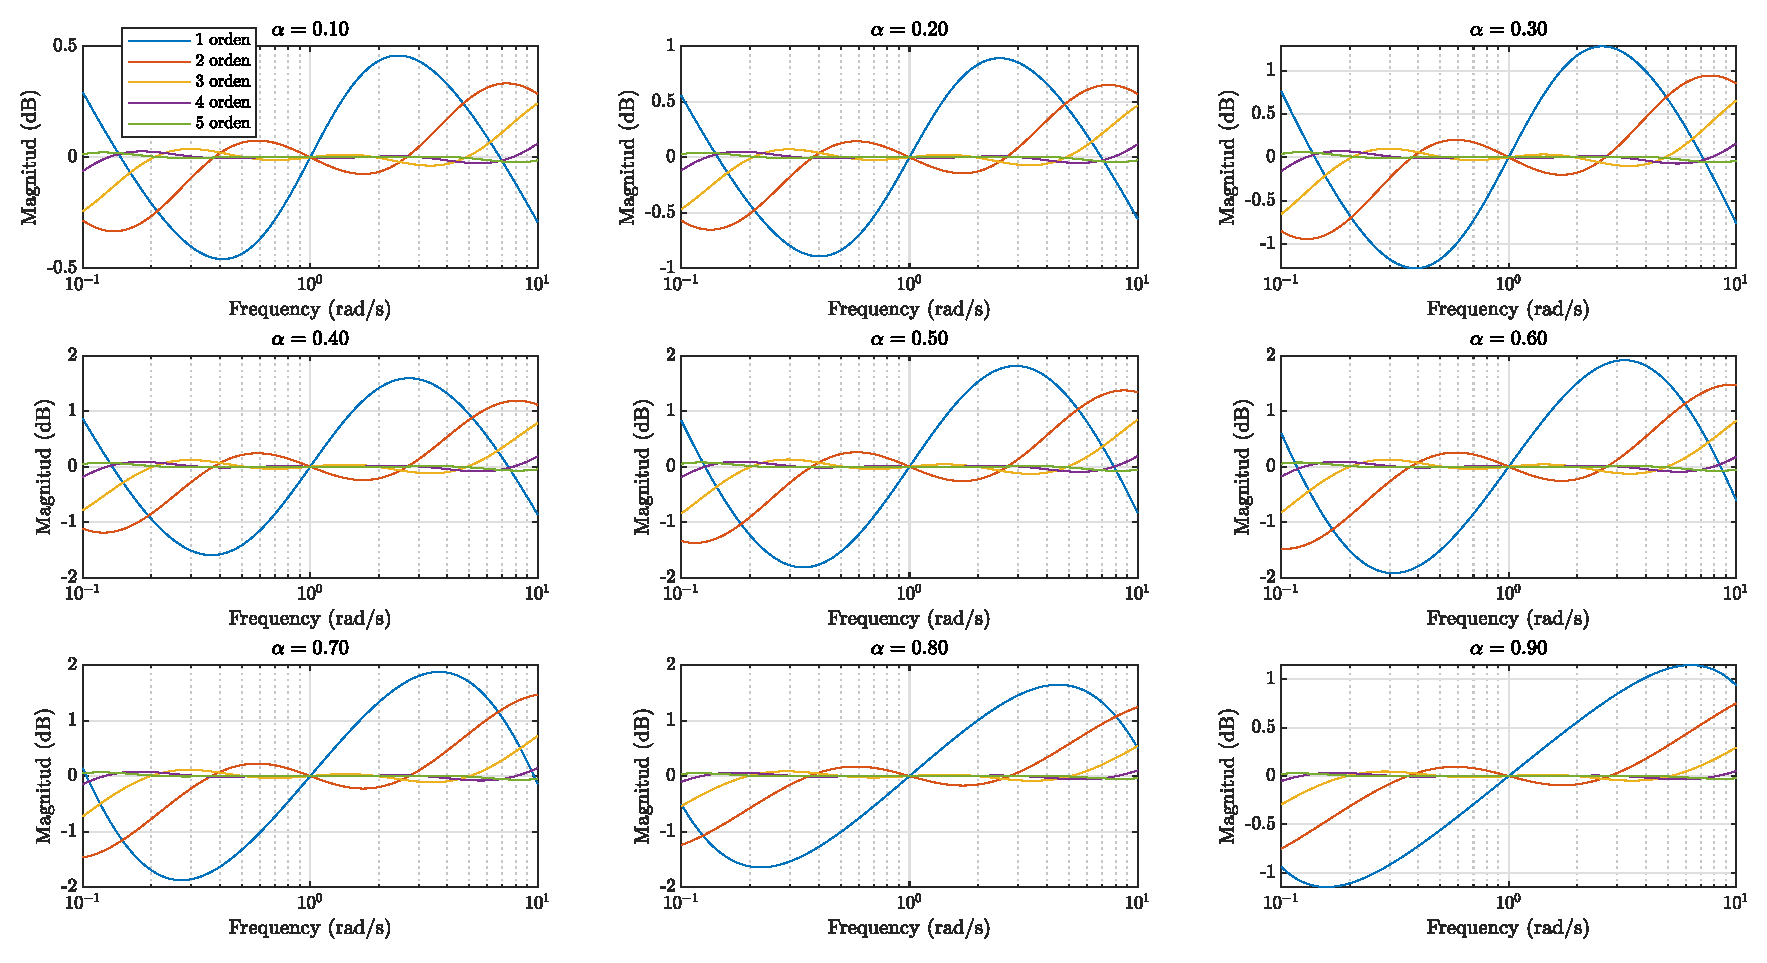
\includegraphics[width=0.93\textheight,angle=90]{F4_bode_error_mag_c.eps}
\end{figure}

\begin{figure}[hbtp]
	\caption{Diagramas de error de fase de aproximaciones de integrador fraccionario general.}
	\centering
	\includegraphics[width=0.93\textheight,angle=90]{F5_bode_error_fase_c.eps}
\end{figure}

%-------------------------------------------------------------------------------
%                            Graficas normalizadas                             %
%-------------------------------------------------------------------------------
\begin{figure}[hbtp]
	\caption{Diagramas de magnitud normalizada de aproximaciones de integrador fraccionario general.}
	\centering
	\includegraphics[width=0.93\textheight,angle=90]{F6_bode_magnitud_norm_c.eps}
\end{figure}

\begin{figure}[hbtp]
	\caption{Diagramas de fase normalizada de aproximaciones de integrador fraccionario general.}
	\centering
	\includegraphics[width=0.93\textheight,angle=90]{F7_bode_fase_norm_c.eps}
\end{figure}

\begin{figure}[hbtp]
	\caption{Diagramas de error de magnitud normalizada de aproximaciones de integrador fraccionario general.}
	\centering
	\includegraphics[width=0.93\textheight,angle=90]{F8_bode_error_mag_norm_c.eps}
\end{figure}

\begin{figure}[hbtp]
	\caption{Diagramas de error de fase normalizada de aproximaciones de integrador fraccionario general.}
	\centering
	\includegraphics[width=0.93\textheight,angle=90]{F9_bode_error_fase_norm_c.eps}
\end{figure}
	\chapter{Esquemático de QuadApex v2.0}

\begin{figure}[hbtp]
	\caption{Diagrama esquemático de QuadApex v2.0}
	\centering
	\includegraphics[width=16cm,angle=90]{Esquematico.eps}
	\label{fig:esquematico_fpaa}
\end{figure}

\backmatter

\bibliographystyle{ieeetr}
\bibliography{bibliografia}
\end{document}